\documentclass[10.5pt,a4paper]{article}
\usepackage[margin=18mm,top=16mm,bottom=18mm]{geometry}
\usepackage{amsmath,amssymb}
\usepackage{graphicx}
\usepackage{booktabs}
\usepackage{tabularx}
\usepackage{array}
\usepackage{enumitem}
\usepackage{natbib}
\usepackage[hidelinks]{hyperref}
\usepackage{microtype}
\usepackage[T1]{fontenc}
\usepackage[utf8]{inputenc}
\usepackage{lmodern}
\usepackage{xcolor}
\usepackage{titlesec}
\usepackage{tcolorbox}
\usepackage{caption}

\captionsetup{font=footnotesize,labelfont=bf,skip=3pt}

% Compact section styling
\titleformat{\section}[hang]{\normalfont\large\bfseries}{\thesection.\ }{0pt}{}
\titlespacing*{\section}{0pt}{6pt}{2pt}
\titleformat{\subsection}[hang]{\normalfont\normalsize\bfseries}{\thesubsection\ }{0pt}{}
\titlespacing*{\subsection}{0pt}{4pt}{2pt}
\titleformat{\subsubsection}[hang]{\normalfont\small\bfseries}{\thesubsubsection\ }{0pt}{}
\titlespacing*{\subsubsection}{0pt}{3pt}{1pt}

\graphicspath{{figures/}}
\setlength{\parindent}{0pt}
\setlength{\parskip}{0.28em}
\setlength{\emergencystretch}{2em}

% Custom table column types
\newcolumntype{L}[1]{>{\raggedright\arraybackslash}p{#1}}
\newcolumntype{C}[1]{>{\centering\arraybackslash}p{#1}}
\newcolumntype{R}[1]{>{\raggedleft\arraybackslash}p{#1}}
\newcolumntype{Y}{>{\raggedright\arraybackslash}X}

% Keep each figure's interpretation physically attached to the visual.
\newcommand{\figureconclusion}[1]{%
  \begin{tcolorbox}[
    colback=blue!2,
    colframe=blue!45!black,
    boxrule=0.35pt,
    arc=1pt,
    left=4pt,right=4pt,top=2pt,bottom=2pt,
    before skip=3pt,after skip=0pt]
    \footnotesize\textbf{Scientific conclusion.} #1
  \end{tcolorbox}%
}

\begin{document}

% Compact Title Block
\begin{center}
  {\Large\textbf{Application of Built-in Adaptive Remeshing and Mesh Refinement Features in Abaqus to Fracture Simulations Using Phase-field User Elements}}\\[0.3em]
  {\large\textbf{Comprehensive Mode-I Convergence \& UEL Energy Audit Supervisor Report -- 08 October 2026}}\\[0.2em]
  {\normalsize\textbf{Pruthviraja Reddy Vandavagali} (Matr. Nr. 68865) \quad $\cdot$ \quad Master Thesis in Computational Materials Science}\\[0.15em]
  {\footnotesize 1st Examiner: Prof. Dipl.-Ing. Bj\"orn Kiefer, Ph.D. \quad 2nd Examiner: Dr.-Ing. Stephan Roth \quad $\cdot$ \quad Chair of Applied Mechanics (IMFD), TU Bergakademie Freiberg}
\end{center}
\vspace{-0.4em}
\hrule height 0.6pt
\vspace{0.4em}

\section{Executive Summary and Governance Framework}
\label{sec:executive_summary}

\begin{tcolorbox}[colback=blue!5!white,colframe=blue!60!black,title=\textbf{Governing Supervisor Directive \& Active Phase},top=2pt,bottom=2pt,left=4pt,right=4pt]
\small
\emph{``We need to have understood everything related to the first model before we increase complexity.''}
\begin{center}
  \textbf{\texttt{MODE1\_GATE6B\_ENERGY\_CONVERGENCE\_AND\_STEP2\_QUALIFICATION\_ACTIVE}}
\end{center}
\end{tcolorbox}

Following the supervisor decisions of 17 September 2026, this report provides the comprehensive Mode-I convergence and energetic audit package for the 08 October 2026 supervisory review. The primary objective is to complete the physical, numerical, and energetic qualification of the Mode-I phase-field benchmark before advancing to state transfer, visualization integration, or multi-crack geometries.

\subsection{Status of governing milestone gates}
\begin{enumerate}[label=\textbf{\arabic*.},leftmargin=6mm,itemsep=2pt]
  \item \textbf{Gate 6A -- Mechanical Implementation \& Defect Closure:} \textbf{\texttt{RESOLVED\_AND\_CLOSED}}. The early 71,320-element initial stiffness defect was proven to arise from an Abaqus keyword preprocessing line limit ($\le 16$ nodes per line in \texttt{*NSET} without \texttt{GENERATE}), silently omitting 134 of 150 boundary nodes. Wrapping the data lines restored all constraints and achieved reference-consistent structural stiffness recovery (within $0.09\%$, $K_0 = 137.820804\,\mathrm{kN/mm}$ in full fracture Job \texttt{1404933}, $\Delta K_0 = -0.09\%$, $\Delta F_{\max} = -1.64\%$).
  \item \textbf{Gate 5 -- Native Remeshing Reproduction (71,320 vs $\approx 13{,}941$):} \textbf{\nolinkurl{SUPERVISOR_ACCEPTED_REPRODUCTION_LIMITATION_CLOSED}}. The supervisor accepted that publication details do not expose enough information to reproduce every reported element count exactly. Parametric sensitivity trends are preserved and strictly disambiguated between offline preliminary sizing ($1.0\% \to 71{,}320$; $2.0\% \to 17{,}687$; $3.0\% \to 8{,}120$; $5.0\% \to 4{,}356$) and the audited production batch meshes ($1.0\% \to 71{,}320$; $2.0\% \to 15{,}396$; $3.0\% \to 7{,}633$; $5.0\% \to 4{,}194$ finite elements).
  \item \textbf{Gate 6B -- Mode-I Energetic and Multifaceted Convergence:} \textbf{\texttt{ACTIVE -- HIGHEST PRIORITY}}. Decoupled evaluation across structural stiffness $K_0$, peak force $F_{\max}$, peak displacement $u_{\mathrm{peak}}$, trapezoidal boundary work $W_{\mathrm{trap}}$, UEL energy terms ($E_{\mathrm{elas}}, E_{\mathrm{frac}}$), crack-path symmetry, temporal discretization ($T_1$--$T_3$), spatial discretization ($S_1$--$S_4$), and length scale ($l_0$).
  \item \textbf{Global Energy Identity:} \textbf{\texttt{GLOBAL\_ENERGY\_IDENTITY --- NOT\_YET\_CLOSED}}. The staggered solution scheme evaluates history $\mathcal{H}_n$ at step $n$ and damage $d_{n+1}$ at step $n+1$, disproving the existence of a joint discrete scalar potential ($\partial^2 \Pi / \partial \mathbf{u} \partial d \ne \partial^2 \Pi / \partial d \partial \mathbf{u}$). Standard uninstrumented ODB files do not persist within-increment Newton paths.
  \item \textbf{Active Scope Holds:} Mode-II, Gate~6C (State Transfer), Gate~7 (Visualization integration), and multi-rank MPI remain on \textbf{strict hold} pending supervisor acceptance of Gate~6B closure.
\end{enumerate}

\subsection{Key scientific findings presented in this package}
\begin{itemize}[leftmargin=5mm,itemsep=2pt]
  \item \textbf{Energy Source Mechanical Parity:} Formally qualified as \textbf{\texttt{ENERGY\_SOURCE\_MECHANICAL\_PARITY --- QUALIFIED (COMMON QUAD FORMULATION)}}. Global mechanical force trajectories were identical ($|\Delta F| = 0.0\,\mathrm{kN}$) against uninstrumented baselines across both elastic (30 incs, Jobs 1406904 vs 1406905) and post-peak softening regimes ($u = 0.035\,\mathrm{mm}$, 129 incs, Jobs 1406906 vs 1406907). Old-run $d/\mathcal{H}$ state-field parity was not observable in ODBs and triangle parity was not established.
  \item \textbf{Single-IP Deduplication Rule:} Companion visualizer UMAT elements replicate scalar whole-element energies into all 4 Gauss integration points. Summing across all IPs creates an artificial $4\times$ overcounting error. Enforcing extraction at Integration Point 1 (\texttt{IP1}) recovers the once-per-underlying-finite-element global energy sum under the 2D implicit-unit-thickness convention.
  \item \textbf{Structural Stiffness Invariance:} Initial stiffness $K_0$ is exceptionally stable across spatial meshes ($S_1$--$S_4$: $137.95$ to $137.84\,\mathrm{kN/mm}$, spread $<0.09\%$), native adaptive meshes ($A_1$--$A_4$: spread $<0.09\%$), and time steps ($<0.001\%$), confirming kinematic, geometric, and elastic consistency.
  \item \textbf{Peak Force Mesh Sensitivity:} Peak reaction force drops monotonically with spatial mesh refinement from $0.7578\,\mathrm{kN}$ ($S_1$, $h/l_0 = 0.400$) to $0.7312\,\mathrm{kN}$ ($S_4$, $h/l_0 = 0.167$), extending to $0.7255\,\mathrm{kN}$ on the historical fine mesh ($h = 1.0\,\mu\mathrm{m}$, $-4.26\%$ total variation), classified as \textbf{\texttt{MESH-SENSITIVE}}.
  \item \textbf{Crack-Path Symmetry and Profile Convergence:} The damage-weighted crack-centroid trajectory deviates from the symmetry plane $y = 0.500\,\mathrm{mm}$ by $\le 3.10\,\mu\mathrm{m}$ across all fixed and adaptive meshes, confirming pure Mode-I symmetry within discrete element bounds. Ligament damage profiles agree closely during the pre-peak regime across all meshes, while diverging near peak load where localized damage develops.
  \item \textbf{Completed 3-Point Length-Scale Study ($l_0$):} Evaluated across $l_0 \in \{7.5, 11.25, 15.0\}\,\mu\mathrm{m}$ on fixed $S_3$ mesh (Jobs \texttt{1406017.mmaster02}, \texttt{1406895.mmaster02}, \texttt{1406896.mmaster02}). $K_0$ is stable ($137.86 \to 137.68\,\mathrm{kN/mm}$, $0.13\%$ spread), while $F_{\max}$ ($0.7322 \to 0.6895\,\mathrm{kN}$) and $u_{\mathrm{peak}}$ ($5.633 \to 5.579\,\mu\mathrm{m}$) are length-scale sensitive. Terminal energy comparison across unequal endpoints is classified as \textbf{\texttt{NOT\_YET\_QUALIFIED\_UNEQUAL\_ENDPOINTS}}.
\end{itemize}

\clearpage

\section{Mode-I Benchmark Definition and Canonical S1 Reference Baseline}
\label{sec:benchmark_and_reference}

\subsection{Benchmark Boundary Value Problem}
The Mode-I benchmark is defined on a two-dimensional square domain $\Omega = [0, 1.0\,\mathrm{mm}] \times [0, 1.0\,\mathrm{mm}]$ containing an initial sharp horizontal edge crack of length $a_0 = 0.50\,\mathrm{mm}$ along the symmetry plane $y = 0.50\,\mathrm{mm}$ (Fig.~\ref{fig:mode1_geometry_pack}). The crack is discretized as a zero-gap seam with duplicate coincident nodal lines, preserving exact geometric compliance.

\begin{figure}[htbp]
  \centering
  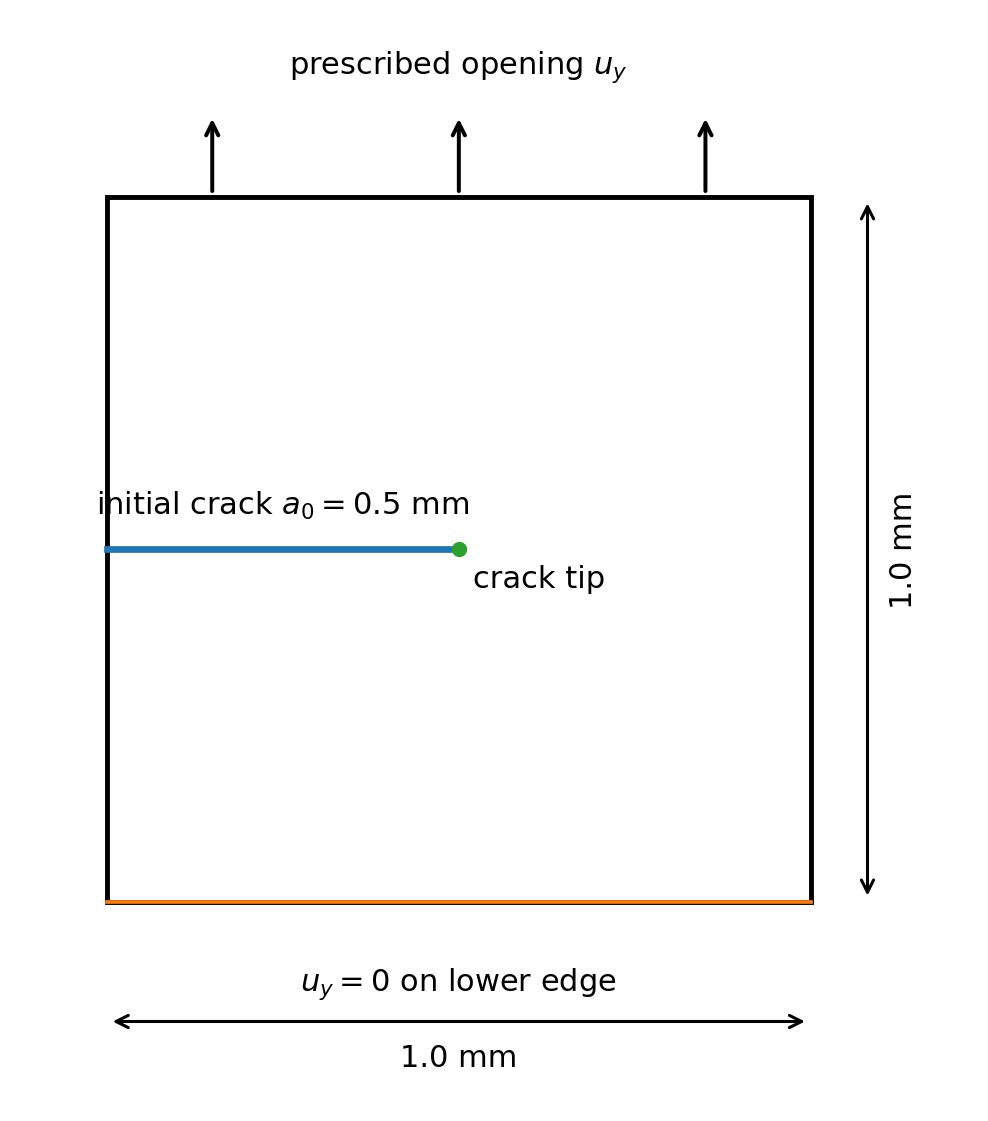
\includegraphics[width=0.48\textwidth]{fig_mode1_geometry.png}
  \caption{Mode-I benchmark boundary value problem: $1.0\,\mathrm{mm} \times 1.0\,\mathrm{mm}$ square domain with a sharp edge crack of length $a_0 = 0.5\,\mathrm{mm}$ along $y = 0.5\,\mathrm{mm}$. Boundary conditions enforce roller support ($u_y = 0$) on the bottom edge with a pinned point ($u_x = 0$) to eliminate rigid-body motion, and uniform tensile displacement $u_y = u$ on the top edge.}
  \label{fig:mode1_geometry_pack}
  \figureconclusion{This figure fixes the governed physical boundary-value problem. All later fixed and adaptive simulations use the same geometry, supports, and loading, so their differences can be attributed to discretization, time stepping, or adaptivity rather than to a changed model definition.}
\end{figure}

The material and phase-field constitutive parameters follow \citet{pandey2025}:
\begin{itemize}[noitemsep,topsep=1pt]
  \item Young's modulus: $E = 210.0\,\mathrm{GPa} = 210.0\,\mathrm{kN/mm^2}$;
  \item Poisson's ratio: $\nu = 0.30$;
  \item Critical fracture energy release rate: $G_c = 2.7 \times 10^{-3}\,\mathrm{kN/mm}$ ($2.7\,\mathrm{N/mm}$);
  \item Phase-field regularization length scale: $l_0 = 0.0075\,\mathrm{mm} = 7.5\,\mu\mathrm{m}$;
  \item Residual stiffness parameter: $k_{\mathrm{res}} = 1.0 \times 10^{-7}$.
\end{itemize}

\subsection{Boundary-Condition Verification and Seam Compliance}
A vital early physical distinction is that global initial structural stiffness $K_0 = \Delta F / \Delta u$ is a structural property, distinct from the material Young's modulus $E$. During initial model verification, representing the crack as a finite-width notch was found to introduce substantial artificial compliance ($K_0 \approx 75.47\,\mathrm{kN/mm}$). The geometry was therefore corrected to the required zero-gap sharp seam before the governed convergence and adaptive-remeshing studies were performed. All subsequent results use the corrected sharp-seam geometry.

\subsection{Canonical S1 Baseline Provenance}
\begingroup\small
The governed canonical baseline for the Mode-I benchmark is Job \texttt{1406015.mmaster02} ($S_1$, $15{,}192$ underlying finite elements, $15{,}522$ total \texttt{*NODE} entries ($15{,}521$ mesh nodes + RP 999999)), generated from the canonical input deck (\texttt{SHA256: bc000e0c5791150a\allowbreak711cb7af447a0bb3\allowbreak4d1b9d9af5c6ce9d\allowbreak096c98749e8edf61}). Extracted from the audited source file \nolinkurl{S1_h0030_15k_MECHANICAL_FU_AUDITED.csv} (\texttt{SHA256: E3100B7429E14B8B\allowbreak CEAB9952DDF8B041\allowbreak 9CA9F71DF058F591\allowbreak 6668922185AA25E2}) over the initial $N = 400$ active increments ($u \le 1.0\,\mu\mathrm{m}$), unconstrained ordinary least squares yields:
\begin{equation}
  \boxed{K_0 = 137.945520\,\mathrm{kN/mm}}, \quad b = 4.472368 \times 10^{-5}\,\mathrm{kN}, \quad R^2 = 0.99999960.
\end{equation}
The peak reaction force is $F_{\max} = 0.757778\,\mathrm{kN}$ at displacement $u(F_{\max}) = 0.005857\,\mathrm{mm}$, matching digitized literature values from \citet{pandey2025} ($F_{\max} \approx 0.758\,\mathrm{kN}, u \approx 0.005860\,\mathrm{mm}$). Reconstructed Job \texttt{1398090.mmaster02} is preserved as historical baseline evidence. This canonical response provides the quantitative anchor against which all spatial, temporal, and adaptive remeshing results are judged.
\par\endgroup

\clearpage

\section{Pandey--Kumar Adaptive Refinement and MISESERI Mechanism}
\label{sec:adaptive_method_miseseri}

\subsection{Two-Job Adaptive Refinement Procedure}
\citet{pandey2025} employ an automated two-job pre-refinement procedure:
\begin{center}
\setlength{\fboxsep}{4pt}
\fbox{Coarse Job-1 (Layered UEL/UMAT)}
$\rightarrow$ \fbox{Pre-Analysis Stage 1 (500 incs)}
$\rightarrow$ \fbox{\texttt{MISESERI} Field Extraction}
$\rightarrow$ \fbox{\texttt{RemeshingRule}}
$\rightarrow$ \fbox{\texttt{adaptiveRemesh}}
$\rightarrow$ \fbox{Job-2 Multi-Layer Generation}
$\rightarrow$ \fbox{Nonlinear Fracture Solve}.
\end{center}

\begin{figure}[htbp]
  \centering
  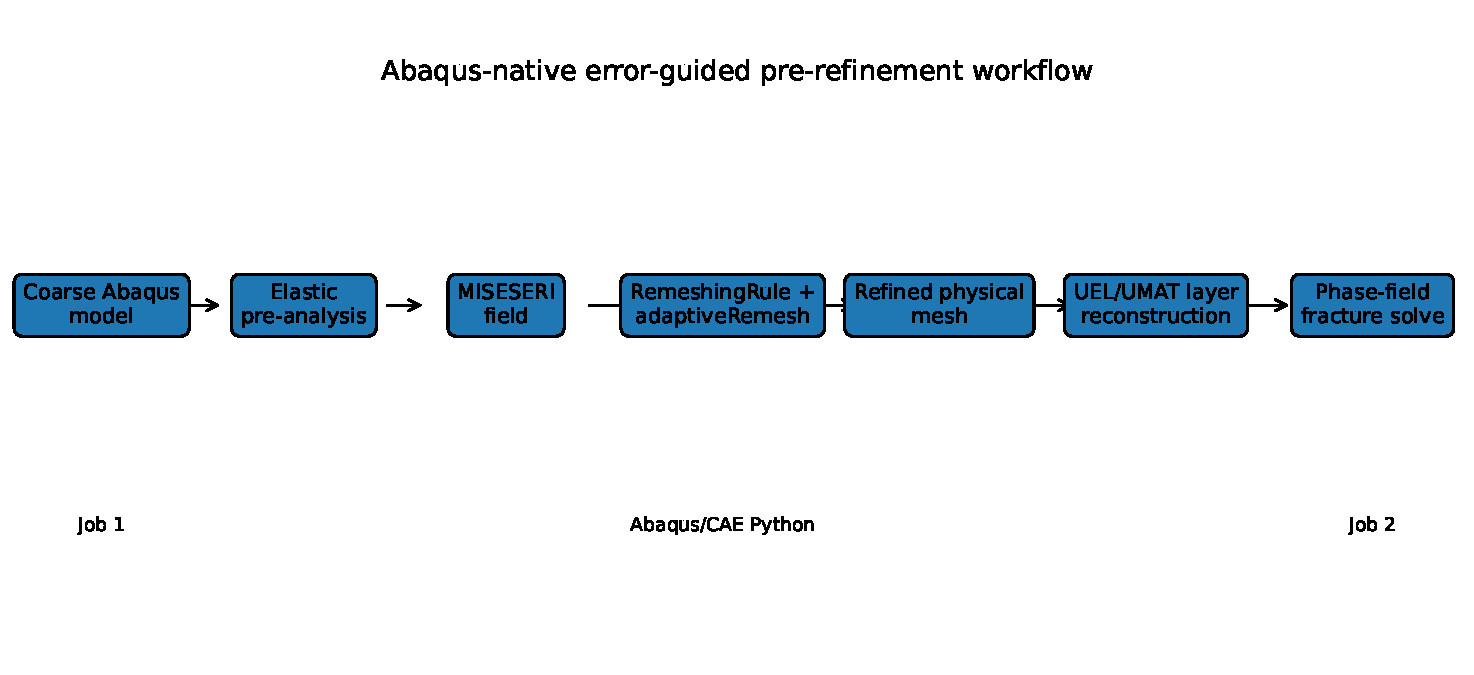
\includegraphics[width=0.85\textwidth]{fig_refinement_workflow.pdf}
  \caption{Pandey--Kumar two-job adaptive pre-refinement workflow: a coarse pre-analysis on the layered UEL/UMAT model evaluates stress recovery error on the co-located continuum layer, which drives native \texttt{adaptiveRemesh} before reconstructing the multi-layer UEL/UMAT phase-field model.}
  \label{fig:refinement_workflow_pack}
  \figureconclusion{The method is an error-driven \emph{pre-refinement} workflow, not remeshing during crack propagation: the mesh is generated before the nonlinear phase-field fracture solve begins.}
\end{figure}

The published Mode-I description outlines a 500-increment first loading stage followed by a 1000-increment second stage. However, the exact \texttt{stepName} and frame selection semantics used within the native \texttt{RemeshingRule} are not explicitly disclosed in the publication.

\subsection{Physical Understanding and Provenance of MISESERI}
\texttt{MISESERI} is the Abaqus stress discretization error indicator associated with the recovered von Mises stress field in linear continuum elasticity \citep{abaqus2023}. It is based on stress-recovery error estimation on the linear-elastic continuum stress field; it is \textbf{not} phase-field error, \textbf{not} damage error, and \textbf{not} fracture energy imbalance.

\begin{figure}[htbp]
  \centering
  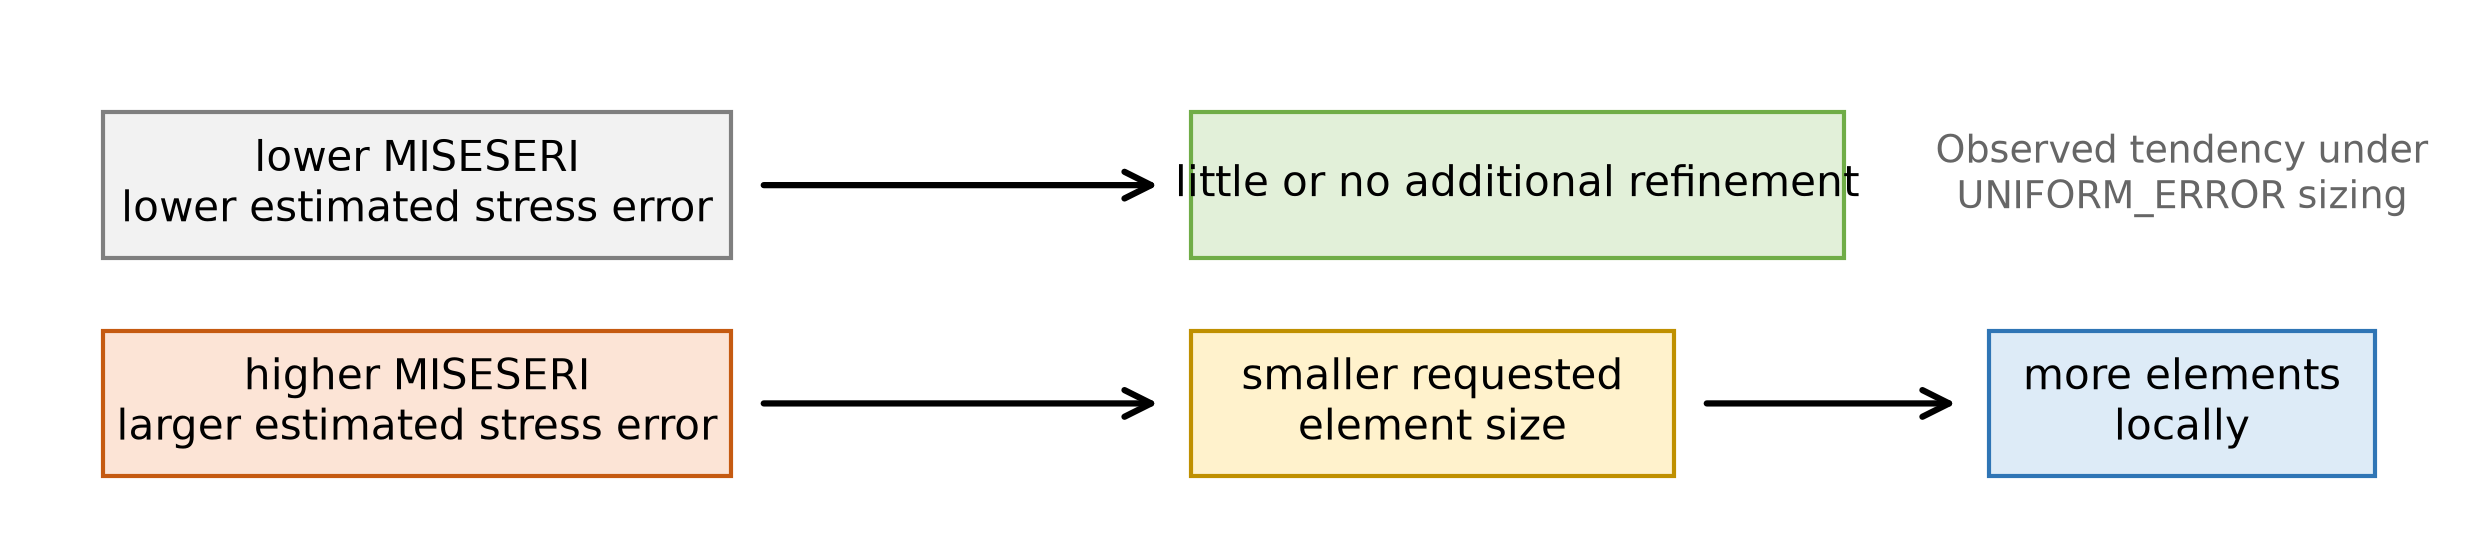
\includegraphics[width=0.88\textwidth]{fig_miseseri_concept.png}
  \caption{Directional relationship of \texttt{MISESERI} under uniform-error sizing: elevated stress error near singularities dictates local refinement without representing a direct algebraic formula to element size.}
  \label{fig:miseseri_concept_pack}
  \figureconclusion{Higher recovered-stress discretization error promotes stronger local refinement, but \texttt{errorTarget} is a target tolerance rather than a direct \texttt{MISESERI} threshold or an explicit formula for element size.}
\end{figure}

The sizing parameter \texttt{errorTarget=1.0} in Listing~1 of \citet{pandey2025} denotes a $1.0\%$ target error tolerance under \texttt{UNIFORM\_ERROR} sizing. It does \textbf{not} mean $\mathtt{MISESERI} = 1.0$ or that $1\%$ of elements are refined. Similarly, \texttt{errorTarget=2.0} specifies a $2.0\%$ target tolerance, not $\mathtt{MISESERI} = 2.0$.

\subsection{Canonical Mode-I Pre-Analysis and Spatial Association}
The canonical Mode-I pre-analysis contains $2{,}906$ finite elements ($2{,}818$ CPE4 + $88$ CPE3), $2{,}988$ nodes, and exactly $2{,}906$ scalar \texttt{WHOLE\_ELEMENT} \texttt{MISESERI} indicator values (Fig.~\ref{fig:miseseri_error_map_pack}).

\begin{figure}[htbp]
  \centering
  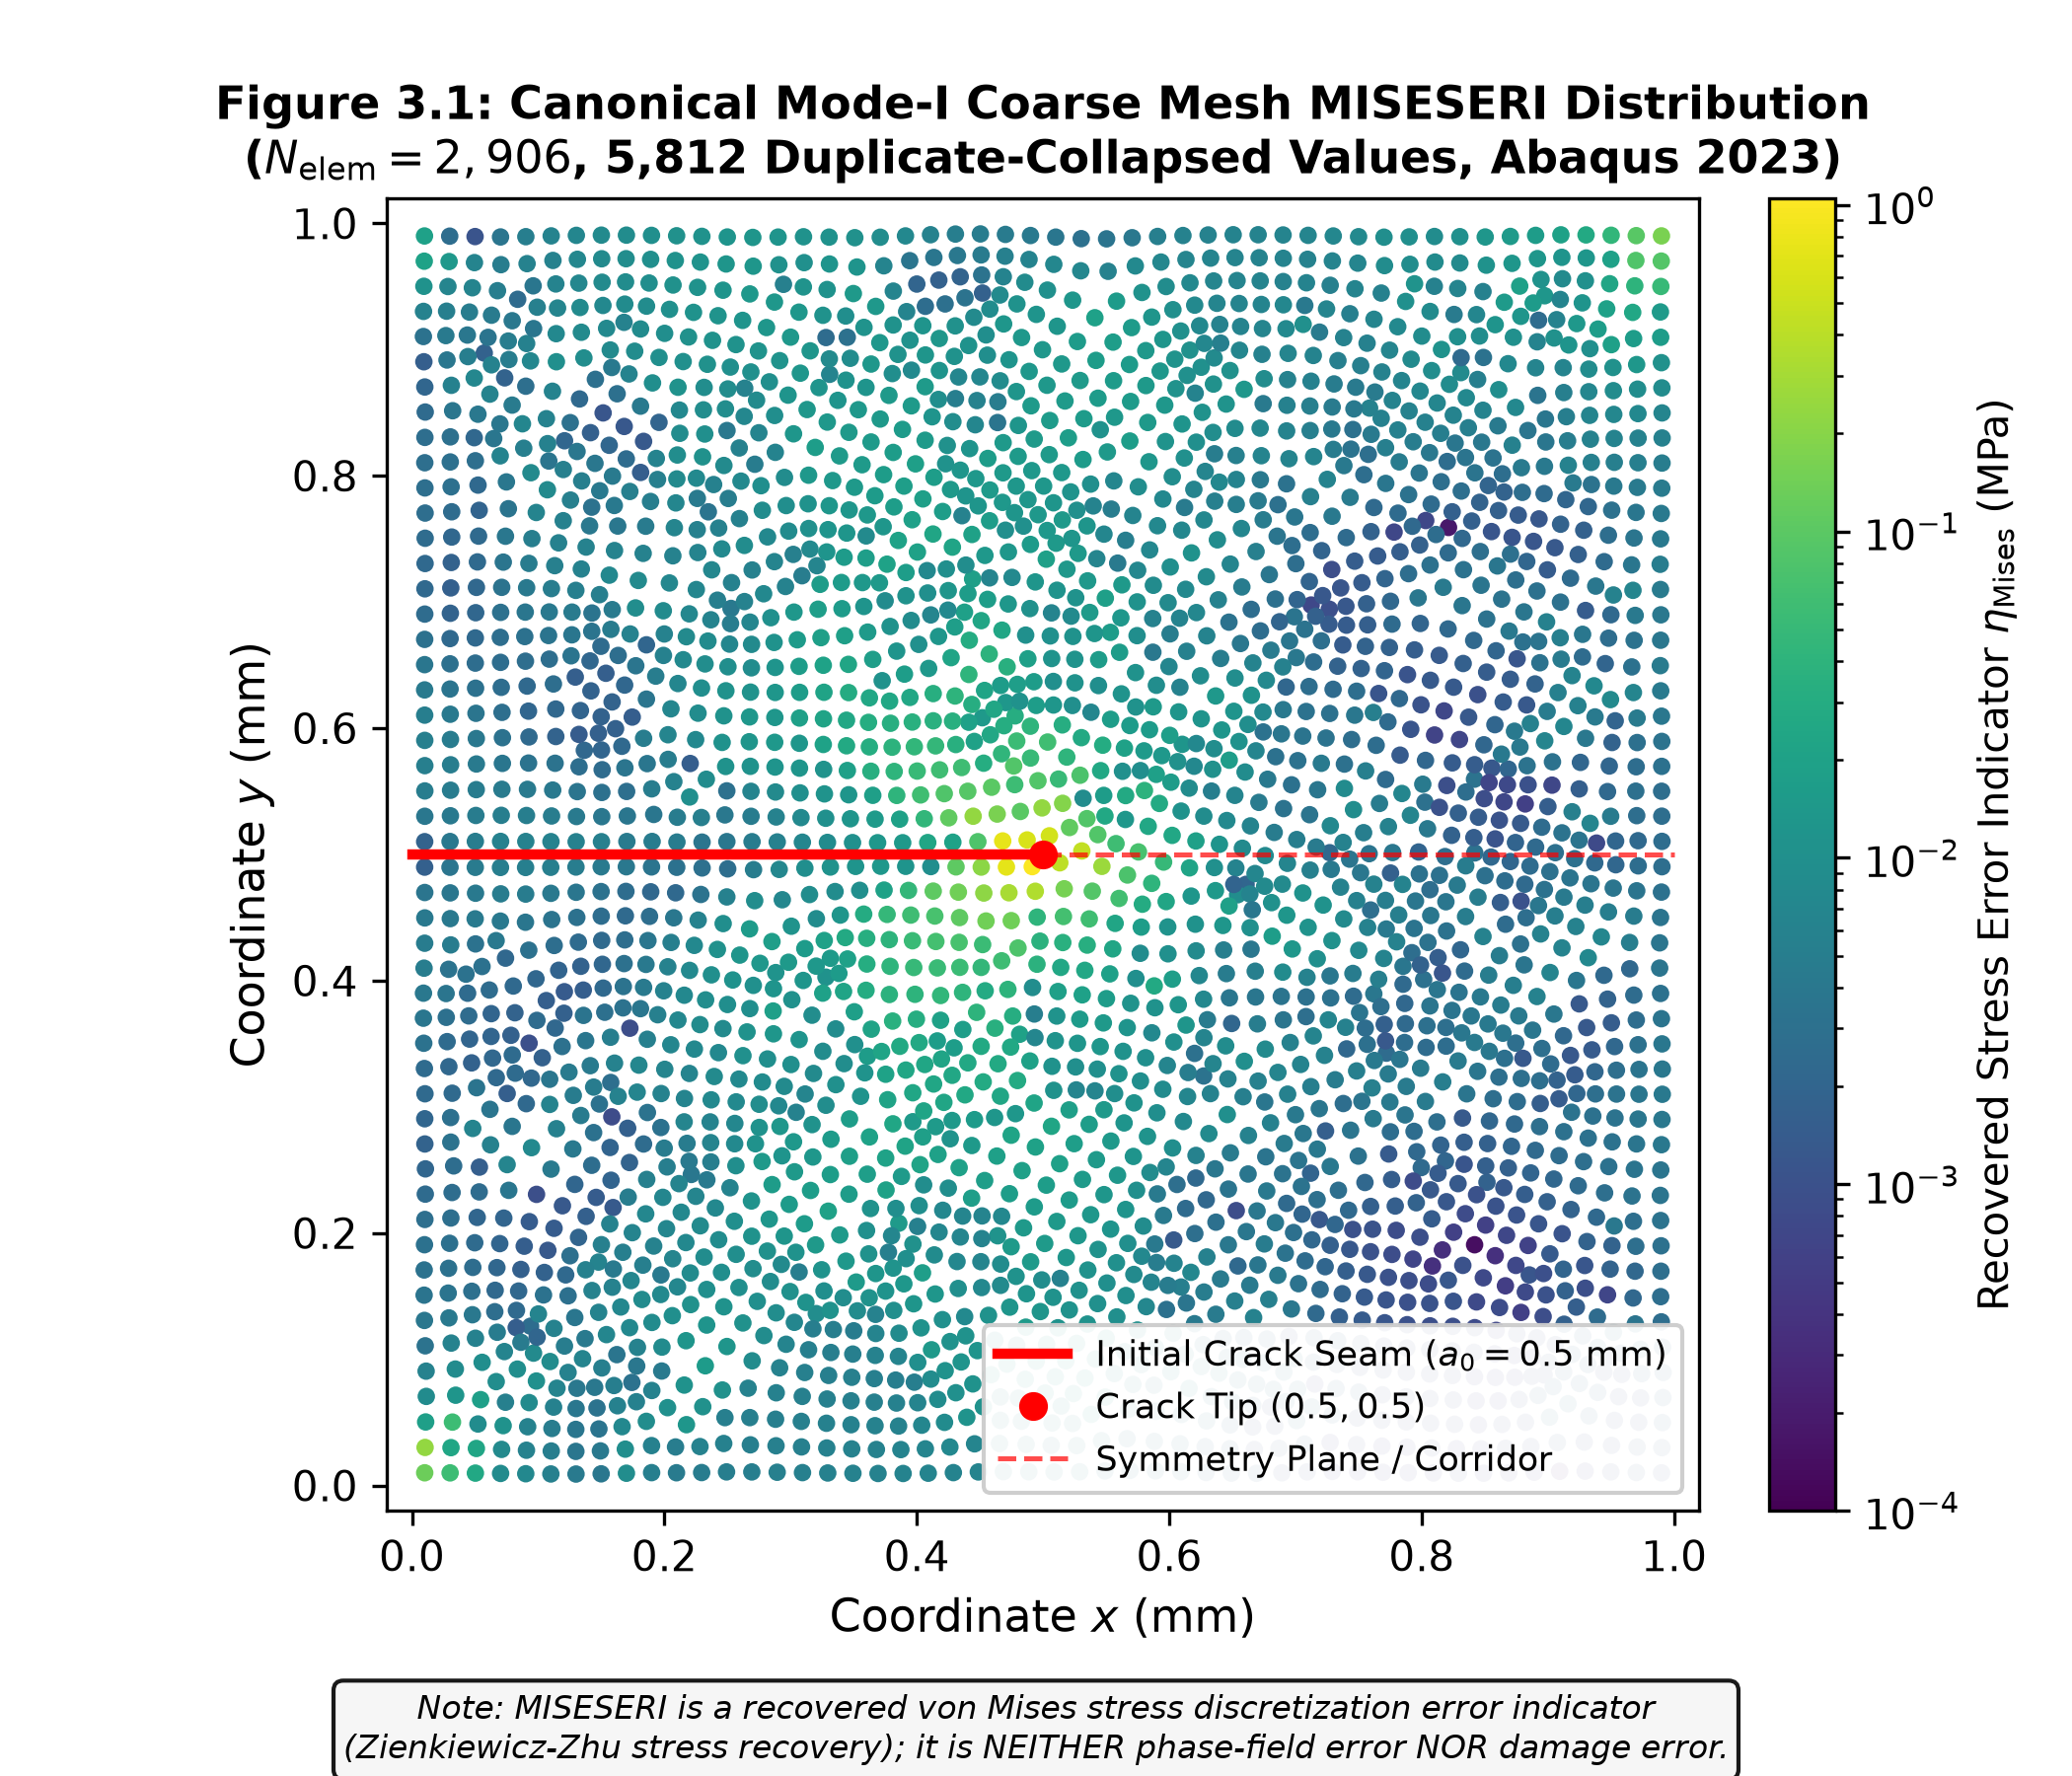
\includegraphics[width=0.88\textwidth]{figure_3_1_canonical_mode1_miseseri_error_map.png}
  \caption{Canonical Mode-I \texttt{MISESERI} error indicator field evaluated on the 2,906-element coarse mesh, showing error concentration at the initial crack tip.}
  \label{fig:miseseri_error_map_pack}
  \figureconclusion{The coarse elastic mesh is most under-resolved around the initial crack tip, where the stress gradient is highest. \texttt{MISESERI} is a stress discretization-error indicator, not a phase-field or damage-error measure.}
\end{figure}

Applying \texttt{errorTarget=1.0\%} with \texttt{coarseningFactor=NOT\_ALLOWED} generates the 71,320-element mesh (Fig.~\ref{fig:coarse_vs_adapted_pack}). As shown in Fig.~\ref{fig:miseseri_association_pack}, adapted element sizes correlate closely with the coarse indicator field.

\begin{figure}[htbp]
  \centering
  \begin{minipage}{0.48\textwidth}
    \centering
    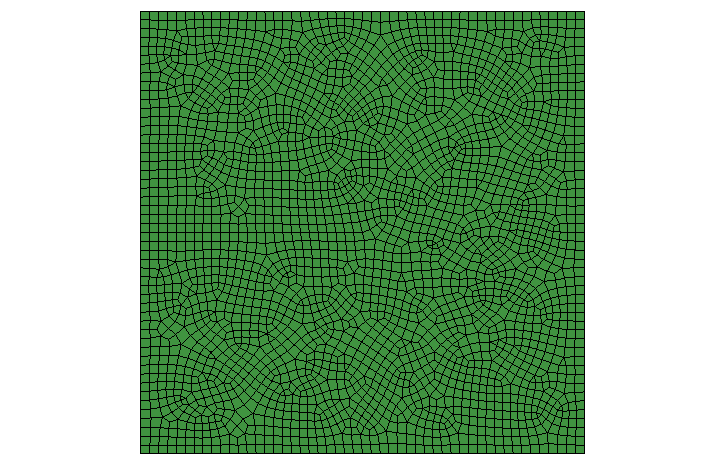
\includegraphics[width=\textwidth]{fig03a_coarse_mesh_cae.png}
    \caption*{(a) Coarse pre-analysis mesh ($2{,}906$ elements)}
  \end{minipage}\hfill
  \begin{minipage}{0.48\textwidth}
    \centering
    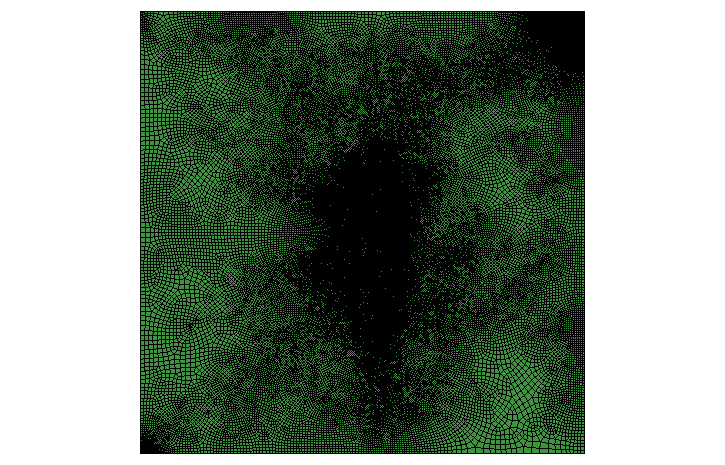
\includegraphics[width=\textwidth]{fig13_adaptive_71320_mesh_cae.png}
    \caption*{(b) Adapted mesh ($71{,}320$ elements)}
  \end{minipage}
  \caption{Visual comparison of (a) initial coarse mesh ($2{,}906$ elements) and (b) native adapted mesh ($71{,}320$ elements).}
  \label{fig:coarse_vs_adapted_pack}
  \figureconclusion{Abaqus converts the nonuniform error field into the expected nonuniform mesh: element density is concentrated along the crack-tip corridor while regions farther away remain comparatively coarse.}
\end{figure}

\begin{figure}[htbp]
  \centering
  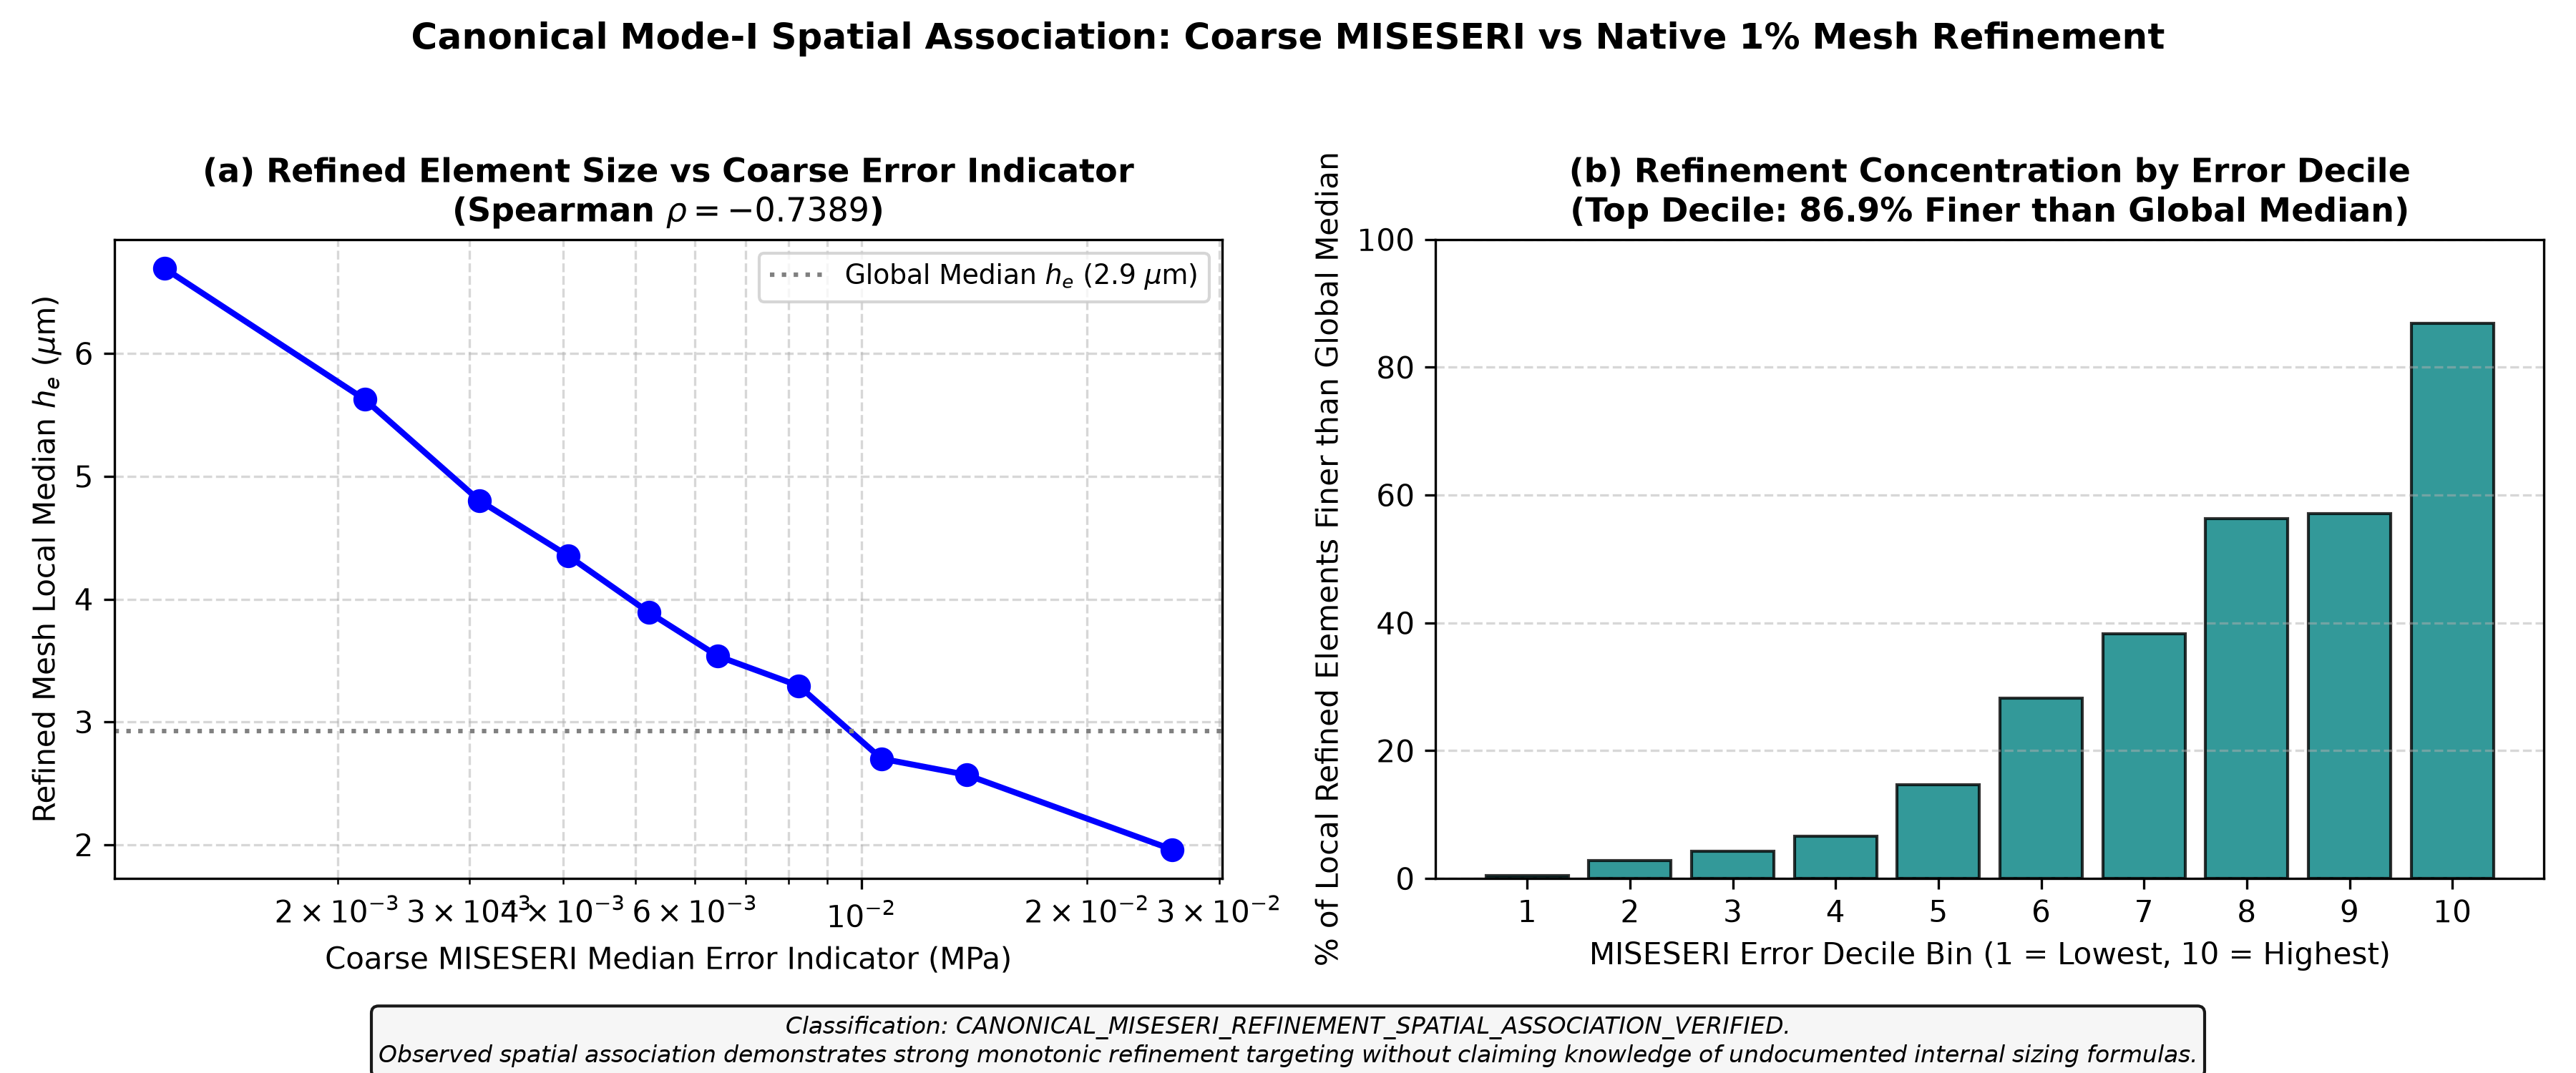
\includegraphics[width=0.82\textwidth]{fig_miseseri_spatial_association.png}
  \caption{Empirical spatial association between coarse \texttt{MISESERI} and adapted element size $h$ for the Mode-I benchmark.}
  \label{fig:miseseri_association_pack}
  \figureconclusion{Large coarse-mesh \texttt{MISESERI} values are spatially associated with small adapted elements. This verifies error-guided refinement without claiming an exact proprietary \texttt{MISESERI}$\rightarrow h$ mapping law.}
\end{figure}

\clearpage

\section{Resolution of the 71,320-Element Boundary Formatting Defect}
\label{sec:stiffness_anomaly_resolution}

\subsection{Defect Mechanism and Verified Resolution}
An early 71,320-element adaptive model (historical Job \texttt{1399632}) exhibited an artificial stiffness deficit caused by an Abaqus keyword input card limit: the bottom-edge node set \texttt{N\_BOTTOM} contained 150 node identifiers written on a single data line without \texttt{GENERATE}. Abaqus \texttt{pre} parsed only the first 16 node entries and silently omitted the remaining 134 nodes from the constraint set.

Wrapping the \texttt{N\_BOTTOM} data across valid data lines ($\le 16$ entries per line) fully constrained all 150 intended bottom nodes, restoring the structural stiffness to the reference range. The defect was independently verified and is formally classified as \textbf{\texttt{RESOLVED\_AND\_CLOSED}}; all subsequent adaptive results use the corrected boundary-condition definition.

The two authoritative verification runs confirm full mechanical recovery (Table~\ref{tab:nbottom_summary_pack} and Fig.~\ref{fig:mode1_fu_recovery_pack}):
\begin{itemize}[noitemsep,topsep=2pt]
  \item \textbf{Corrected Full Fracture (Job \texttt{1404933.mmaster02}):} Solved the complete fracture process, achieving $K_0 = 137.820804\,\mathrm{kN/mm}$ ($\Delta K_0 = -0.09\%$) and peak load $F_{\max} = 0.745325\,\mathrm{kN}$ ($\Delta F_{\max} = -1.64\%$).
  \item \textbf{Frozen Elastic Requalification (Job \texttt{1405044.mmaster02}):} Independent elastic verification achieving $K_0 = 138.021013\,\mathrm{kN/mm}$ ($\Delta K_0 = +0.05\%$) with zero node lift and zero warnings.
\end{itemize}

\begin{table}[htbp]
\centering
\caption{Mechanical response recovery after resolving the \texttt{N\_BOTTOM} keyword line limit.}
\label{tab:nbottom_summary_pack}
\small
\begin{tabularx}{\textwidth}{lrrrrY}
\toprule
Case Description & Job ID & Elements & $K_0$ [kN/mm] & $F_{\max}$ [kN] & Status / Governed Role \\
\midrule
Fixed Reference Anchor ($S_1$) & \texttt{1406015} & $15{,}192$ & $137.945520$ & $0.757778$ & Canonical reference anchor \\
Corrected Full Fracture ($A_1$) & \texttt{1404933} & $71{,}320$ & $137.820804$ & $0.745325$ & Production $1\%$ adaptive mesh \\
Frozen Elastic Requalification & \texttt{1405044} & $71{,}320$ & $138.021013$ & -- & Independent elastic verification \\
\bottomrule
\end{tabularx}
\end{table}

\begin{figure}[htbp]
  \centering
  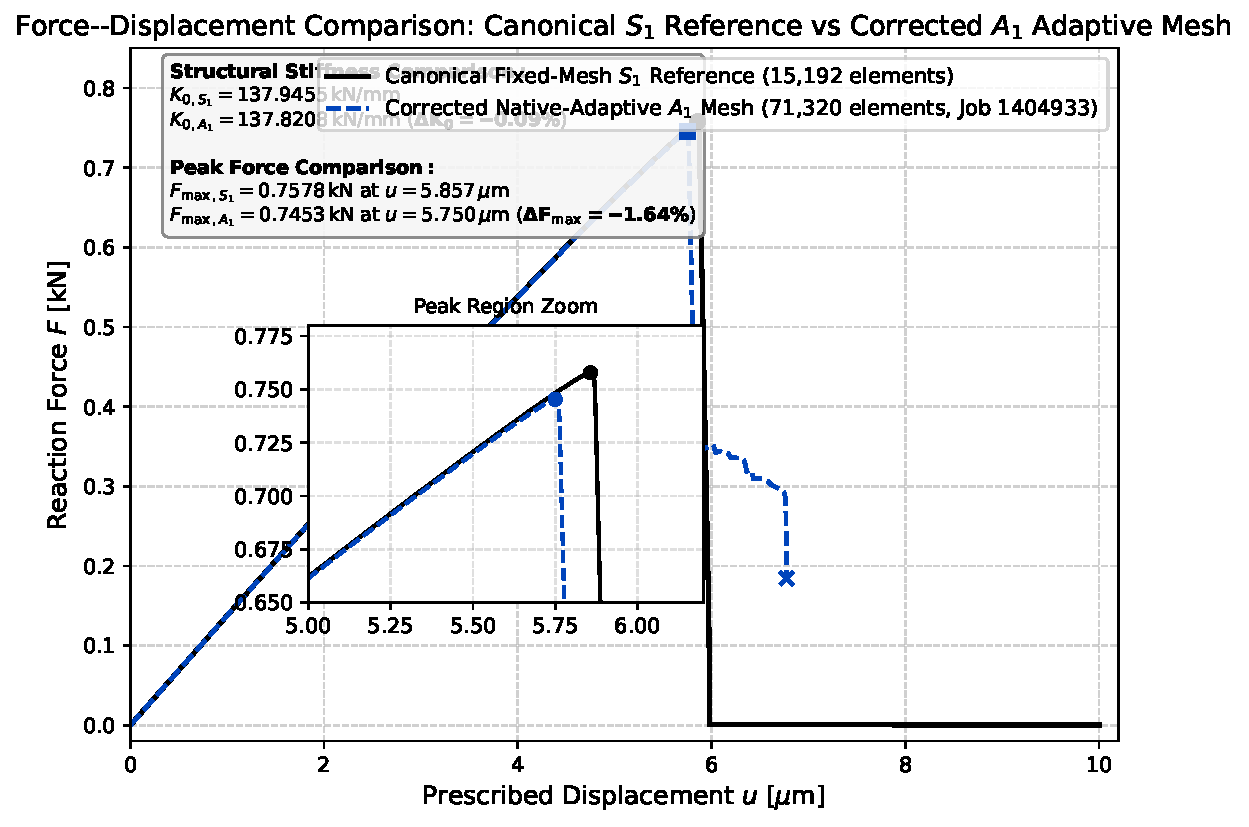
\includegraphics[width=0.82\textwidth]{fig_mode1_fu_recovery.pdf}
  \caption{Force--displacement comparison between the canonical fixed-mesh $S_1$ reference ($15{,}192$ finite elements) and the corrected native-adaptive $A_1$ model with \texttt{errorTarget = 1\%} ($71{,}320$ finite elements). The initial structural stiffness differs by only $0.09\%$, while the adaptive peak reaction force is approximately $1.64\%$ below the reference value.}
  \label{fig:mode1_fu_recovery_pack}
  \figureconclusion{Correcting \texttt{N\_BOTTOM} restores the adaptive model's elastic stiffness. The remaining peak-force difference is therefore a fracture/discretization effect, not evidence of an unresolved elastic boundary-condition defect.}
\end{figure}

\clearpage

\section{Discrepancy Audit: 71,320 vs 13,941 Elements and Governing Decision}
\label{sec:discrepancy_audit_71k_vs_14k}

\subsection{Publication Discrepancy and Comprehensive Investigation}
\citet{pandey2025} report an adapted Mode-I element count of $\approx 13{,}941$, while strictly applying the published Listing~1 settings to the full domain generates $71{,}320$ finite elements.

An exhaustive numerical and software investigation established:
\begin{enumerate}
  \item \textbf{Abaqus Release Invariance:} Abaqus 2019 GA, 2021.HF26, 2022 GA, and 2023.HF4 all generate $100.000\%$ bitwise identical $71{,}320$-element meshes with matching SHA-256 hashes.
  \item \textbf{Single-Factor Parameter Testing:} Testing load magnitude, output frequency, boundary conditions, and mesher controls ruled out trivial parameter differences.
  \item \textbf{Regional Breakdown:} The crack process corridor ($|y| \le 0.05\,\mathrm{mm}$) contains $9{,}061$ elements ($12.7\%$), while far-field and transition regions contain $62{,}259$ elements ($87.3\%$) because coarsening was disabled (\texttt{coarseningFactor=NOT\_ALLOWED}).
  \item \textbf{Pre-Analysis Loading and Step Lineage:} Evaluating native remeshing against the qualified two-step layered UEL/UMAT pre-analysis (Job \texttt{1409554.mmaster02}) deterministically yields $48{,}329$ finite elements ($48{,}093$ nodes) under $1.0\%$ error target ($100.000\%$ mesh identity across independent repeats). An interim provisional run (Job \texttt{1409546.mmaster02}) yielded $42{,}318$ elements.
\end{enumerate}

\subsection{Supervisor Decision and Definitive Closure}
During the meeting on 17 September 2026, the supervisor formally closed this investigation under the following governing ruling:
\begin{center}
  \textbf{\texttt{SUPERVISOR\_ACCEPTED\_REPRODUCTION\_LIMITATION\_CLOSED}}
\end{center}
The supervisor confirmed that:
\begin{itemize}
  \item The complete author code, internal scripts, and exact frame selection routines are unavailable;
  \item The publication does not disclose sufficient information to reproduce the specific $13{,}941$ element count;
  \item The reproducible $48{,}329$-element mesh is classified as \textbf{\texttt{PROJECT\_REPRODUCIBLE\_STEP1\_1PCT\_RESULT}}, not an authoritative literature match;
  \item The remaining difference between $48{,}329$ and $13{,}941$, along with the exact step/frame filtering semantics, is formally designated as \textbf{\texttt{UNRESOLVED\_PUBLICATION\_IMPLEMENTATION\_DETAIL}} and \textbf{\texttt{FRAME\_SELECTION\_SEMANTICS\_UNRESOLVED}};
  \item Exact $13{,}941$ reproduction is \textbf{not an active blocker};
  \item Reproduction of general error-guided adaptivity trends is fully sufficient;
  \item Additional effort aimed solely at discovering an unpublished detail is not justified;
  \item All tested sensitivity results shall be preserved in the thesis as documented evidence.
\end{itemize}

\subsection{Preserved Parametric Sensitivity Trends}
Table~\ref{tab:error_target_sensitivity_pack} summarizes the preserved sensitivity results across four target error tolerances, demonstrating monotonic mesh reduction as tolerance relaxes.

\begin{table}[htbp]
\centering
\caption{Parametric sensitivity of adapted finite element counts to the \texttt{errorTarget} tolerance.}
\label{tab:error_target_sensitivity_pack}
\begin{tabular}{lrrrl}
\toprule
Case & \texttt{errorTarget} & Coarse Baseline Count & Corrected Pre-Analysis Count & Classification \\
\midrule
$A_1$ & $1.0\%$ & $71{,}320$ & $48{,}329$ & Reproducible Step-1 1\% result \\
$A_2$ & $2.0\%$ & $17{,}687$ & $11{,}737$ & $2.0\%$ error tolerance \\
$A_3$ & $3.0\%$ & $8{,}120$ & $5{,}158$ & $3.0\%$ error tolerance \\
$A_4$ & $5.0\%$ & $4{,}356$ & $3{,}763$ & $5.0\%$ error tolerance \\
\bottomrule
\end{tabular}
\end{table}

\clearpage

\section{Multifaceted Mode-I Convergence Evaluation}
\label{sec:multifaceted_convergence}

In accordance with supervisor directives, mesh adequacy and numerical convergence are evaluated across multiple complementary physical and energetic quantities rather than peak reaction force alone.

\subsection{Spatial Mesh Resolution Series ($S_1$--$S_4$)}
Four uniform meshes spanning element edge lengths from $h = 3.0\,\mu\mathrm{m}$ ($S_1$, $15{,}192$ elements) down to $h = 1.25\,\mu\mathrm{m}$ ($S_4$, $51{,}408$ elements) evaluate spatial discretization characteristics ($h/l_0 \in [0.167, 0.400]$ at fixed $l_0 = 7.5\,\mu\mathrm{m}$), alongside a separate historical fine-mesh result ($h = 1.0\,\mu\mathrm{m}$, $69{,}384$ elements, Job \texttt{1406019.mmaster02}):
\begin{enumerate}
  \item \textbf{Initial Structural Stiffness $K_0$ is Stable:} Across the governed $S_1$--$S_4$ spatial series, $K_0$ varies from $137.945520$ to $137.841200\,\mathrm{kN/mm}$. An additional historical $h=1.0\,\mu\mathrm{m}$ mesh gives $137.823301\,\mathrm{kN/mm}$, confirming that the initial structural stiffness remains exceptionally stable over the broader tested resolution range ($< 0.09\%$ total variation, $R^2 > 0.999999$). Classified as \textbf{\texttt{CONVERGED / STABLE}}.
  \item \textbf{Peak Force $F_{\max}$ and Displacement $u_{\mathrm{peak}}$ are Mesh-Sensitive:} Across the full tested range, peak force decreases monotonically from $0.7578\,\mathrm{kN}$ ($S_1$) to $0.7255\,\mathrm{kN}$ (historical fine mesh), a total reduction of $4.26\%$ (Fig.~\ref{fig:spatial_fu_pack} and \ref{fig:spatial_metrics_pack}). The displacement at peak load shifts from $5.857$ to $5.575\,\mu\mathrm{m}$, corresponding to an approximately $4.81\%$ earlier peak with refinement. Classified as \textbf{\texttt{MESH-SENSITIVE}}.
\end{enumerate}

\begin{figure}[htbp]
  \centering
  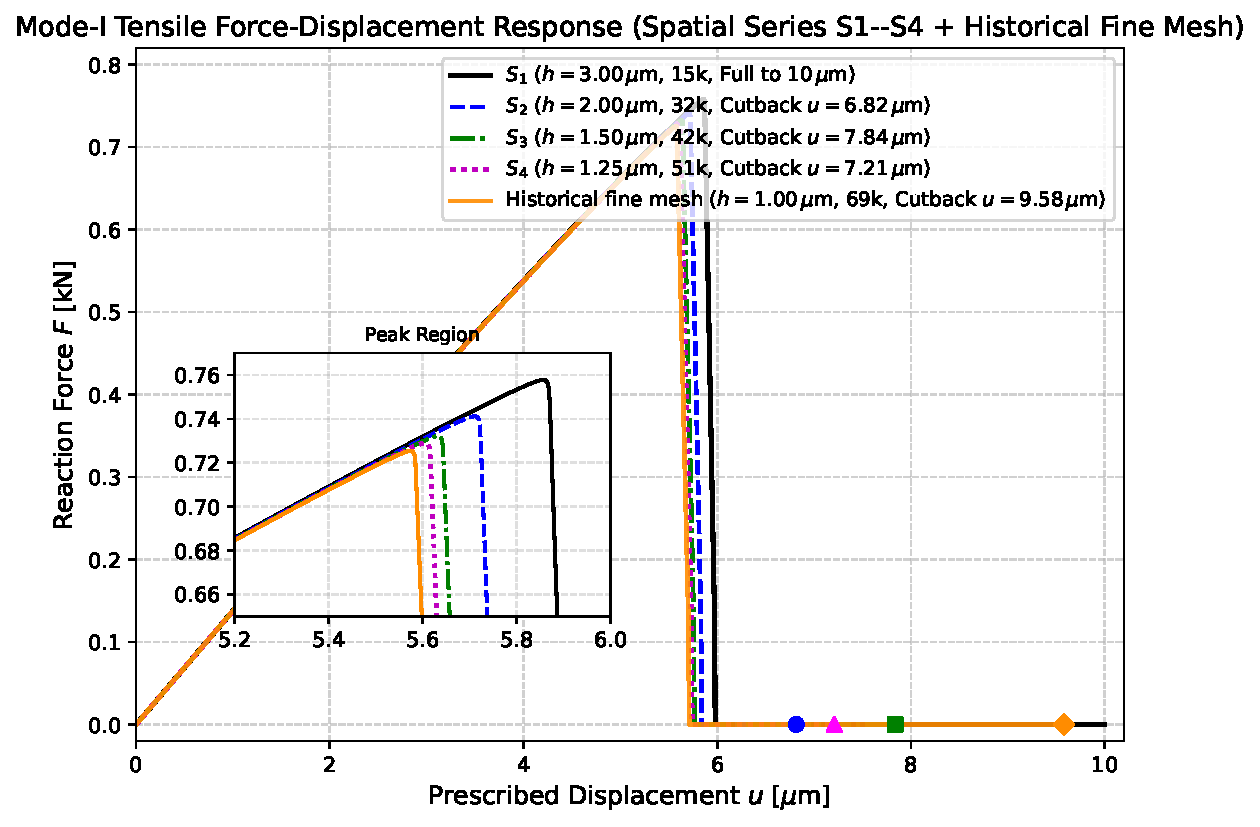
\includegraphics[width=0.82\textwidth]{fig_mode1_spatial_fu_convergence.pdf}
  \caption{Mode-I tensile force-displacement response across uniform mesh resolutions ($S_1$--$S_4$ plus historical fine mesh), showing identical elastic stiffness and systematic peak load mesh sensitivity.}
  \label{fig:spatial_fu_pack}
  \figureconclusion{The elastic slopes are effectively mesh-independent, but refinement systematically lowers $F_{\max}$ and shifts $u_{\mathrm{peak}}$ earlier. Elastic response is stable; fracture initiation remains spatially mesh-sensitive.}
\end{figure}

\begin{figure}[htbp]
  \centering
  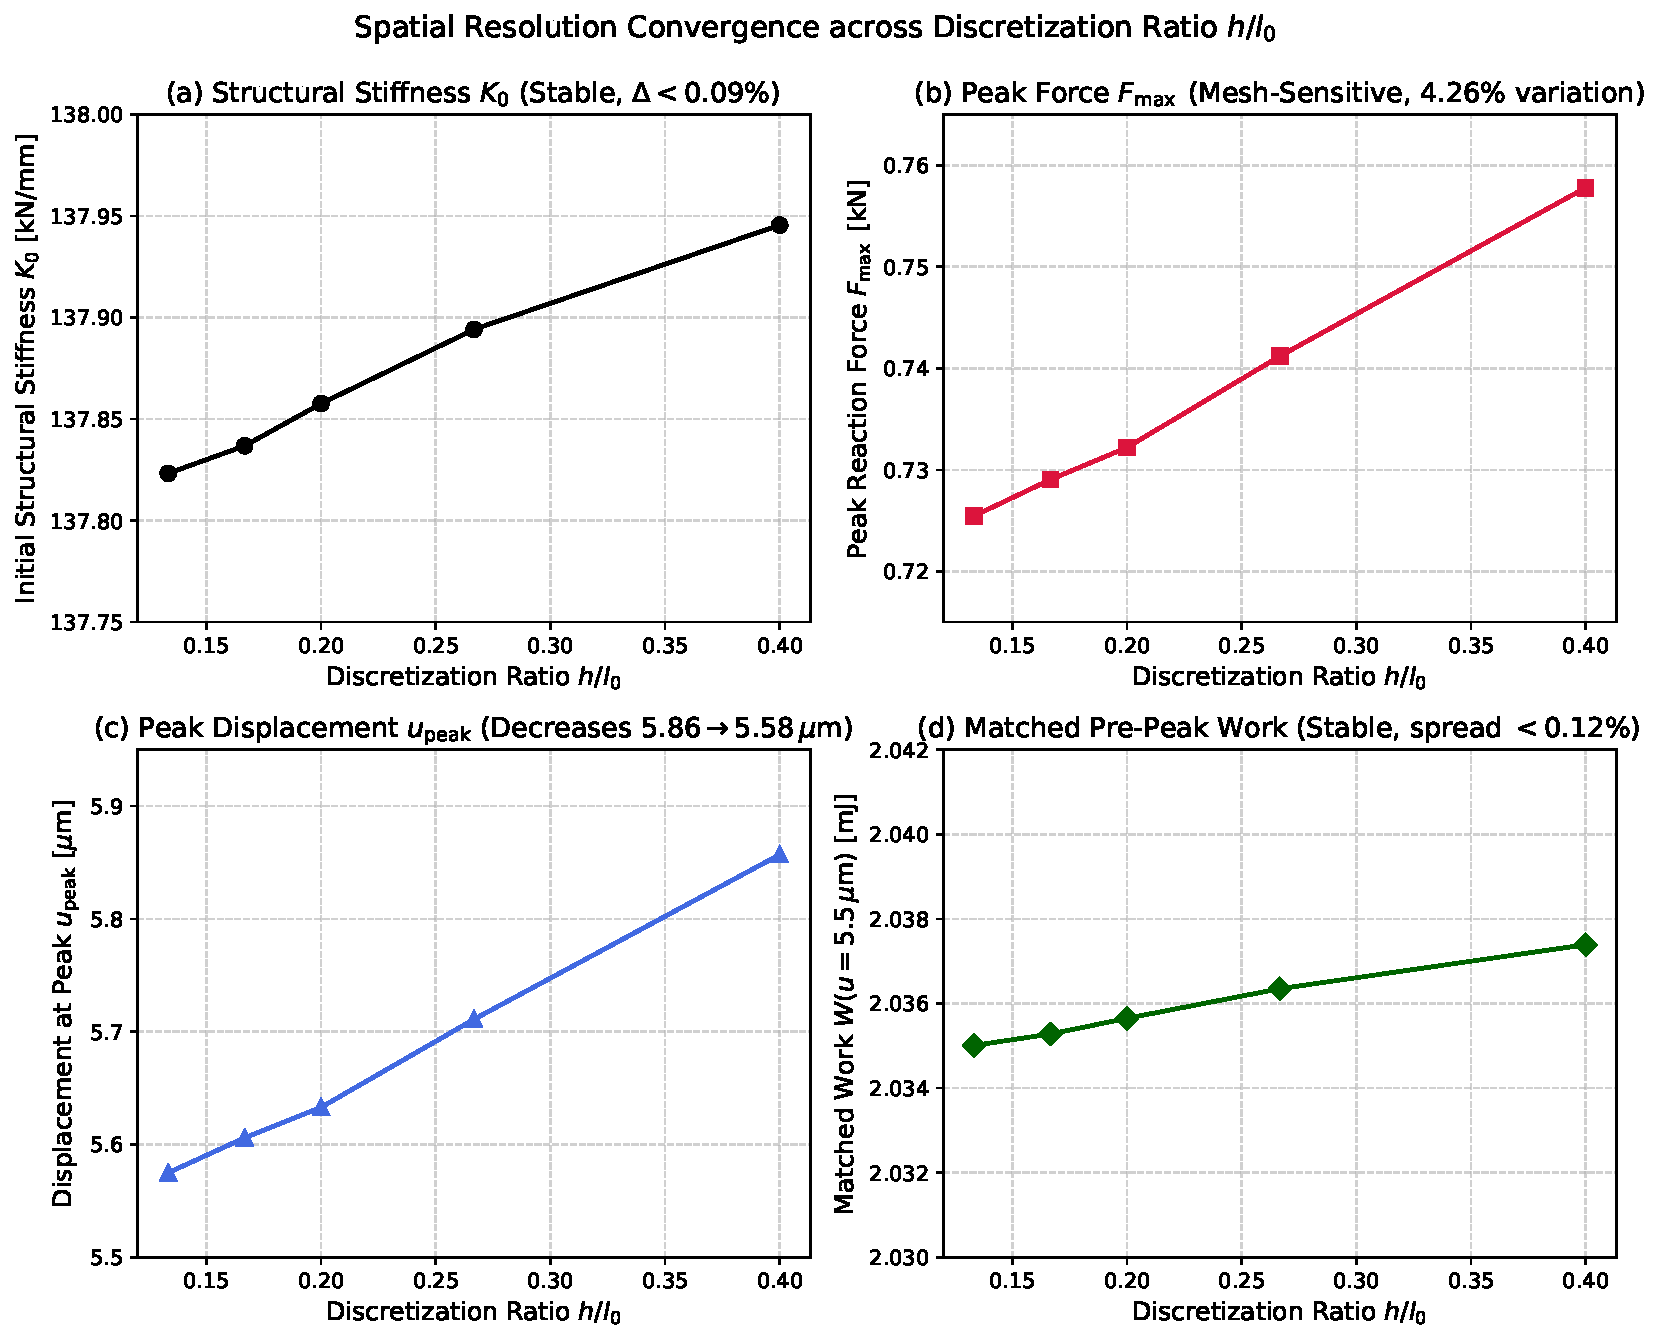
\includegraphics[width=0.92\textwidth]{fig_mode1_spatial_convergence_metrics.pdf}
  \caption{Discretization ratio ($h/l_0$) scaling metrics: (a) exceptional invariance of initial stiffness $K_0$ ($\Delta < 0.09\%$); (b) monotonic mesh sensitivity of peak force $F_{\max}$ ($4.26\%$); (c) peak displacement shift $u_{\mathrm{peak}}$; (d) matched-displacement external work $W_{\mathrm{trap}}$.}
  \label{fig:spatial_metrics_pack}
  \figureconclusion{Convergence is quantity-dependent: $K_0$ and matched pre-peak work are nearly invariant, whereas $F_{\max}$ and $u_{\mathrm{peak}}$ change systematically with $h/l_0$. The solution must not be described as fully mesh-converged.}
\end{figure}

\clearpage

\subsection{Temporal Time-Increment Scaling ($T_1$--$T_3$)}
Time incrementation was tested across three schedules at fixed baseline resolution ($h = 3.0\,\mu\mathrm{m}$): Case $T_1$ (coarse $2\times$, $3{,}500$ incs), Case $T_2$ (nominal $1\times$, $7{,}000$ incs), and Case $T_3$ (fine $0.5\times$, Job \texttt{1406317.mmaster02}, completed all $10{,}022$ Step-2 incs to $u = 10.0\,\mu\mathrm{m}$).
\begin{itemize}
  \item \textbf{Peak Mechanical Invariance:} Initial stiffness $K_0$ varies by $<0.001\%$, and peak force varies by $<0.07\%$ ($0.75815 \to 0.75763\,\mathrm{kN}$), proving temporal stability of limit loads (\textbf{\texttt{CONVERGED / STABLE}}, Fig.~\ref{fig:temporal_pack}).
  \item \textbf{Energetic Temporal Sensitivity:} Terminal trapezoidal boundary work $W_{\mathrm{trap}}$ varies by $3.24\%$ ($2.41011 \to 2.33189\,\mathrm{mJ}$), and the two-term bookkeeping difference $\mathcal{R}_{\mathrm{bookkeeping}} = W_{\mathrm{trap}} - (E_{\mathrm{elas}} + E_{\mathrm{frac}})$ shifts from $+0.378\%$ to $+3.541\%$ (\textbf{\texttt{TEMPORALLY SENSITIVE}}).
\end{itemize}

\begin{figure}[htbp]
  \centering
  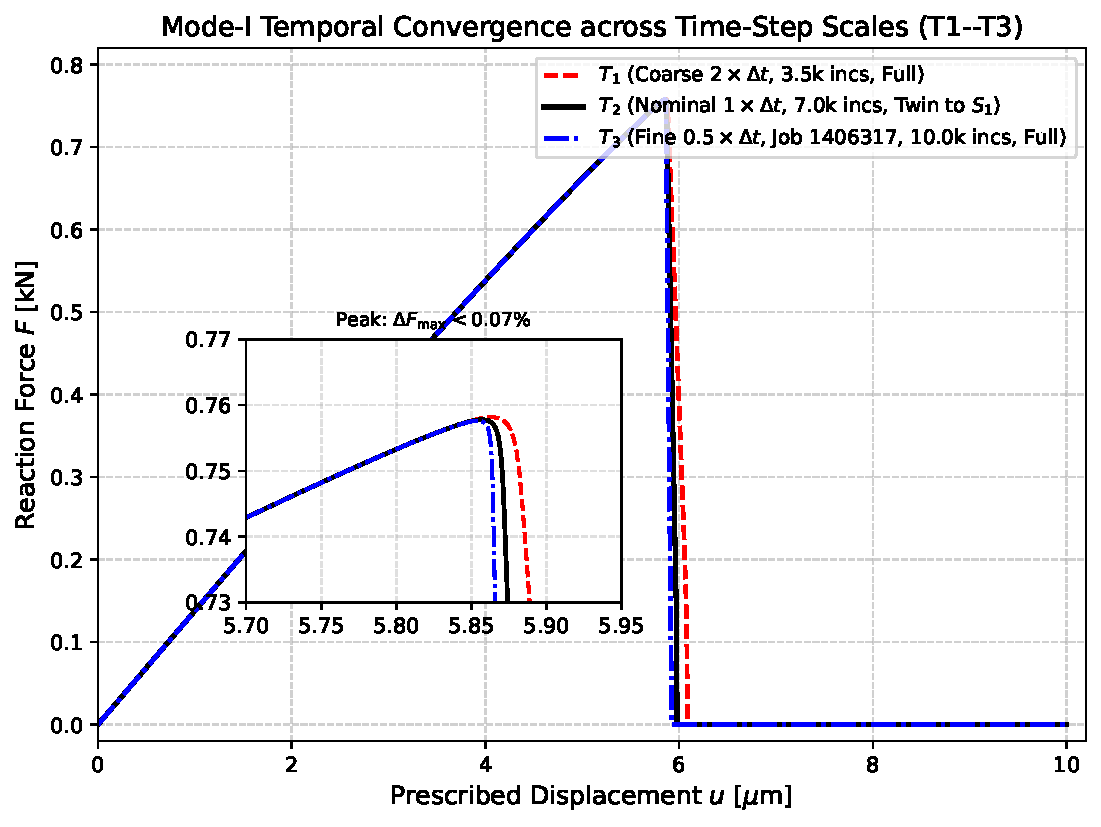
\includegraphics[width=0.78\textwidth]{fig_mode1_temporal_convergence.pdf}
  \caption{Mode-I temporal convergence across time increment scales ($T_1$: $2\times$, $T_2$: $1\times$, $T_3$: $0.5\times$, Job \texttt{1406317.mmaster02}), showing step-size invariance of the mechanical peak.}
  \label{fig:temporal_pack}
  \figureconclusion{The mechanical response through the peak is temporally converged over $T_1$--$T_3$ ($\Delta K_0<0.001\%$, $\Delta F_{\max}<0.07\%$). The spatial peak sensitivity in Fig.~\ref{fig:spatial_fu_pack} therefore cannot reasonably be attributed to insufficient time resolution; post-peak energy is assessed separately.}
\end{figure}

\clearpage

\subsection{Adaptive Remeshing Series ($A_1$--$A_4$)}
Figure~\ref{fig:adaptive_meshes_comparison_pack} displays the Abaqus-native adaptive meshes generated using `errorTarget` values of $1\%$, $2\%$, $3\%$, and $5\%$ ($A_1$--$A_4$), showing the full specimen domain and crack-tip zoom windows. As target discretization tolerance relaxes, element density smoothly transitions from intense crack-line refinement ($71{,}320$ elements) down to coarser background meshes ($4{,}194$ elements).

\begin{figure}[htbp]
  \centering
  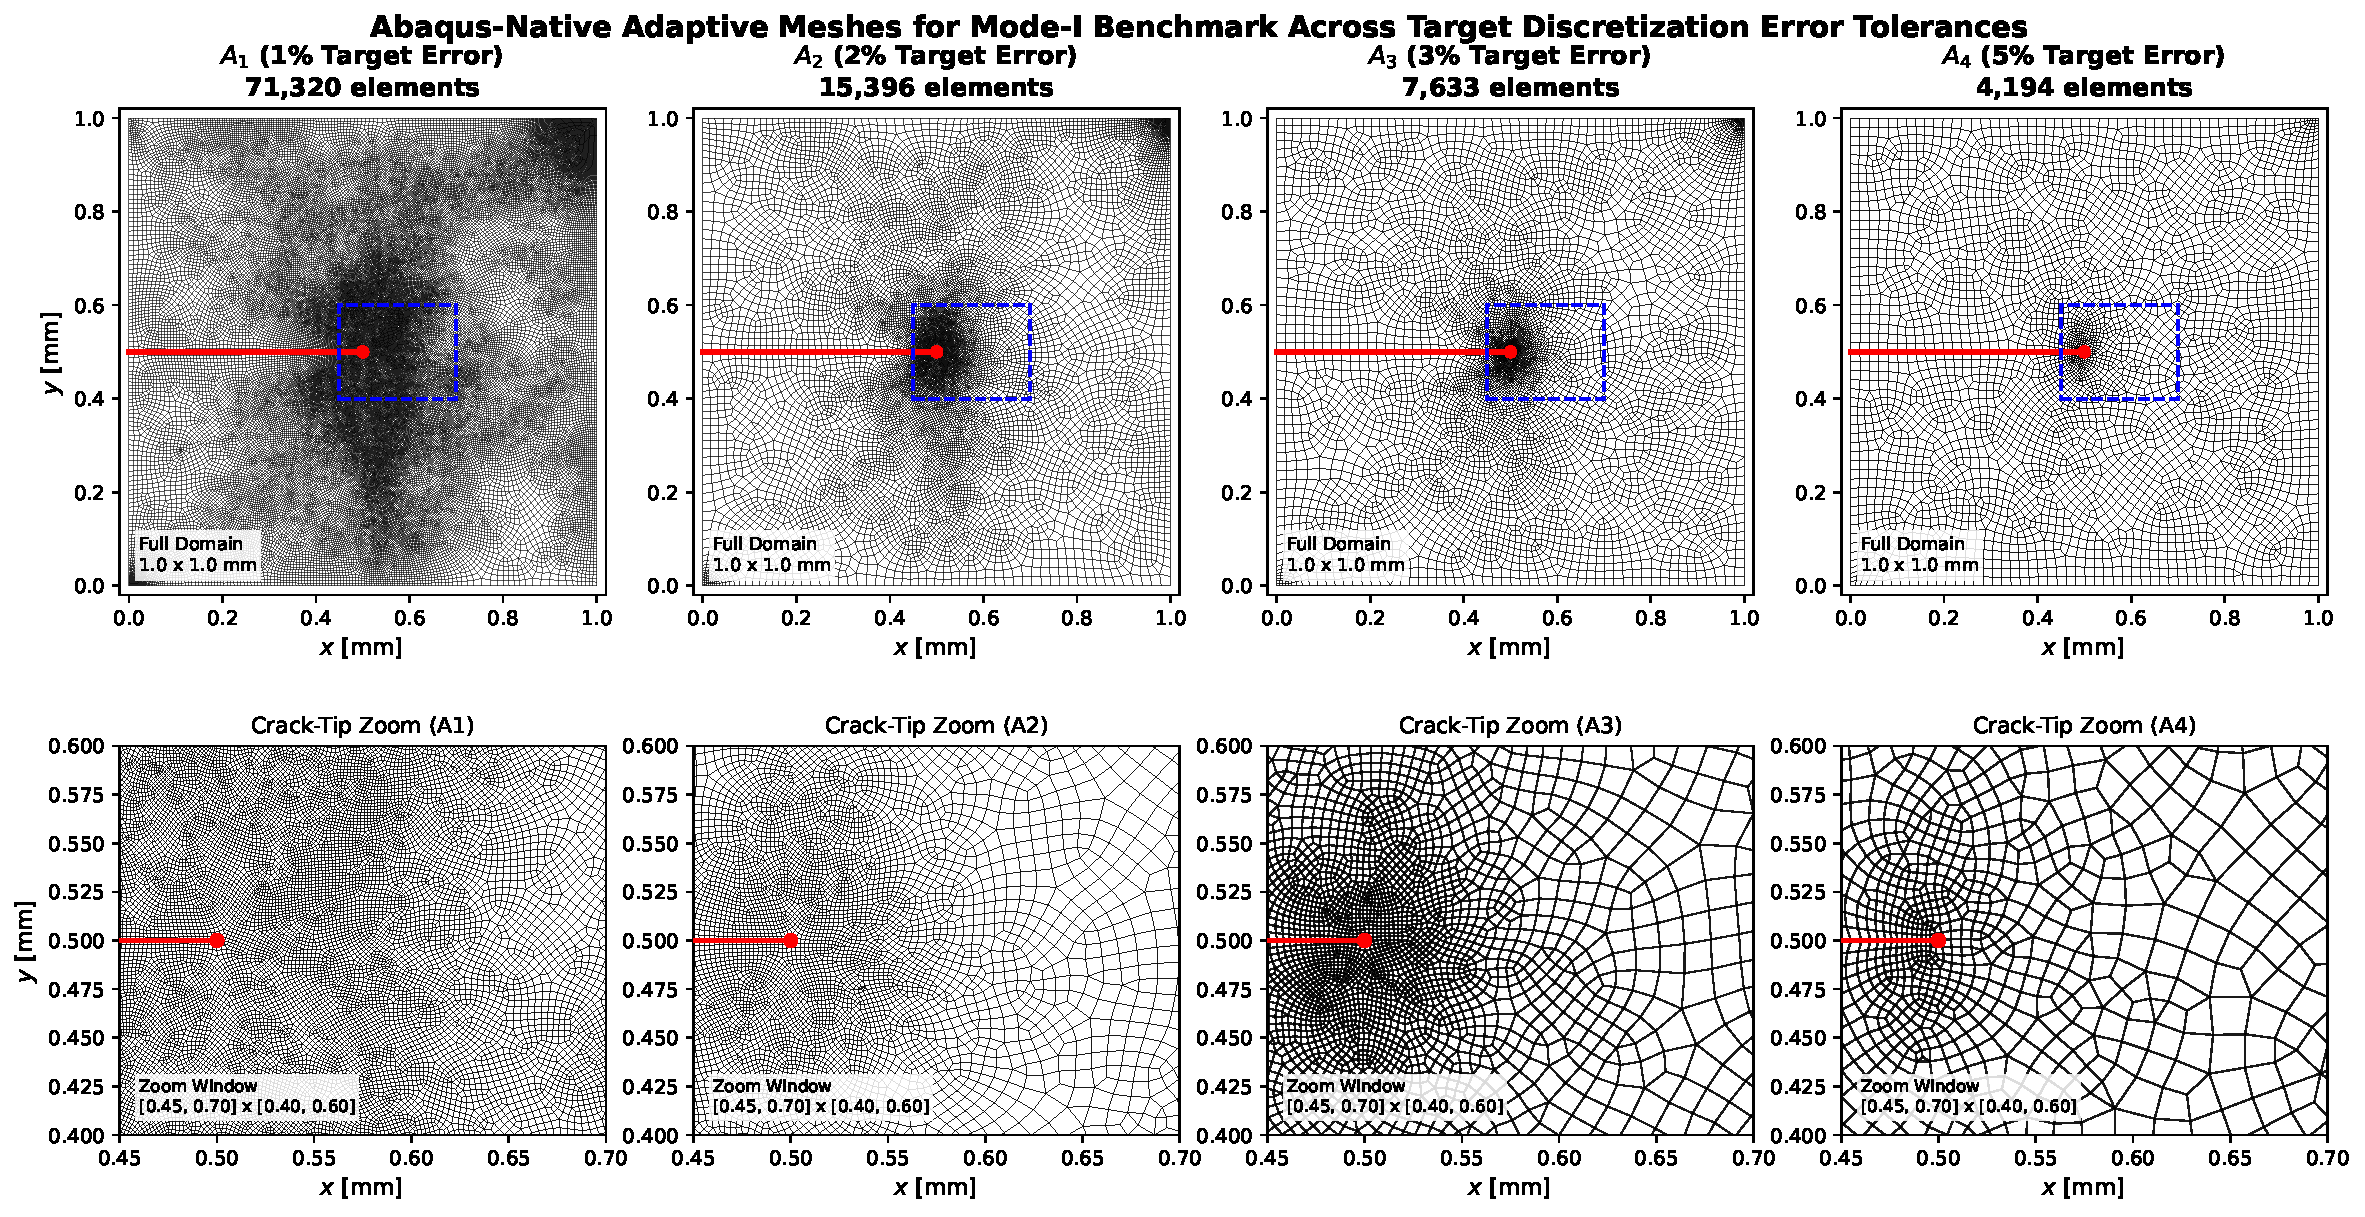
\includegraphics[width=0.98\textwidth]{fig_adaptive_meshes_comparison.pdf}
  \caption{Abaqus-native adaptive meshes generated for the Mode-I benchmark using \texttt{errorTarget} values of (a) 1\%, (b) 2\%, (c) 3\%, and (d) 5\%. The corresponding production meshes contain $71{,}320$, $15{,}396$, $7{,}633$, and $4{,}194$ underlying finite elements, respectively. Full-domain views and identical crack-tip zooms illustrate how relaxing the target error changes the spatial refinement distribution.}
  \label{fig:adaptive_meshes_comparison_pack}
  \figureconclusion{Relaxing \texttt{errorTarget} from $1\%$ to $5\%$ sharply reduces element count and progressively coarsens the crack-tip region, exposing the intended accuracy--cost trade-off of native error-controlled pre-refinement.}
\end{figure}

Figure~\ref{fig:adaptive_pack} shows the corresponding force--displacement response:
\begin{itemize}
  \item \textbf{Elastic Agreement:} All adaptive models reproduce the canonical initial stiffness $K_0 \approx 137.85\,\mathrm{kN/mm}$ within $0.09\%$.
  \item \textbf{Softening Response:} $A_1$ follows the reference softening drop up to cutback at $u = 6.77\,\mu\mathrm{m}$, while coarser meshes ($A_2$--$A_4$) reach the full $10.0\,\mu\mathrm{m}$ endpoint. Mesh $A_4$ exhibits an elevated post-peak plateau ($F \sim 0.033\,\mathrm{kN}$), classified as \textbf{\texttt{OBSERVED\_FORCE\_PLATEAU (CRACK-PINNING HYPOTHESIS / NOT YET INDEPENDENTLY PROVEN)}}.
\end{itemize}

\begin{figure}[htbp]
  \centering
  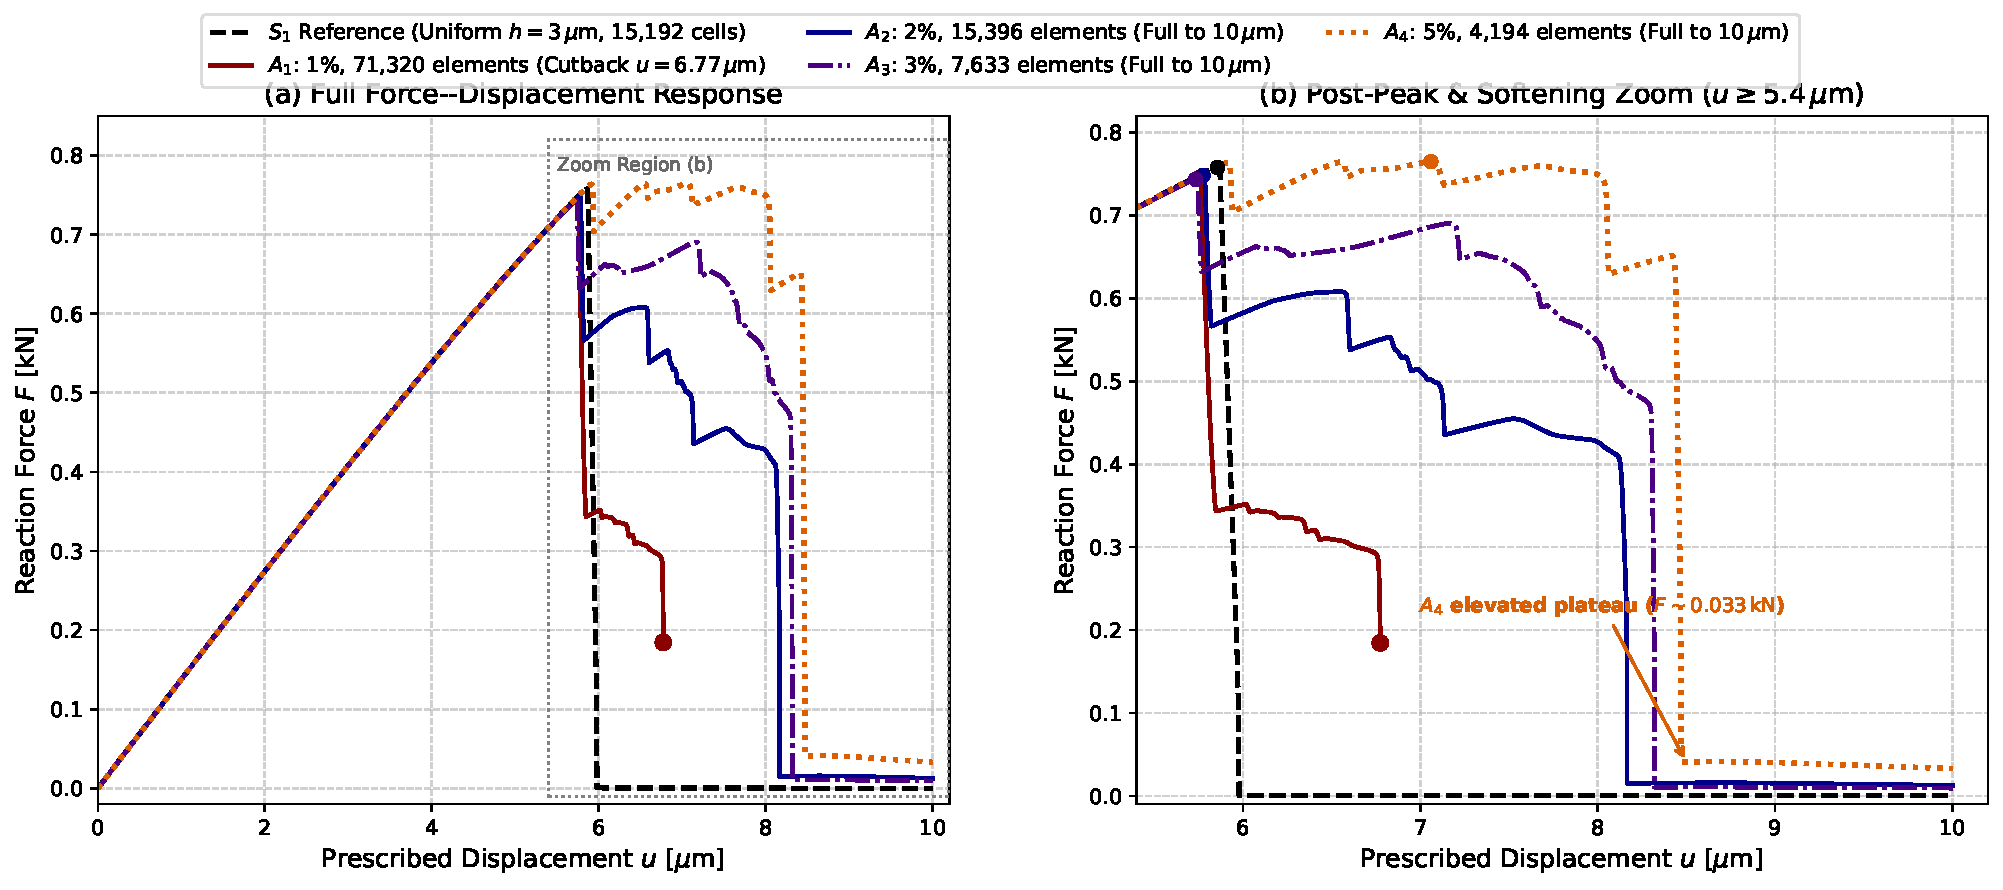
\includegraphics[width=0.98\textwidth]{fig_mode1_adaptive_convergence.pdf}
  \caption{Force--displacement response of the canonical uniform reference $S_1$ and native adaptive meshes $A_1$--$A_4$: (a) full response over $u \in [0, 10]\,\mu\mathrm{m}$; (b) post-peak zoom over $u \in [5.4, 10]\,\mu\mathrm{m}$. Production adaptive meshes contain $71{,}320$, $15{,}396$, $7{,}633$, and $4{,}194$ underlying finite elements for \texttt{errorTarget} values of 1\%, 2\%, 3\%, and 5\%, respectively. $A_1$ terminates at $u = 6.77\,\mu\mathrm{m}$, whereas $A_2$--$A_4$ reach $10\,\mu\mathrm{m}$.}
  \label{fig:adaptive_pack}
  \figureconclusion{All adaptive meshes recover the elastic stiffness, yet their initiation and post-peak responses separate substantially. Matching $K_0$ is therefore insufficient to establish fracture adequacy, and $A_1$--$A_4$ are not adaptive-tolerance-independent post peak; the $A_4$ plateau mechanism remains unproven.}
\end{figure}

\clearpage

\subsection{Phase-Field Contours, Crack Symmetry, and Localization Profiles}
Figures~\ref{fig:matched_contours_pack}--\ref{fig:path_dev_pack} separate three questions: where the crack propagates, how its centerline evolves, and how wide the diffuse localization band remains. Pre-peak profiles agree closely; near and after the peak, propagation timing and extent become resolution-dependent. Across all fixed and adaptive meshes, the centroid remains within $3.10\,\mu\mathrm{m}$ of the Mode-I symmetry line, whereas the $d\ge0.50$ band retains a resolution-sensitive full width of approximately $20$--$30\,\mu\mathrm{m}$.

\begin{figure}[htbp]
  \centering
  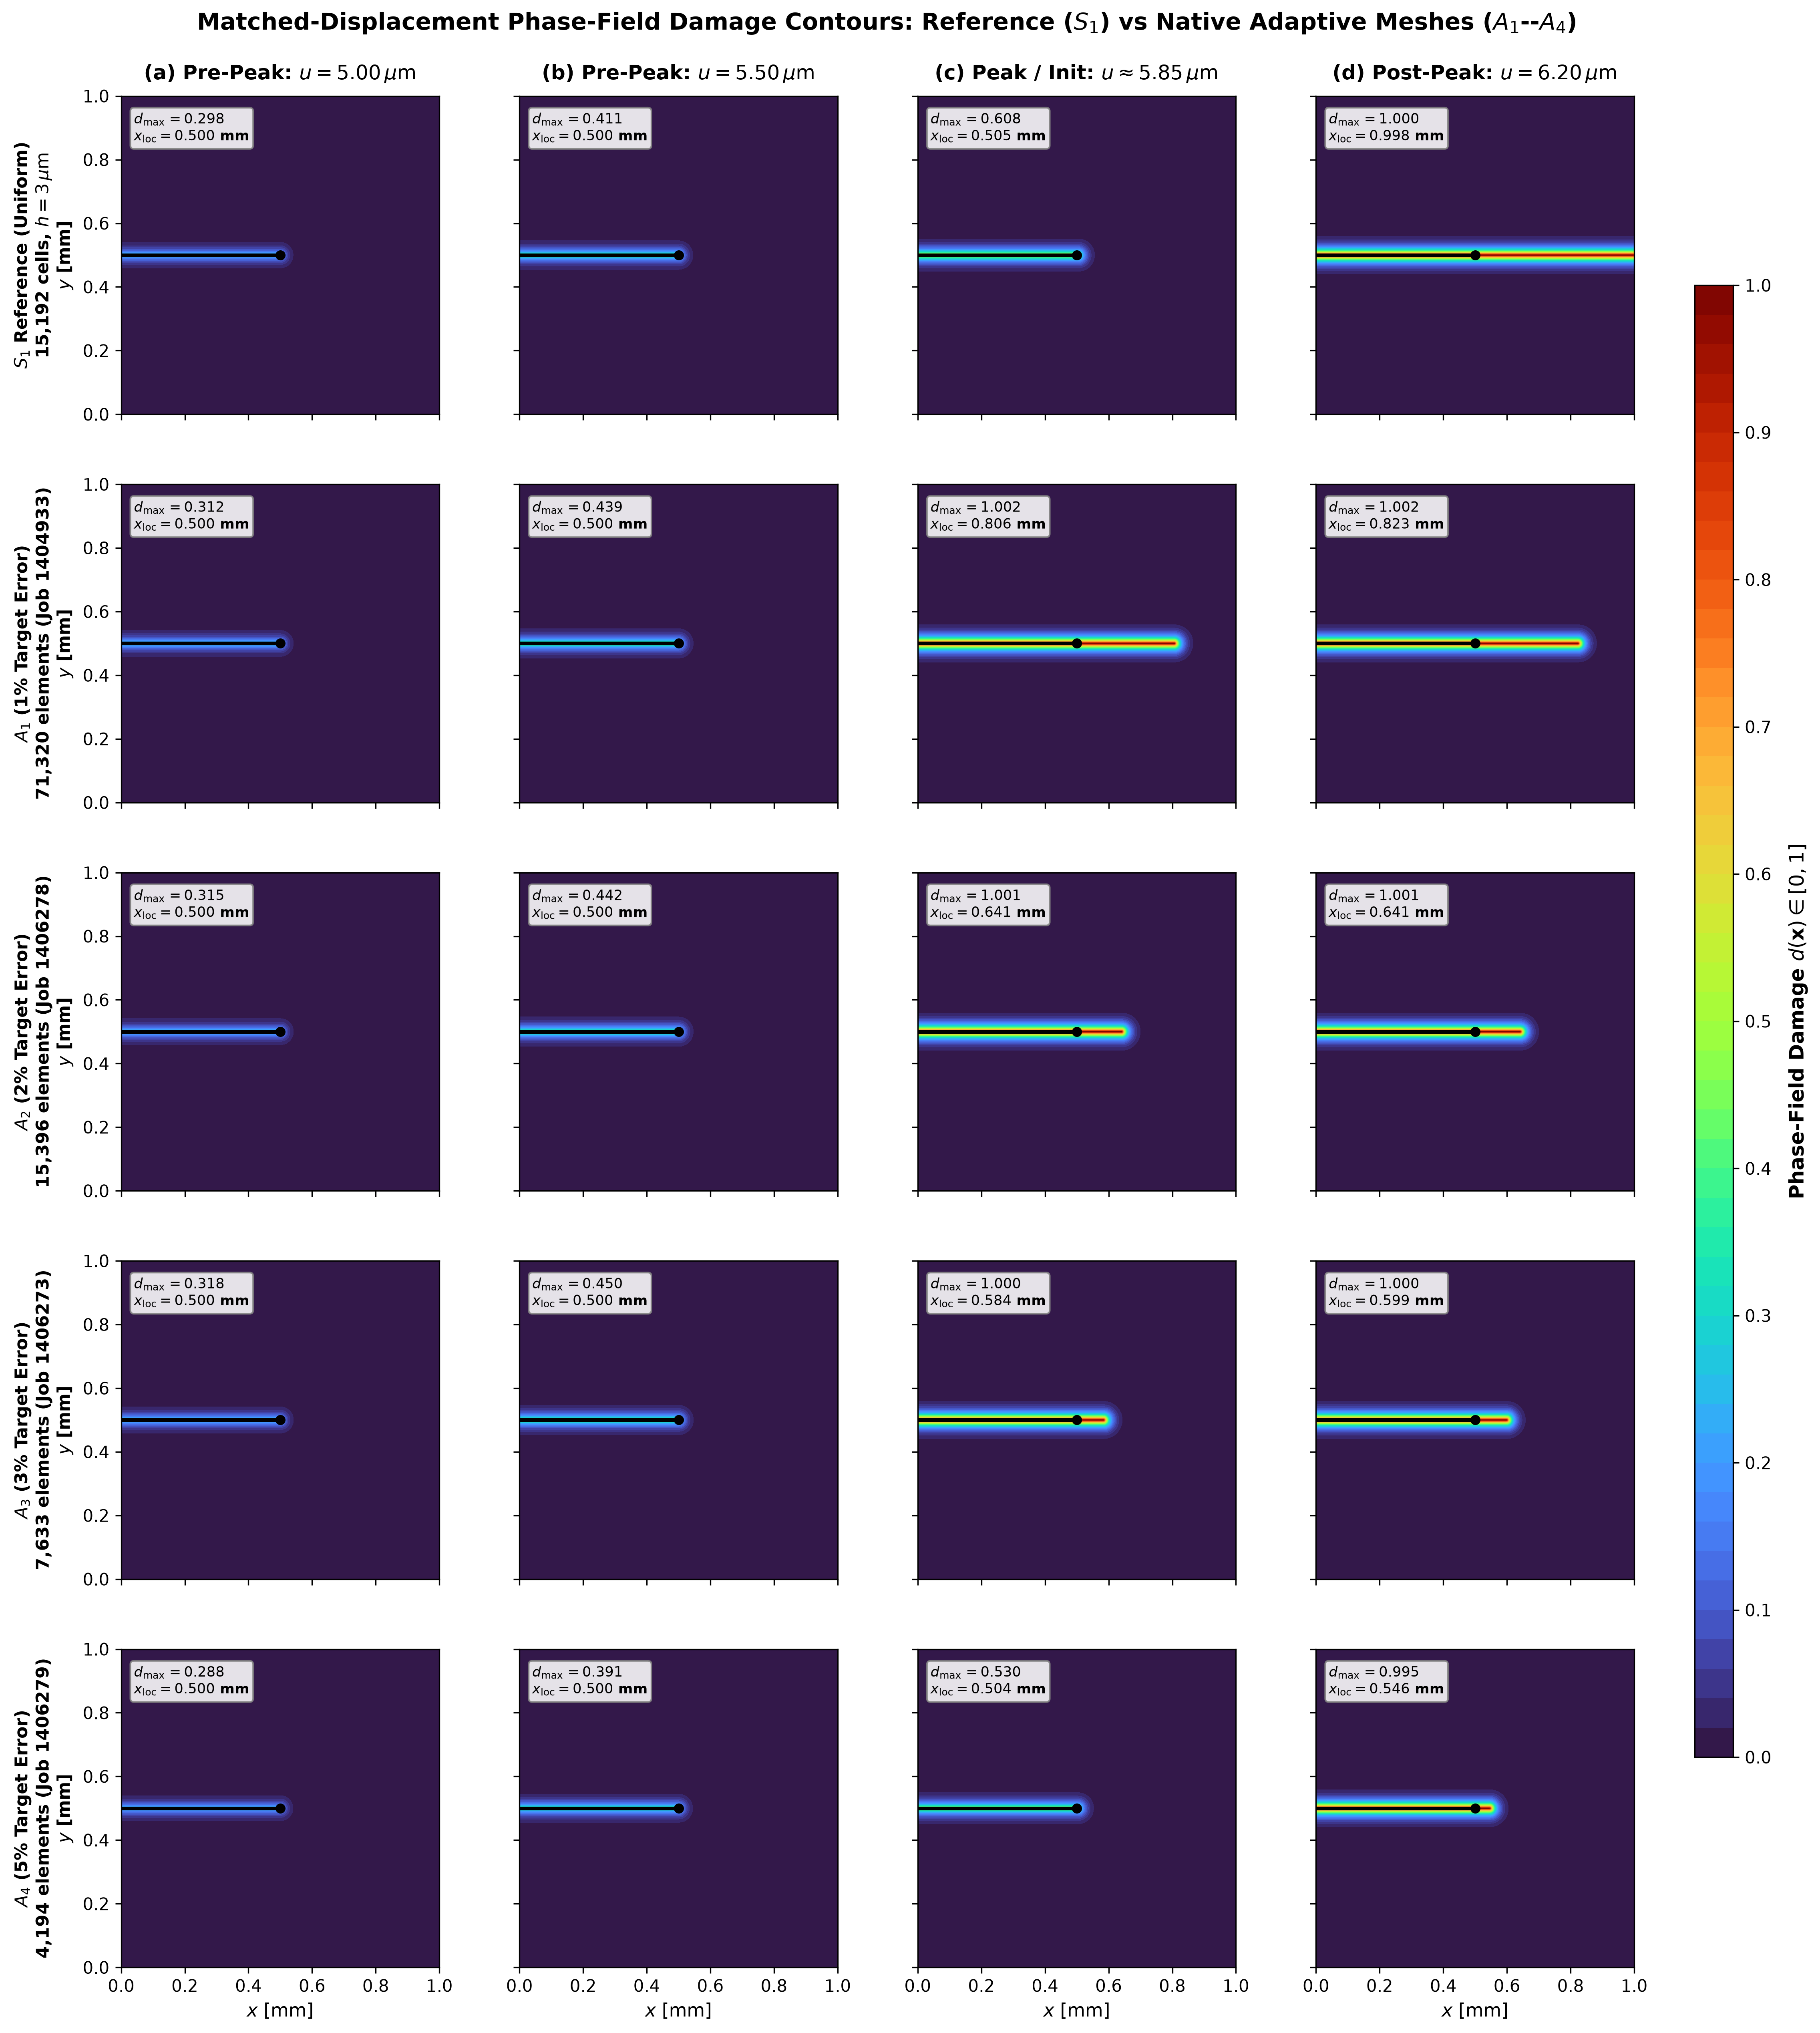
\includegraphics[width=0.88\textwidth]{gate6_matched_phase_field_contours.png}
  \caption{Matched-displacement phase-field damage contours comparing canonical reference $S_1$ ($15{,}192$ elements) and corrected native adaptive meshes $A_1$--$A_4$ across deformation states: (a) initiation at $u=5.00\,\mu\mathrm{m}$; (b) pre-peak concentration at $u=5.50\,\mu\mathrm{m}$; (c) peak / crack initiation at $u\approx 5.85\,\mu\mathrm{m}$; (d) post-peak propagated crack at $u=6.20\,\mu\mathrm{m}$.}
  \label{fig:matched_contours_pack}
  \figureconclusion{Pre-peak localization is broadly consistent, while crack-propagation timing and extent become resolution-dependent near and after the peak. The propagation direction nevertheless remains robustly aligned with the horizontal Mode-I path.}
\end{figure}

\begin{figure}[htbp]
  \centering
  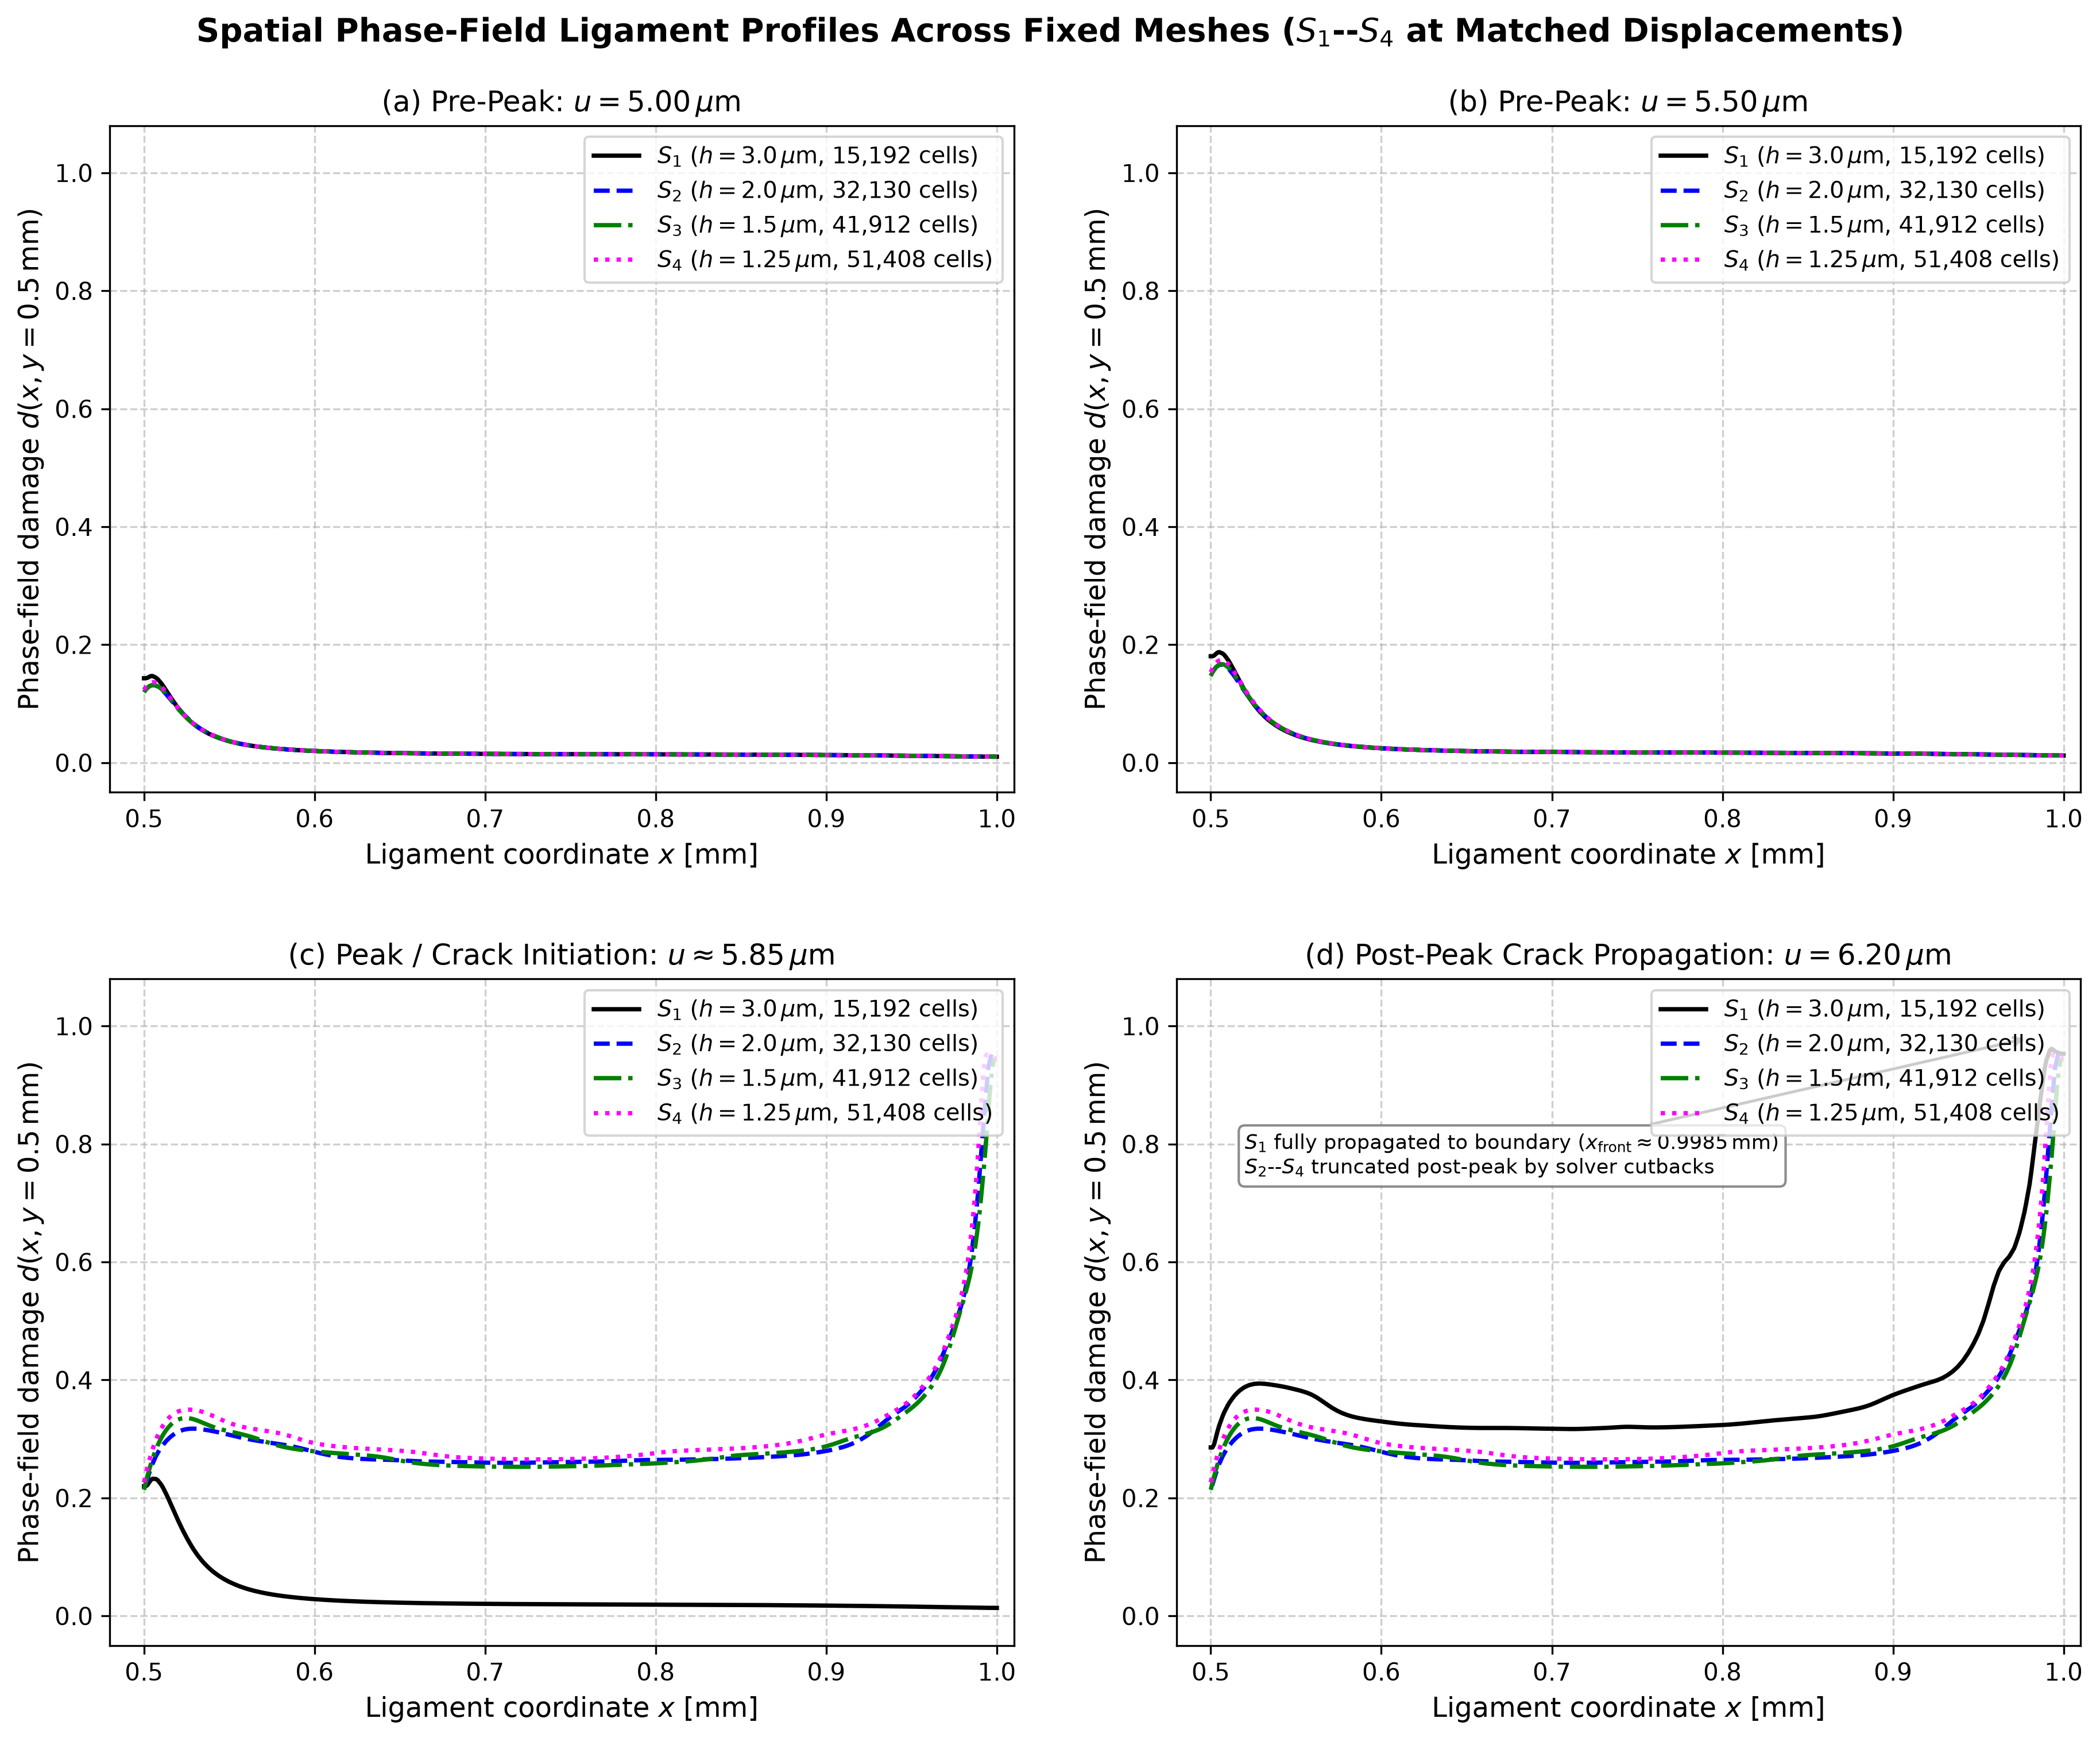
\includegraphics[width=0.88\textwidth]{fig1_fixed_mesh_ligament_profiles.png}
  \caption{Spatial phase-field ligament profiles $d(x, y=0.5\,\mathrm{mm})$ for fixed meshes $S_1$--$S_4$ across matched displacement levels, showing x-axis coordinates on all panels and annotating full boundary propagation in $S_1$ at $u = 6.20\,\mu\mathrm{m}$.}
  \label{fig:ligament_fixed_pack}
  \figureconclusion{Fixed meshes agree closely before peak loading. Near peak they separate because crack initiation occurs at different imposed displacements, and post-peak propagation extent differs; pre-peak localization is relatively stable, while near/post-peak evolution is mesh-sensitive.}
\end{figure}

\begin{figure}[htbp]
  \centering
  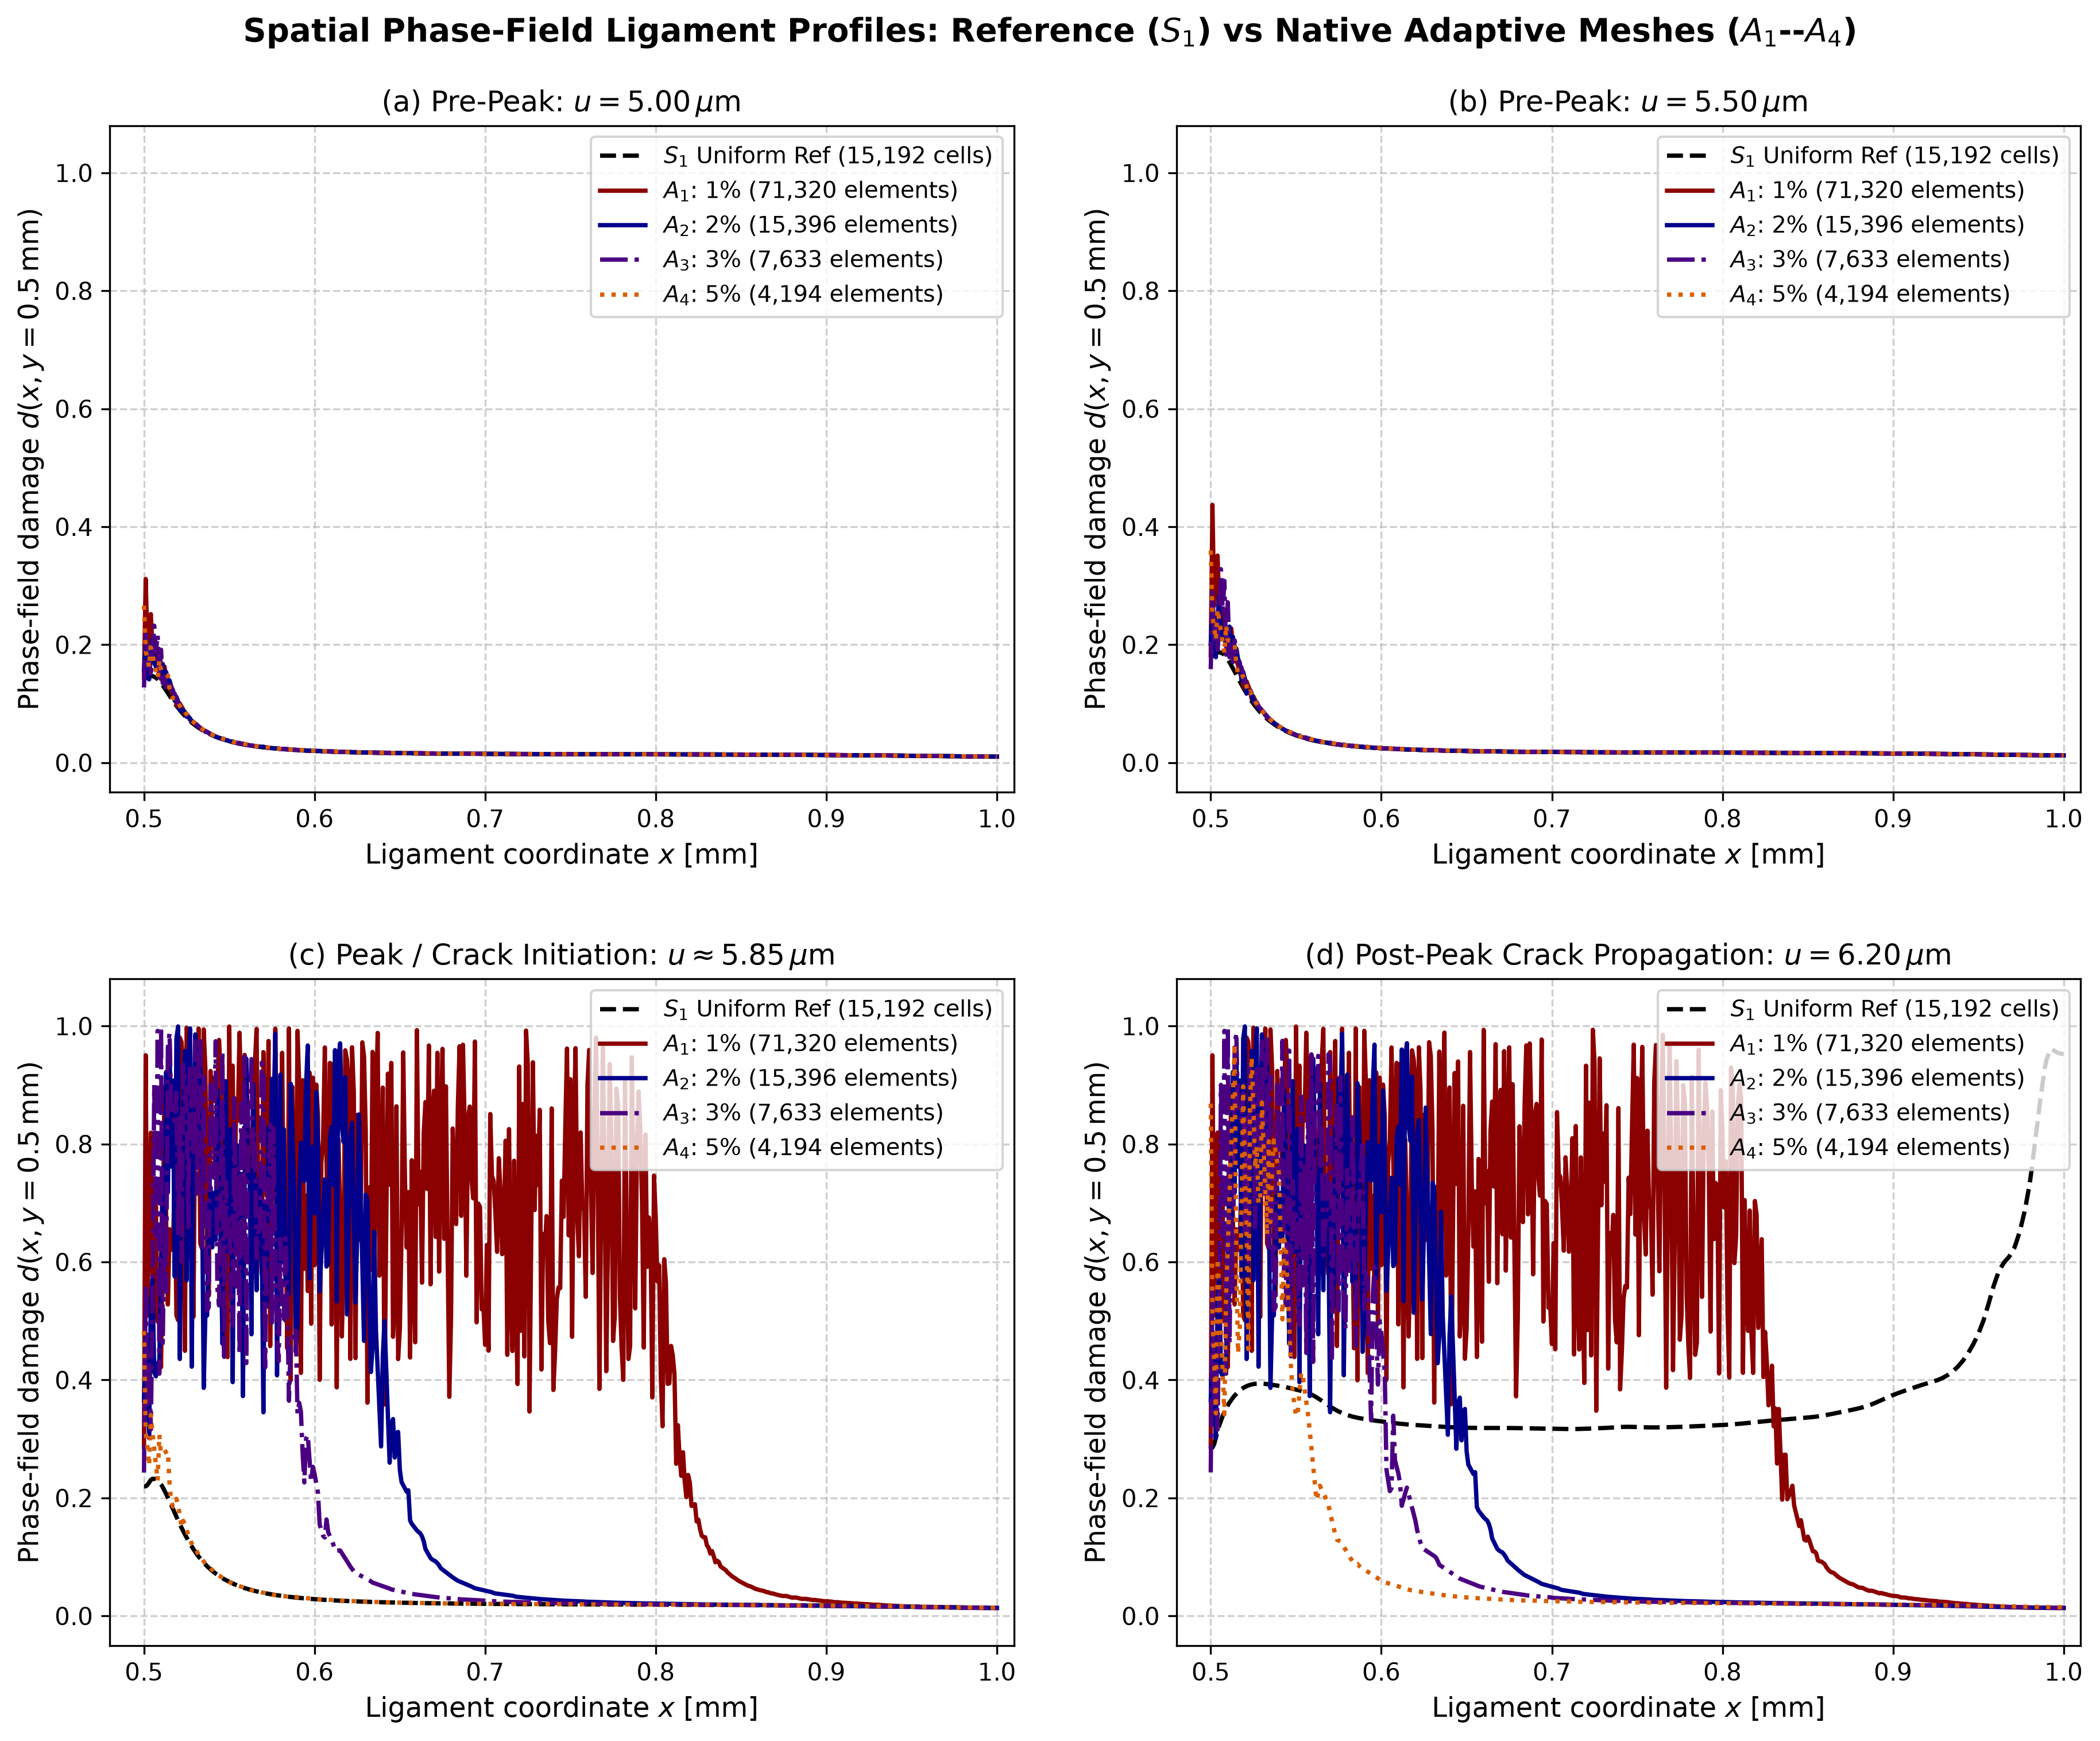
\includegraphics[width=0.88\textwidth]{fig2_adaptive_mesh_ligament_profiles.png}
  \caption{Spatial phase-field ligament profiles $d(x, y=0.5\,\mathrm{mm})$ comparing canonical reference $S_1$ against native adaptive meshes $A_1$--$A_4$ across matched displacement levels.}
  \label{fig:ligament_adaptive_pack}
  \figureconclusion{Adaptive pre-refinement reproduces the reference damage distribution reasonably well before the peak but diverges during crack initiation and unstable propagation. Post-peak crack evolution is therefore sensitive to the adaptive discretization.}
\end{figure}

\begin{figure}[htbp]
  \centering
  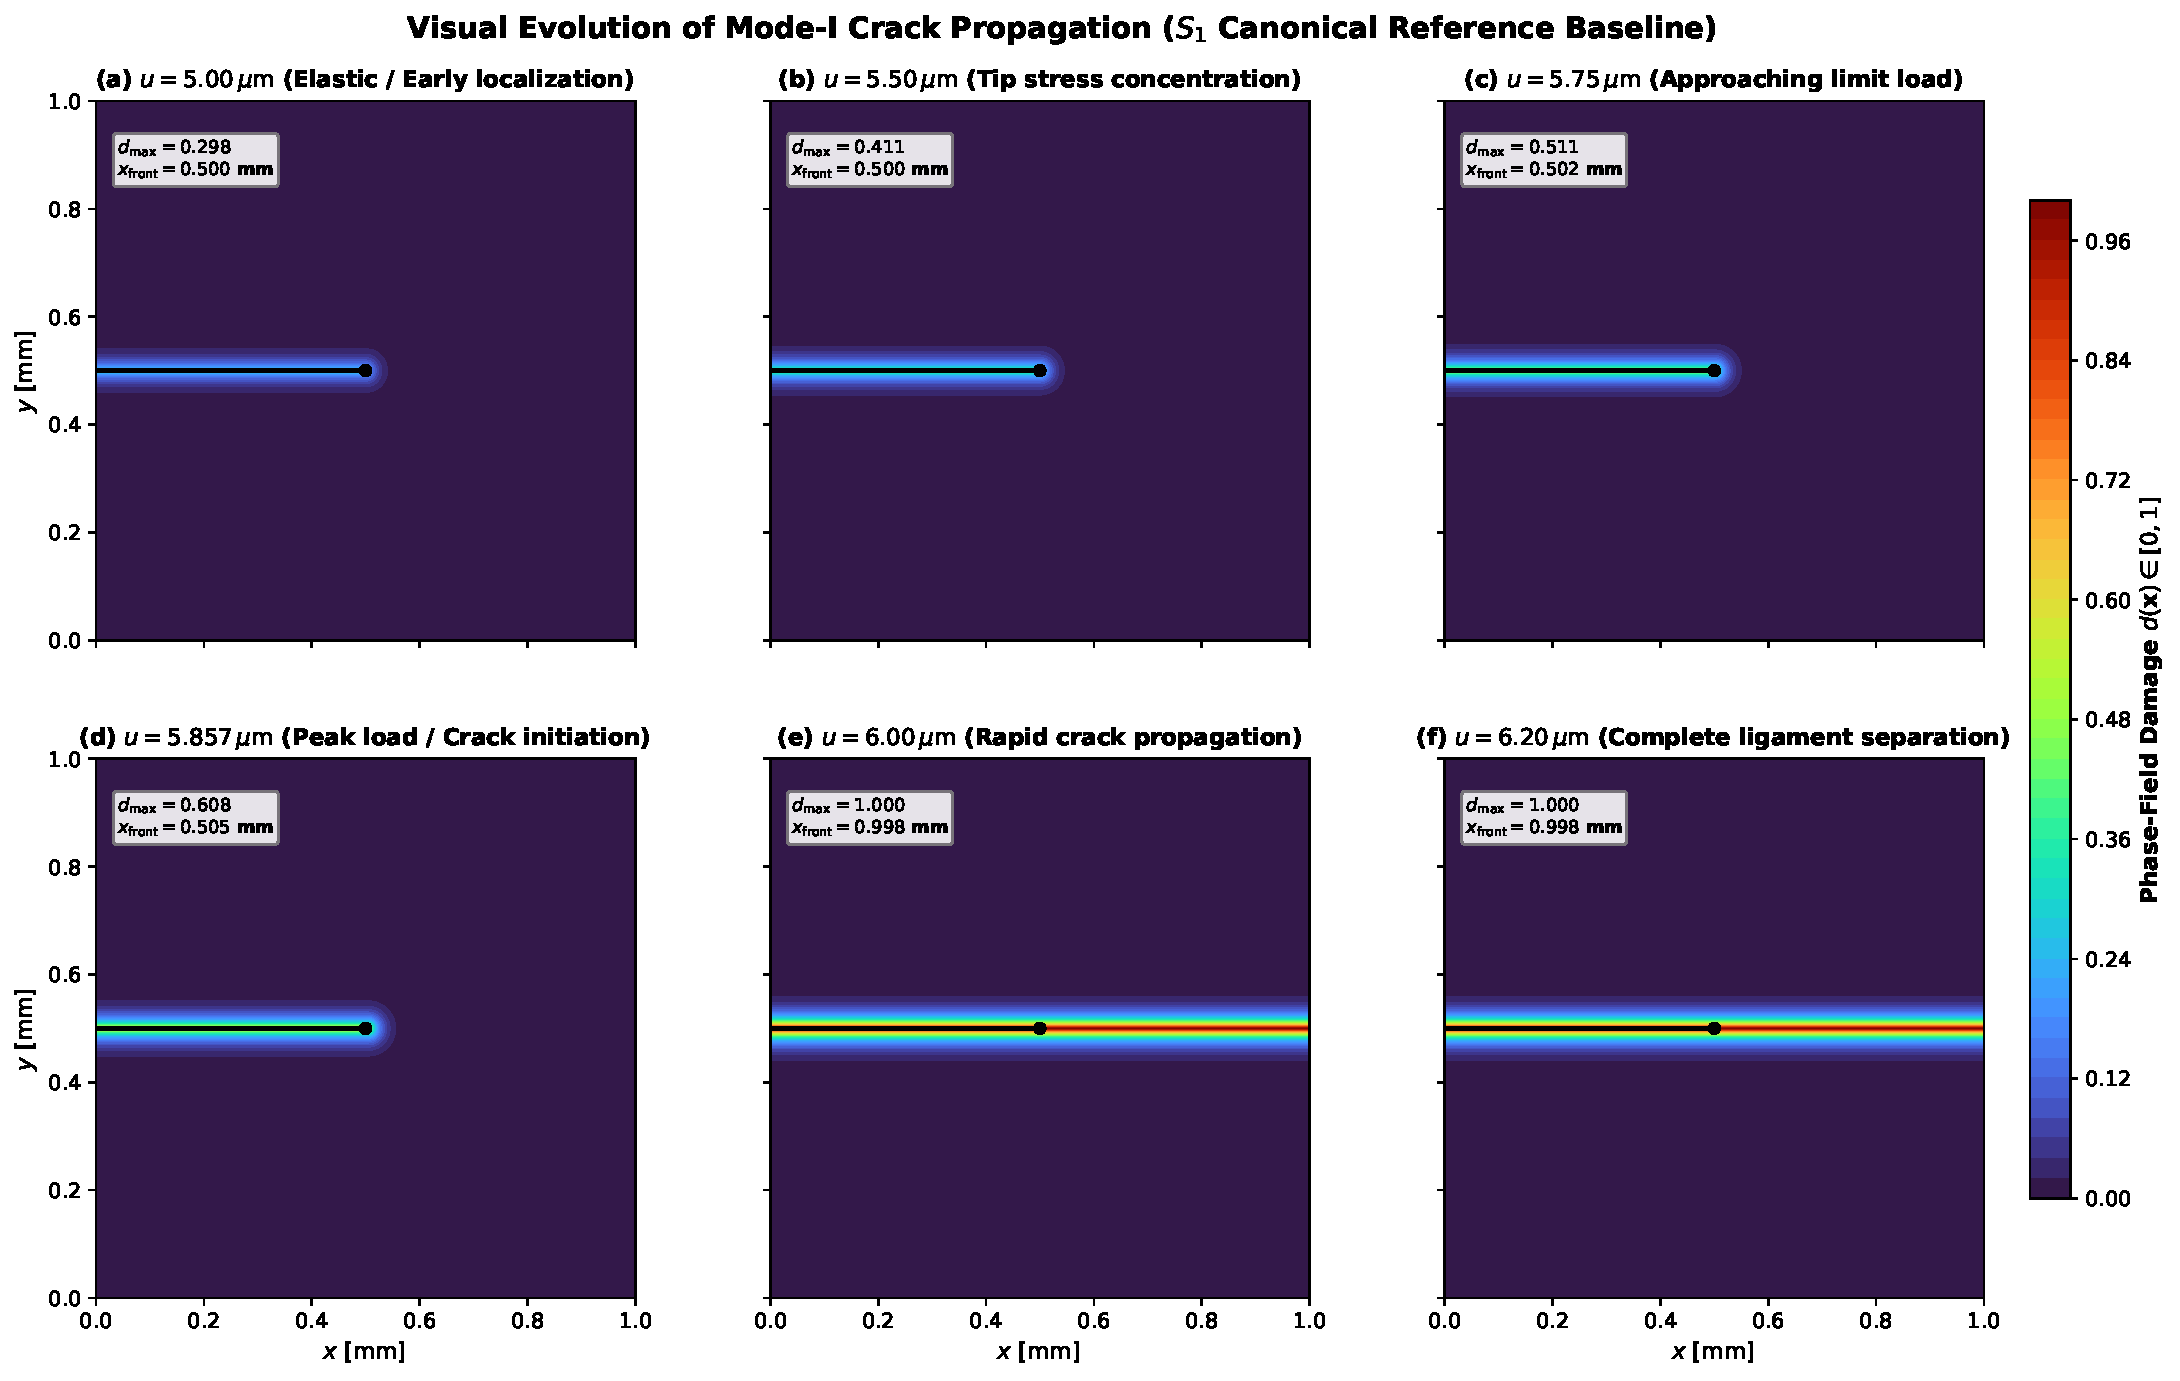
\includegraphics[width=0.92\textwidth]{fig_mode1_crack_propagation_sequence.pdf}
  \caption{Visual evolution of Mode-I crack propagation for the canonical $S_1$ reference baseline: six-stage sequence from initial elastic localization ($u = 5.0\,\mu\mathrm{m}$) through peak load ($u = 5.857\,\mu\mathrm{m}$) to complete ligament separation ($u = 6.20\,\mu\mathrm{m}$).}
  \label{fig:crack_sequence_pack}
  \figureconclusion{The canonical solution follows the expected Mode-I sequence: crack-tip localization, growth toward the limit load, initiation near the peak, rapid horizontal propagation, and complete ligament separation.}
\end{figure}

\begin{figure}[htbp]
  \centering
  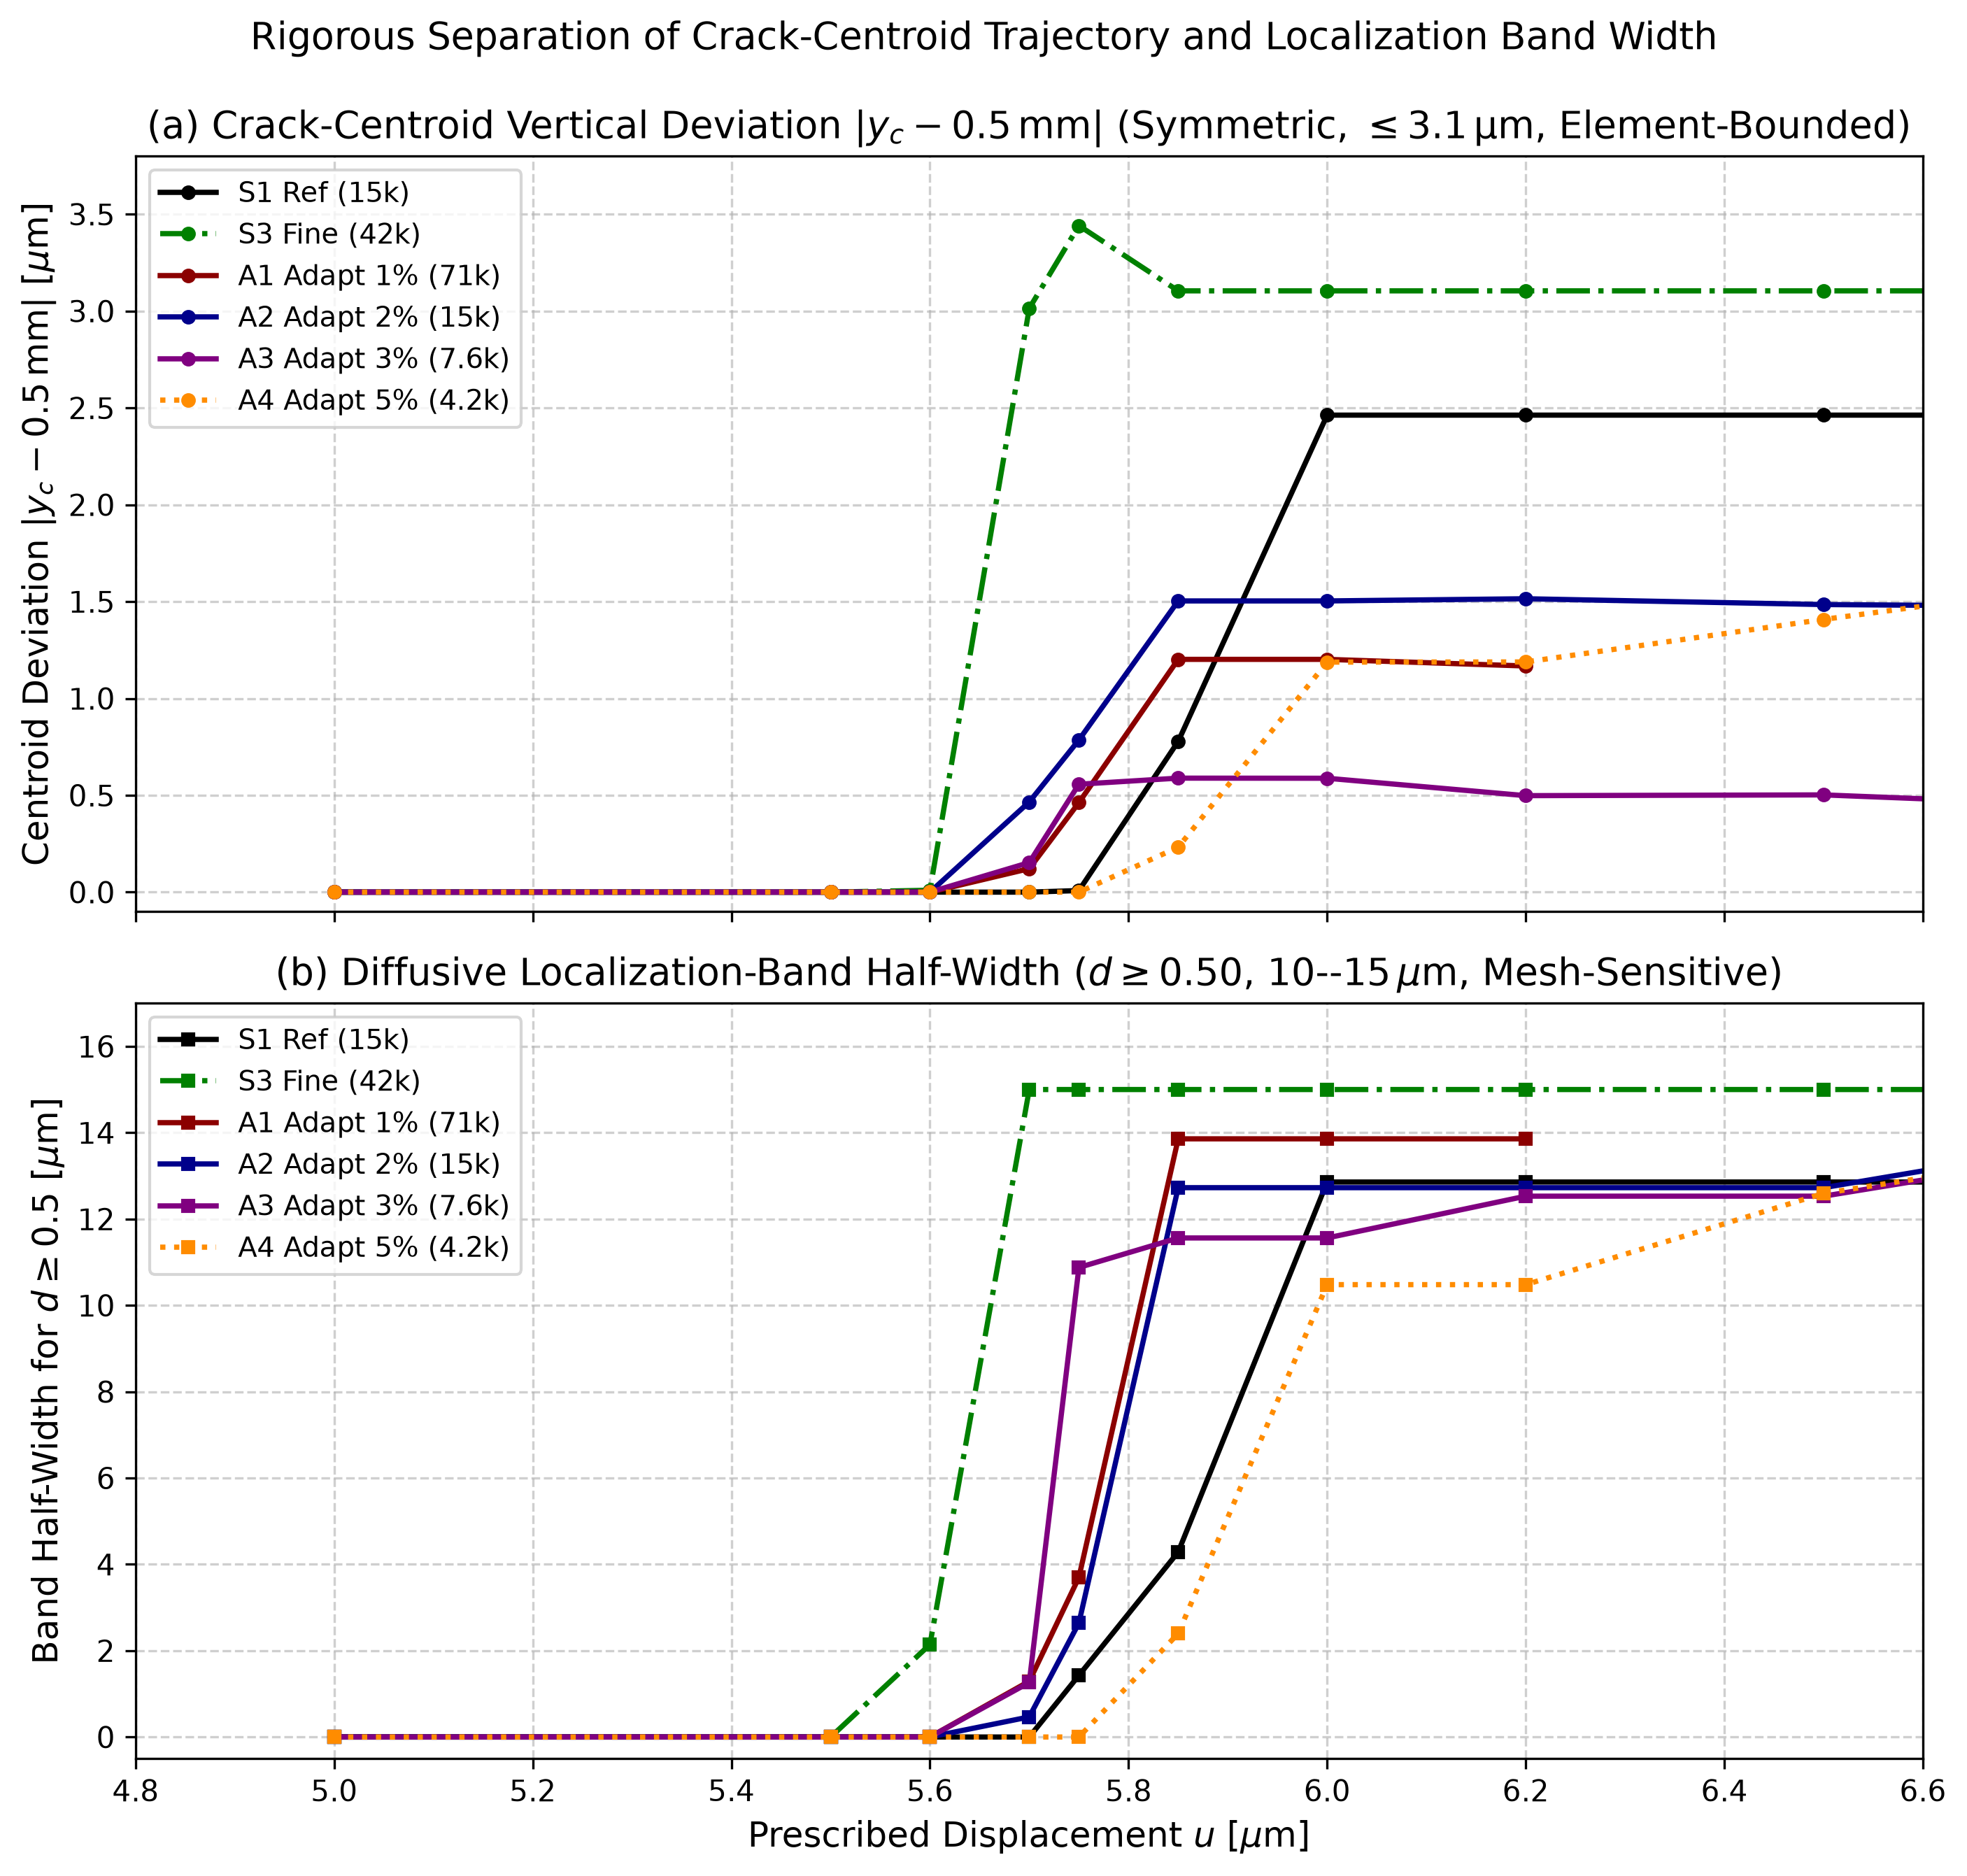
\includegraphics[width=0.78\textwidth]{fig4_vertical_path_localization_deviation.png}
  \caption{Rigorous separation of (a) damage-weighted crack-centroid offset versus prescribed displacement ($|y_c - 0.5| \le 3.1\,\mu\mathrm{m}$, symmetric) and (b) damage localization-band half-width ($10$--$15\,\mu\mathrm{m}$, resolution-limited).}
  \label{fig:path_dev_pack}
  \figureconclusion{The crack trajectory remains essentially centered and is robustly Mode-I, whereas the thickness of the diffuse localization band remains resolution-sensitive. Crack direction and band width therefore exhibit different convergence behavior.}
\end{figure}

\clearpage

\subsection{Three-Point Physical Length-Scale Study ($l_0$ on Fixed $S_3$ Mesh)}
A controlled physical length-scale study was executed on the fixed $S_3$ mesh ($h = 1.5\,\mu\mathrm{m}$, $41{,}912$ finite elements, ensuring $h/l_0 \le 0.200$) across three regularization lengths $l_0 \in \{7.5, 11.25, 15.0\}\,\mu\mathrm{m}$ (Table~\ref{tab:l0_study_pack}, Fig.~\ref{fig:l0_metrics_pack}):
\begin{itemize}
  \item \textbf{Stiffness Invariance:} Initial structural stiffness $K_0$ varies from $137.857608$ to $137.676175\,\mathrm{kN/mm}$ ($\Delta = 0.13\%$), classified as \textbf{\texttt{INSENSITIVE / STABLE OVER TESTED RANGE}}.
  \item \textbf{Peak Force and Displacement Sensitivity:} Peak reaction force drops from $0.732196\,\mathrm{kN}$ ($l_0 = 7.5\,\mu\mathrm{m}$) to $0.689540\,\mathrm{kN}$ ($l_0 = 15.0\,\mu\mathrm{m}$, a $5.83\%$ reduction), while displacement at peak shifts from $5.633\,\mu\mathrm{m}$ to $5.579\,\mu\mathrm{m}$, classified as \textbf{\texttt{LENGTH-SCALE SENSITIVE}}.
  \item \textbf{Scope Limitation:} The $l_0 = 3.75\,\mu\mathrm{m}$ case ($h/l_0 = 0.400$) is excluded as under-resolved. Terminal energy comparison across the three cases is classified as \textbf{\texttt{NOT\_YET\_QUALIFIED\_UNEQUAL\_ENDPOINTS}}.
\end{itemize}

\begin{table}[htbp]
\centering
\caption{Three-point physical length-scale sensitivity metrics on fixed $S_3$ mesh ($h = 1.5\,\mu\mathrm{m}$).}
\label{tab:l0_study_pack}
\small
\begin{tabular}{lrrrrrr}
\toprule
$l_0$ [$\mu\mathrm{m}$] & Job ID & $h/l_0$ & Elements & $K_0$ [kN/mm] & $F_{\max}$ [kN] & $u_{\mathrm{peak}}$ [$\mu\mathrm{m}$] \\
\midrule
$7.50$ & \texttt{1406017.mmaster02} & $0.200$ & $41{,}912$ & $137.857608$ & $0.732196$ & $5.633$ \\
$11.25$ & \texttt{1406895.mmaster02} & $0.133$ & $41{,}912$ & $137.765563$ & $0.708402$ & $5.590$ \\
$15.00$ & \texttt{1406896.mmaster02} & $0.100$ & $41{,}912$ & $137.676175$ & $0.689540$ & $5.579$ \\
\bottomrule
\end{tabular}
\end{table}

\begin{figure}[htbp]
  \centering
  \begin{minipage}{0.48\textwidth}
    \centering
    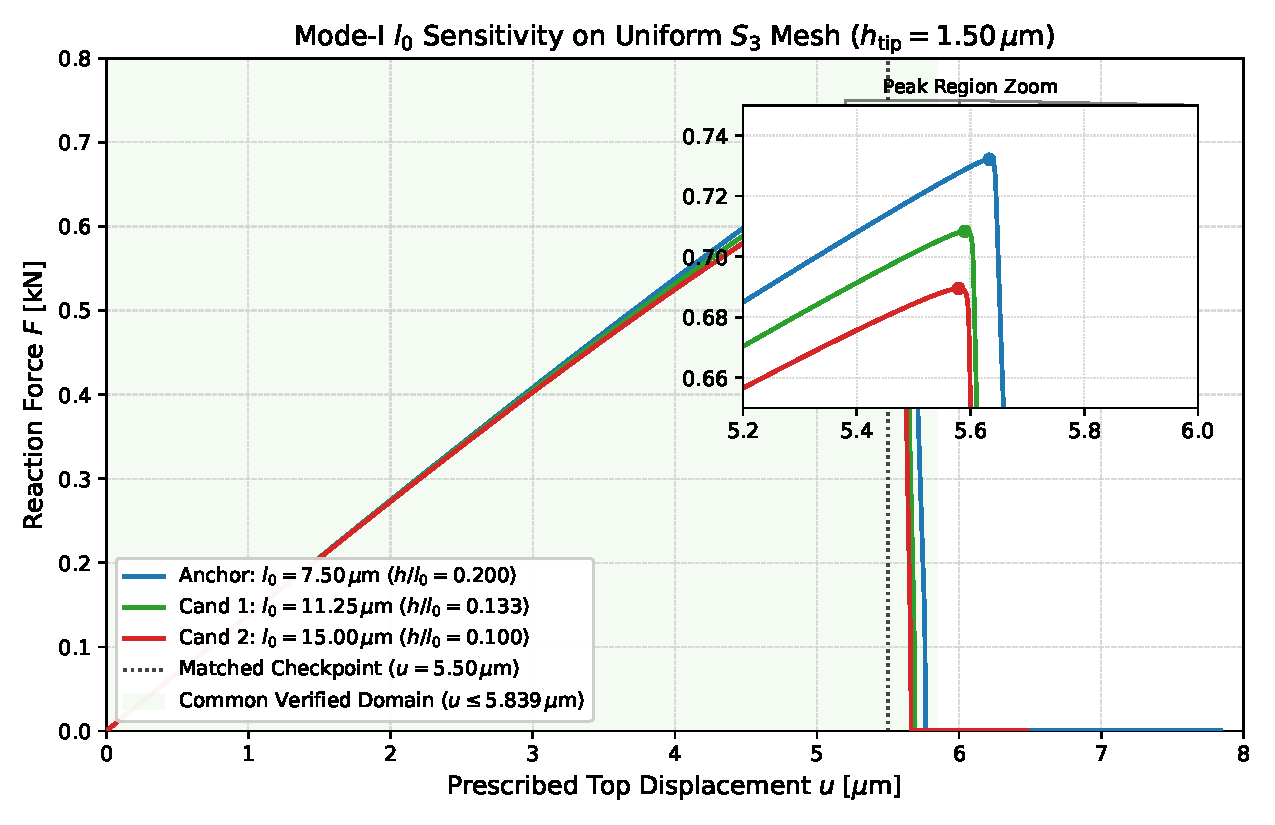
\includegraphics[width=\textwidth]{fig_mode1_l0_fu_overlay.pdf}
    \caption*{(a) $F$--$u$ response across $l_0$}
  \end{minipage}\hfill
  \begin{minipage}{0.48\textwidth}
    \centering
    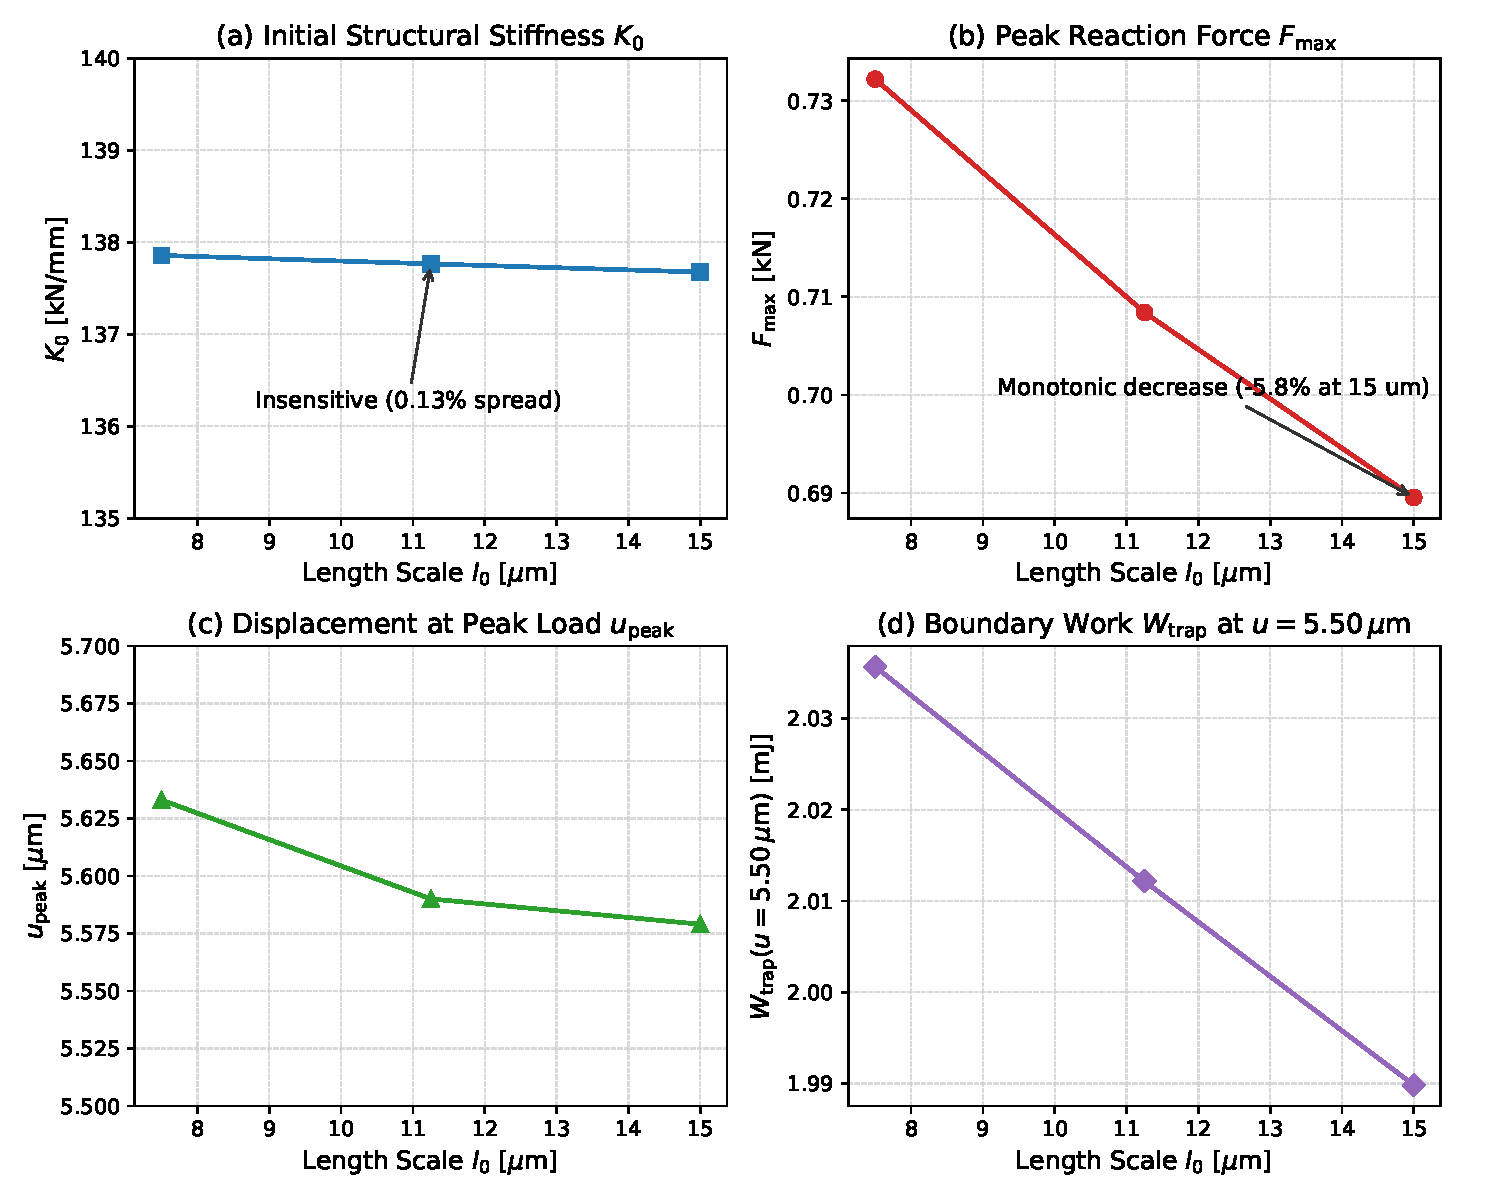
\includegraphics[width=\textwidth]{fig_mode1_l0_metrics_vs_lengthscale.pdf}
    \caption*{(b) Peak metrics vs.\ $l_0$}
  \end{minipage}
  \caption{Three-point physical length-scale study on fixed $S_3$ mesh ($h = 1.5\,\mu\mathrm{m}$): (a) global force-displacement overlay and (b) variation of $K_0$, $F_{\max}$, $u_{\mathrm{peak}}$, and matched $W_{\mathrm{trap}}$ at $u = 5.50\,\mu\mathrm{m}$ with $l_0$.}
  \label{fig:l0_metrics_pack}
  \figureconclusion{Changing $l_0$ leaves elastic stiffness nearly unchanged ($0.13\%$ spread) but materially lowers $F_{\max}$ and advances $u_{\mathrm{peak}}$. Elastic response is nearly length-scale-insensitive, while fracture initiation is physically length-scale-sensitive; terminal energies are not compared because endpoints differ.}
\end{figure}

\clearpage

\section{UEL Energy Formulation and Global Energy Balance Audit}
\label{sec:uel_energy_and_balance_audit}

\subsection{Implemented Discrete Energy Formulations and Weak-Form Derivation}
In user subroutine \nolinkurl{f42_mixed_uel.for} (SHA-256 \texttt{5cd0d2c015...}), stored elastic strain energy $E_{\mathrm{elas}}$ and fracture surface energy $E_{\mathrm{frac}}$ are evaluated over the $N_{\mathrm{mesh}}$ finite elements:
\begin{align}
  E_{\mathrm{elas}} &= \sum_{e=1}^{N_{\mathrm{mesh}}} \int_{\Omega_e} \frac{1}{2} g(\bar{d}_e)\,\boldsymbol{\varepsilon} : \mathbb{C}_0 : \boldsymbol{\varepsilon} \,\mathrm{d}\Omega, \label{eq:elas_energy} \\
  E_{\mathrm{frac}} &= \sum_{e=1}^{N_{\mathrm{mesh}}} \int_{\Omega_e} G_c \left[ \frac{\bar{d}_e^2}{2 l_0} + \frac{l_0}{2} |\nabla d|^2 \right] \mathrm{d}\Omega, \label{eq:frac_energy}
\end{align}
where $g(\bar{d}_e) = (1-\bar{d}_e)^2 + k_{\mathrm{res}}$ with residual stiffness $k_{\mathrm{res}} = 10^{-7}$. 

External boundary work is evaluated directly from the prescribed top-edge displacement $u_y > 0$ and signed vertical reaction force $F = RF_2 > 0$ via the discrete trapezoidal integration:
\begin{equation}
  W_{\mathrm{trap},n} = \sum_{i=1}^{n} \frac{F_i + F_{i-1}}{2}(u_i - u_{i-1}), \quad \text{with } u_0 = 0, F_0 = 0.
\end{equation}
Both $F$ and $u$ are positive tensile quantities ($u \ge 0, F \ge 0$), guaranteeing $W_{\mathrm{trap}} \ge 0$.

\subsection{Dimensional and Units Audit across Gauss Points, Elements, and Model}
In the consistent structural unit system ($\text{mm}$, $\text{kN}$, $\text{tonne}$, $\text{s}$):
\begin{itemize}
  \item Modulus $E = 210\,\mathrm{kN/mm^2} = 210\,\mathrm{GPa}$, stress $\boldsymbol{\sigma} \in [\mathrm{kN/mm^2}]$, and strain $\boldsymbol{\varepsilon}$ is dimensionless.
  \item Volumetric strain energy density $\psi_e = \frac{1}{2}\boldsymbol{\sigma}:\boldsymbol{\varepsilon} \in [\mathrm{kN/mm^2}] \equiv [\mathrm{kN\cdot mm / mm^3}] = [\mathrm{J/mm^3}]$.
  \item Fracture energy release rate $G_c = 2.7\times 10^{-3}\,\mathrm{kN/mm} = 2.7\,\mathrm{N/mm} = 2700\,\mathrm{J/m^2}$, and length scale $l_0 = 0.0075\,\mathrm{mm}$.
  \item Volumetric AT2 fracture density $\psi_f = G_c [ d^2/(2l_0) + (l_0/2)|\nabla d|^2 ] \in [\mathrm{kN/mm^2}] = [\mathrm{J/mm^3}]$.
  \item In 2D plane strain, the element domain differential is $\mathrm{d}\Omega = \mathrm{d}A \times B$, where $B = 1.0\,\mathrm{mm}$ is the implicit Abaqus default unit thickness. The Gauss integration weight $\mathrm{CJAC} = \det(\mathbf{J})\cdot W$ integrates over area $\mathrm{d}A$ in $\mathrm{mm^2}$. Multiplying $\psi \in [\mathrm{kN/mm^2}]$ by $\mathrm{CJAC} \in [\mathrm{mm^2}]$ and unit thickness $B = 1.0\,\mathrm{mm}$ directly yields physical energy in $\mathrm{kN\cdot mm} \equiv \mathrm{J}$.
\end{itemize}

\subsection{Abaqus UEL Output Slot Semantics and Dedicated State Variables}
In Abaqus/Standard, the \texttt{ENERGY} array in \texttt{UEL} defines:
\begin{itemize}
  \item \texttt{ENERGY(2)}: Elastic strain energy, automatically summed by Abaqus into the whole-model variable \texttt{ALLSE}. In \nolinkurl{f42_mixed_uel.for}, \texttt{ENERGY(2) = E\_ELAS\_ELEM} is verified and active.
  \item \texttt{ENERGY(7)}: Electrostatic energy (\texttt{ALLEE}) in official Abaqus documentation. While the subroutine assigns \texttt{ENERGY(7) = E\_FRAC\_ELEM}, Abaqus does not expose it as a native fracture energy output.
  \item \textbf{Authoritative Fracture Output Route:} To ensure rigorous provenance without repurposing electrostatic slots, fracture surface energy is extracted via:
    \begin{enumerate}
      \item Companion Layer~3 state variables $\mathrm{STATEV}(17) = E_{\mathrm{frac}}^{(e)}$ and $\mathrm{STATEV}(19) = \psi_f^{(e)}$ (extracted at \texttt{IP1});
      \item Global summation directly logged to \nolinkurl{uel_energy_balance.csv} via user subroutine \texttt{UEXTERNALDB} at increment acceptance (\texttt{LOP=2}).
    \end{enumerate}
\end{itemize}

\subsection{Single-IP Deduplication Rule and Companion Layer 3 Neutrality}
In the 3-layer architecture, companion visualizer elements (Layer~3, CPE4) receive whole-element scalar energies into state variables $\mathrm{STATEV}(17) = E_{\mathrm{frac}}^{(e)}$ and $\mathrm{STATEV}(18) = E_{\mathrm{elas}}^{(e)}$ across all 4 integration points. Summing across all Gauss points creates a $4\times$ overcounting artifact. Post-processors strictly enforce extraction at \textbf{Integration Point 1 (\texttt{IP1}) only}, recovering the once-per-underlying-finite-element global energy sum. 

Furthermore, Layer~3 companion elements are assigned a scaled visualizer stiffness $E_{\mathrm{comp}} = 10^{-11}\,\mathrm{GPa}$, resulting in a total Layer~3 elastic strain energy of $\sim 10^{-11}\,\mathrm{J}$ (zero double-counting against UEL Layer~2).

\subsection{Non-Invasiveness and Mechanical Parity Verification}
Energy logging is mathematically decoupled from the element residual vector (\texttt{RHS}) and stiffness matrix (\texttt{AMATRX}). Controlled HPC benchmarks established:
\begin{center}
  \textbf{\texttt{ENERGY\_SOURCE\_MECHANICAL\_PARITY --- QUALIFIED (COMMON QUAD FORMULATION)}}
\end{center}
Global mechanical force trajectories were identical ($|\Delta F| = 0.0\,\mathrm{kN}$) against uninstrumented baselines across:
\begin{itemize}
  \item \textbf{Elastic Parity (Job 1406904 vs 1406905, 30 incs):} Exact force trajectory agreement ($|\Delta F| = 0.00000000\,\mathrm{kN}$).
  \item \textbf{Full Softening Parity (Job 1406906 vs 1406907, 129 incs):} Exact force trajectory agreement through complete failure to $u = 0.035\,\mathrm{mm}$ ($|\Delta F| = 0.0\,\mathrm{kN}$, $d_{\max} = 0.977$, $74.2\%$ softening drop).
\end{itemize}

\subsection{History-Field Non-Potentiality and Observed Bookkeeping Residual}
Because the phase-field evolution replaces the instantaneous elastic energy density $\psi_0(\boldsymbol{\varepsilon}(t))$ with the historical driving variable $\mathcal{H}(\mathbf{x}, t) = \max_{\tau \le t} \psi_0^+(\boldsymbol{\varepsilon}(\tau))$ to enforce irreversibility ($\dot{d} \ge 0$), the coupled system does not represent the Euler-Lagrange equations of any single instantaneous potential $\Pi(\mathbf{u}(t), d(t))$. 

The discrete two-term bookkeeping difference is defined as:
\begin{equation}
  \Delta_{\mathrm{book}}(u) \equiv W_{\mathrm{trap}}(u) - \left[ E_{\mathrm{elas}}(u) + E_{\mathrm{frac}}(u) \right].
\end{equation}
This quantity is strictly designated as an \textbf{observed endpoint balance residual / bookkeeping difference}. It is not asserted as a closed physical dissipation term or proven conservation identity. \textbf{\texttt{GLOBAL\_ENERGY\_IDENTITY --- NOT\_YET\_CLOSED}} is preserved.

\subsection{Mini-Benchmark Verification and Abaqus Energy Identity Reconciliation}
\label{subsec:mini_energy_verification}
To rigorously audit the UEL energy implementation on a small, fast model before full mesh convergence, the 64-element Mode-I benchmark (\nolinkurl{PK_M1_MINI_ENERGY_64.inp}, Job \texttt{1409575.mmaster02}) was evaluated. 

A forensic comparison between Abaqus whole-model history outputs and deduplicated Layer~3 state variables established:
\begin{enumerate}[leftmargin=*]
  \item \textbf{Abaqus Built-in History Output:}
    \begin{align}
      \texttt{ALLSE} &= 2.501643\times 10^{-3}\,\mathrm{kN\cdot mm} = 2.501643\,\mathrm{mJ}, \\
      \texttt{ALLAE} &= 0.000000\,\mathrm{kN\cdot mm} = 0.000000\,\mathrm{mJ} \quad \text{(zero artificial energy)}, \\
      \texttt{ALLIE} &= 2.564881\times 10^{-3}\,\mathrm{kN\cdot mm} = 2.564881\,\mathrm{mJ}, \\
      \texttt{ALLWK} &= 2.562345\times 10^{-3}\,\mathrm{kN\cdot mm} = 2.562345\,\mathrm{mJ}.
    \end{align}
    In Abaqus, all non-zero UEL \texttt{ENERGY} entries accumulate into the total internal energy $\texttt{ALLIE} = \sum \texttt{ENERGY}(2) + \sum \texttt{ENERGY}(7) = E_{\mathrm{elas}} + E_{\mathrm{frac}}$.
  \item \textbf{Deduplicated Layer 3 Companion State Variables ($64$ Finite Elements, Single-IP):}
    \begin{align}
      E_{\mathrm{elas}} &= \sum_{e=1}^{64} \mathrm{STATEV}(18)_e = 2.501643\,\mathrm{mJ} \quad (\text{matches } \texttt{ALLSE} \text{ to } 10^{-10}\,\mathrm{mJ}), \\
      E_{\mathrm{frac}} &= \sum_{e=1}^{64} \mathrm{STATEV}(17)_e = 0.063238\,\mathrm{mJ} \quad (\text{physical AT2 regularized fracture energy}), \\
      E_{\mathrm{model}} &= E_{\mathrm{elas}} + E_{\mathrm{frac}} = 2.564881\,\mathrm{mJ} \quad (\text{matches } \texttt{ALLIE} \text{ to } 10^{-10}\,\mathrm{mJ}).
    \end{align}
  \item \textbf{Rigorous Reconciliation:} $\texttt{ALLAE}$ is strictly zero ($0.0\,\mathrm{mJ}$). The quantity $0.063238\,\mathrm{mJ}$ is entirely the physical AT2 fracture surface energy $E_{\mathrm{frac}}$. It is not artificial/hourglass energy.
  \item \textbf{Work-Energy Balance:} $W_{\mathrm{trap}} - E_{\mathrm{model}} = -0.002535\,\mathrm{mJ}$ ($-0.0989\%$ relative difference), confirming pre-peak energy balance.
\end{enumerate}

\begin{figure}[htbp]
  \centering
  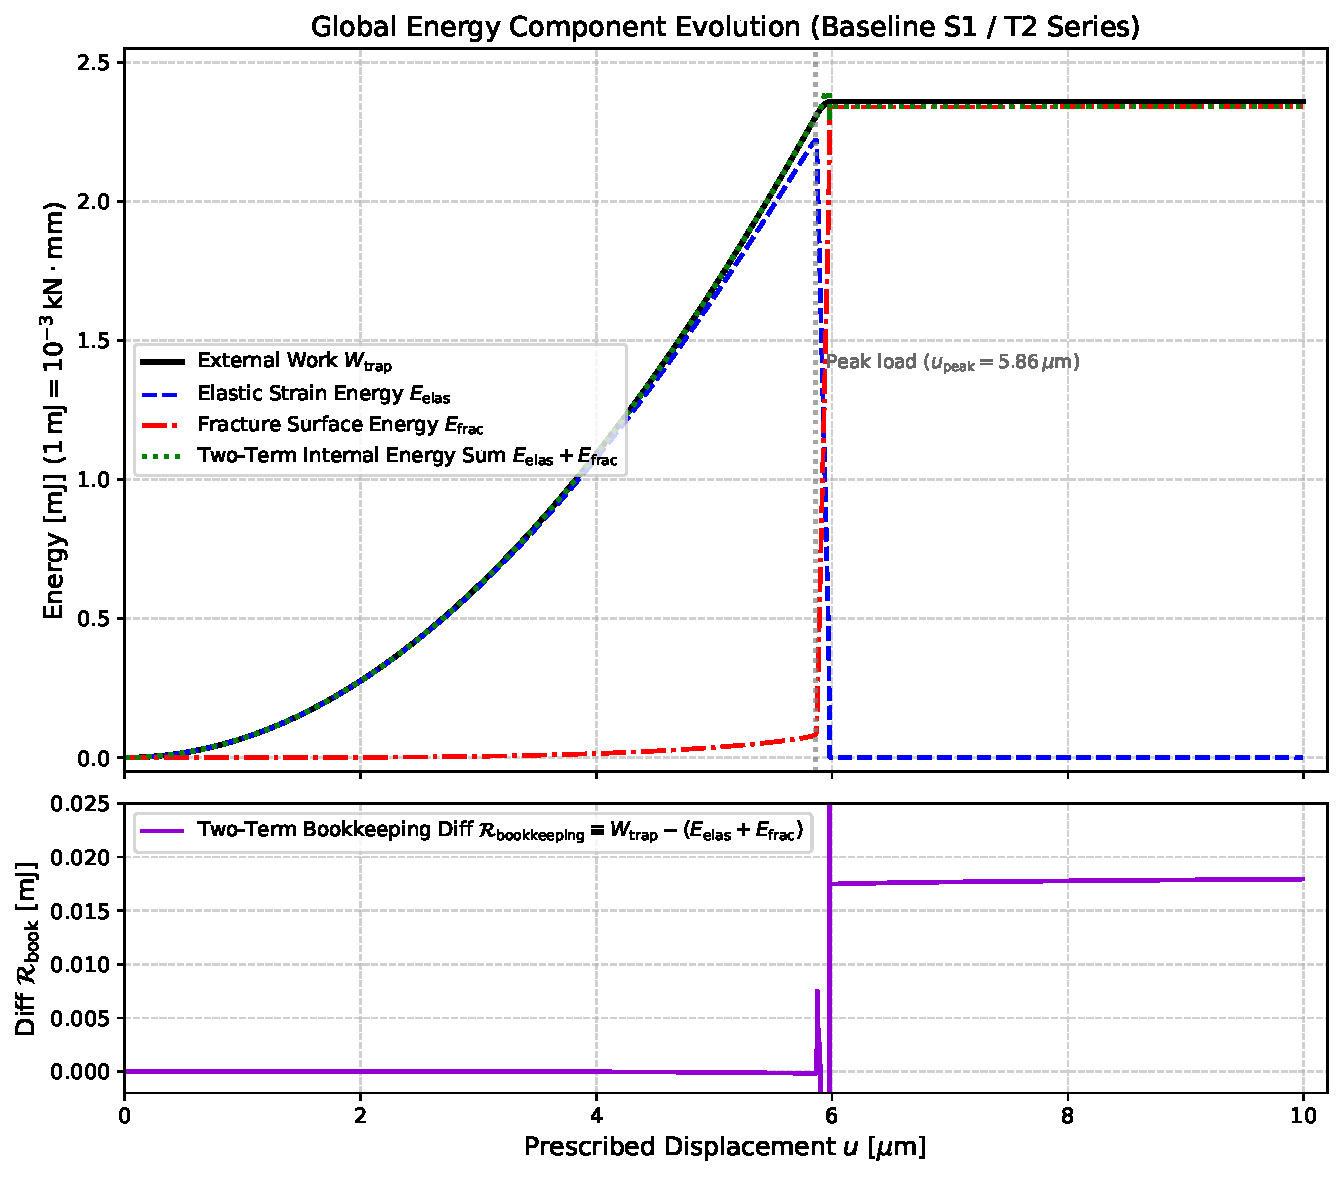
\includegraphics[width=0.82\textwidth]{fig_mode1_s1_energy_balance.pdf}
  \caption{Global energy component evolution for baseline $S_1$/$T_2$ ($15{,}192$ elements). The two-term bookkeeping difference remains within $\pm0.008\%$ over pre-peak deformation ($u \le 5.50\,\mu\mathrm{m}$). In the post-peak regime it reaches $+0.7607\%$ for $S_1$/$T_2$. This quantity is an observed endpoint bookkeeping difference: \textbf{\texttt{GLOBAL\_ENERGY\_IDENTITY --- NOT\_YET\_CLOSED}}.}
  \label{fig:energy_balance_pack}
  \figureconclusion{Before propagation, boundary work and $E_{\mathrm{elas}}+E_{\mathrm{frac}}$ track closely; during rapid fracture, elastic energy falls as fracture energy rises. The post-peak difference is an observed balance residual, not proof of global conservation: \texttt{GLOBAL\_ENERGY\_IDENTITY --- NOT\_YET\_CLOSED}.}
\end{figure}

\subsection{Temporal Discretization Scaling of Global Energy Components ($T_1$--$T_3$)}
Figure~\ref{fig:temporal_energy_pack} and Table~\ref{tab:energy_audit_pack} evaluate the temporal sensitivity of all energetic components across time increment scales ($T_1$: coarse $2\times$, $T_2$: nominal $1\times$, $T_3$: fine $0.5\times$):
\begin{itemize}
  \item Stored elastic strain energy $E_{\mathrm{elas}}(u)$ and fracture surface energy $E_{\mathrm{frac}}(u)$ exhibit excellent temporal agreement throughout deformation. During rapid crack propagation, $E_{\mathrm{elas}}$ decreases while $E_{\mathrm{frac}}$ increases.
  \item Pre-peak boundary work $W_{\mathrm{trap}}$ is temporally invariant ($|\Delta| < 0.001\%$). In the post-peak softening tail, finer time stepping slightly decreases external boundary work ($2.41011 \to 2.35933 \to 2.33189\,\mathrm{mJ}$, a $3.24\%$ reduction), reflecting sharper resolution of the steep load drop.
  \item Consequently, the terminal two-term bookkeeping difference shifts from $+0.378\%$ ($T_1$) to $+0.761\%$ ($T_2$) to $+3.541\%$ ($T_3$), establishing that post-peak bookkeeping values are \textbf{\texttt{TEMPORALLY SENSITIVE}}.
\end{itemize}

\begin{figure}[htbp]
  \centering
  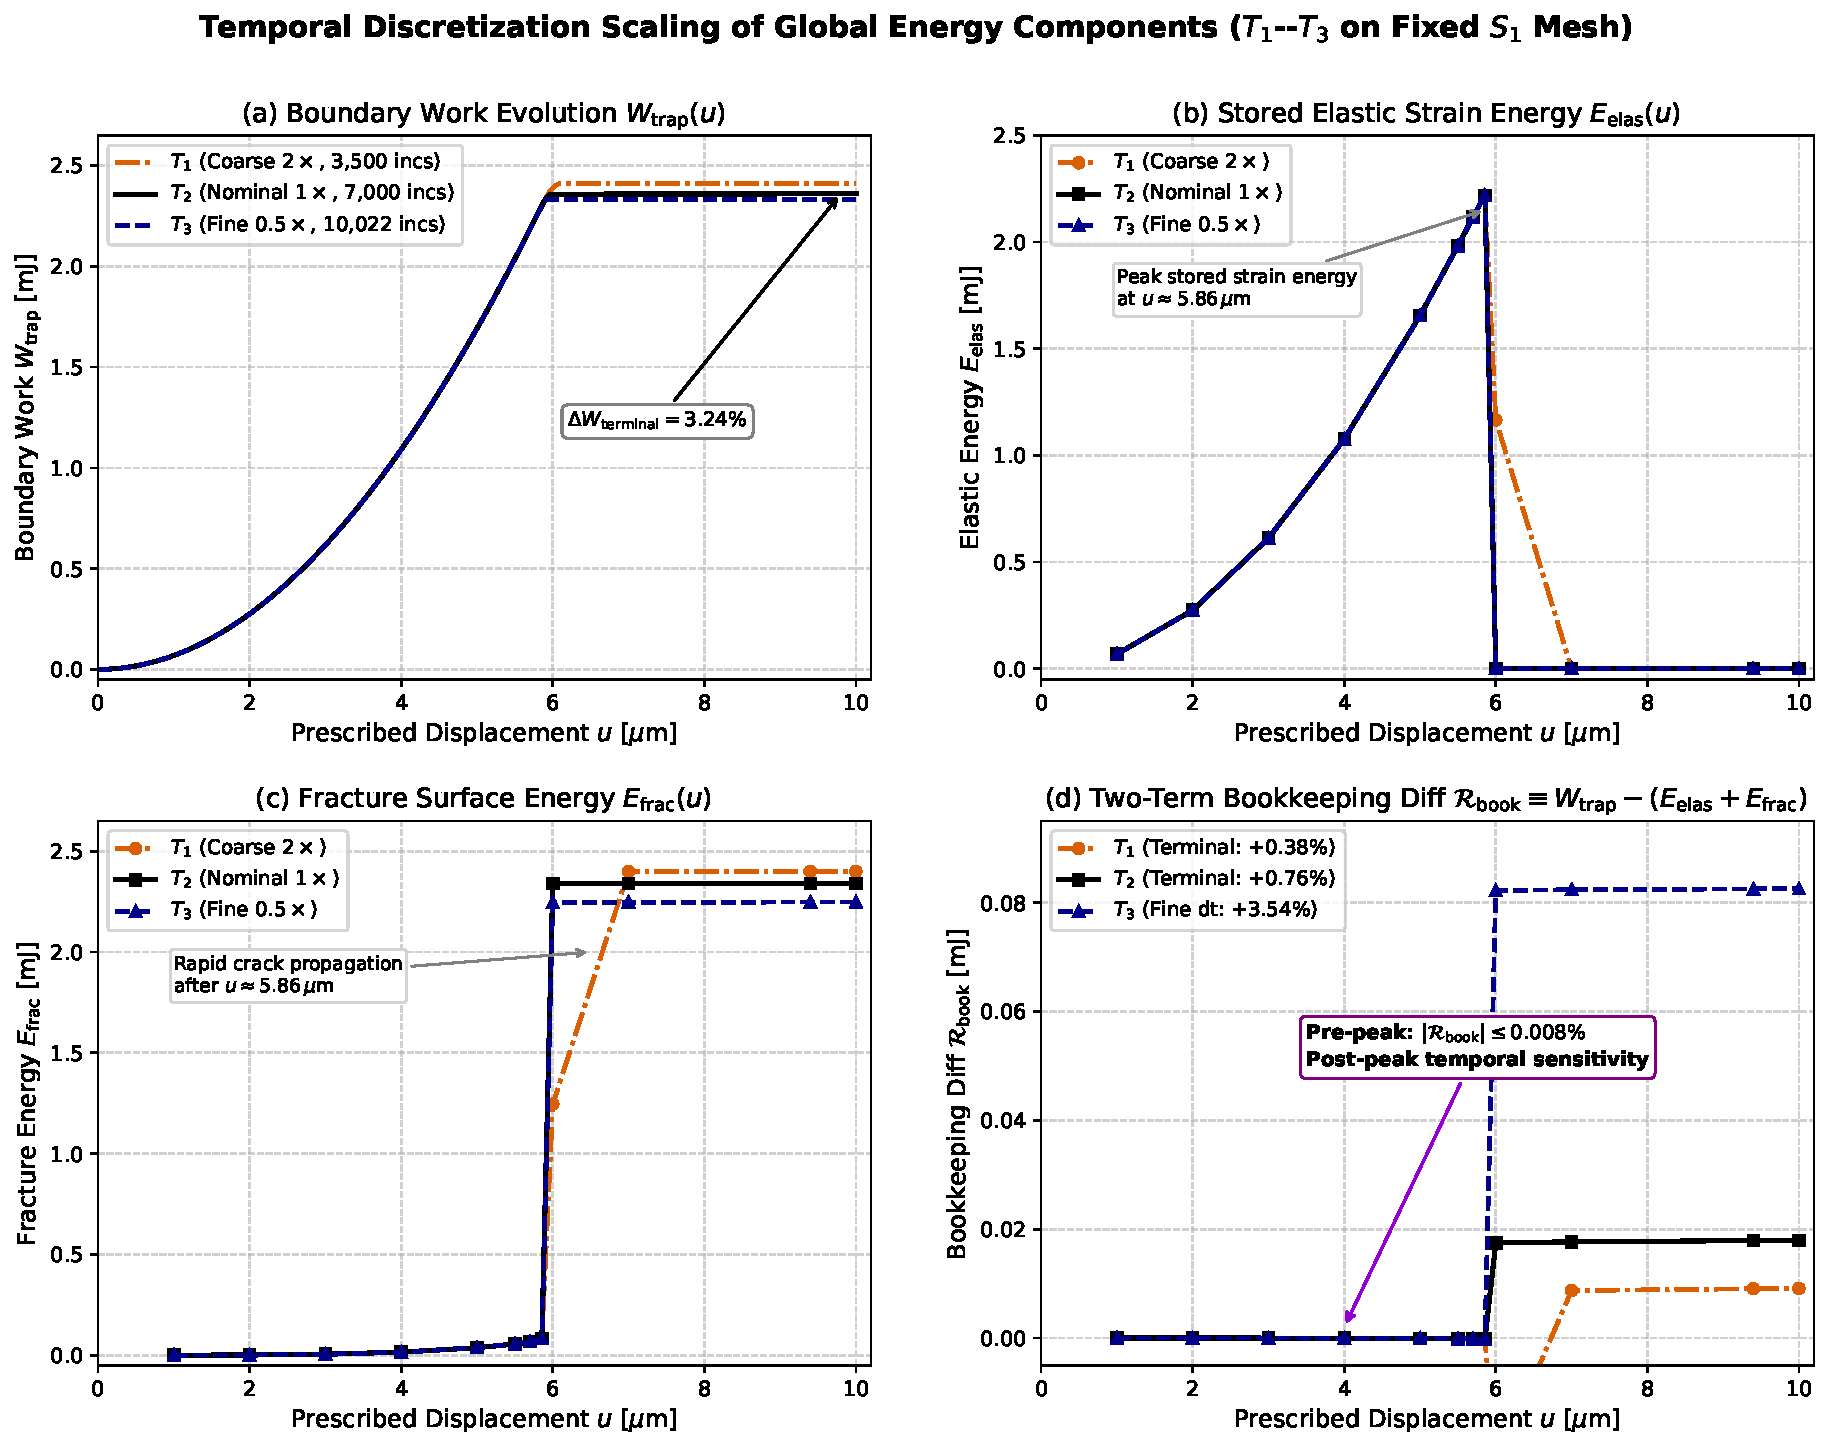
\includegraphics[width=0.92\textwidth]{fig_mode1_temporal_energy_comparison.pdf}
  \caption{Temporal discretization scaling of global energy components across schedules $T_1$ ($2\times$), $T_2$ ($1\times$), and $T_3$ ($0.5\times$, Job \texttt{1406317}) on fixed $S_1$ mesh: (a) boundary work $W_{\mathrm{trap}}(u)$; (b) stored elastic energy $E_{\mathrm{elas}}(u)$; (c) fracture surface energy $E_{\mathrm{frac}}(u)$; (d) two-term bookkeeping difference $\Delta_{\mathrm{book}}(u)$.}
  \label{fig:temporal_energy_pack}
  \figureconclusion{$E_{\mathrm{elas}}$ and $E_{\mathrm{frac}}$ remain similar across $T_1$--$T_3$, but terminal $W_{\mathrm{trap}}$ changes by $3.24\%$ and $\Delta_{\mathrm{book}}$ changes from $+0.378\%$ to $+3.541\%$. Mechanical peak convergence does not imply post-peak energetic convergence.}
\end{figure}

\begin{table}[htbp]
\centering
\caption{Global energy bookkeeping audit for completed uniform mesh cases ($u = 0.010\,\mathrm{mm}$).}
\label{tab:energy_audit_pack}
\small
\begin{tabularx}{\textwidth}{Yrrrr}
\toprule
Energetic Quantity & Case $T_1$ (Coarse $\Delta t$) & Case $T_2$ (Nominal $\Delta t$) & Case $T_3$ (Fine $\Delta t$) & Case $S_1$ (Baseline) \\
\midrule
Boundary Work $W_{\mathrm{trap}}$ [$\mathrm{mJ}$] & $2.41011$ & $2.35933$ & $2.33189$ & $2.35933$ \\
Elastic Energy $E_{\mathrm{elas}}$ [$\mathrm{mJ}$] & $0.00104$ & $0.00116$ & $0.00120$ & $0.00116$ \\
Fracture Energy $E_{\mathrm{frac}}$ [$\mathrm{mJ}$] & $2.39995$ & $2.34022$ & $2.24813$ & $2.34022$ \\
Bookkeeping Diff [$\mathrm{mJ}$] & $0.00912$ & $0.01795$ & $0.08256$ & $0.01795$ \\
Bookkeeping Diff [\%] & $+0.3783\%$ & $+0.7607\%$ & $+3.5407\%$ & $+0.7607\%$ \\
\midrule
Status & \texttt{TEMPORALLY SENSITIVE} & Baseline Anchor & \texttt{TEMPORALLY SENSITIVE} & Baseline Anchor \\
\bottomrule
\end{tabularx}
\end{table}

\subsection{Spatial Discretization Convergence of Global Energy Components ($S_1$--$S_4$)}
\label{subsec:spatial_energy_convergence}
The spatial convergence of UEL energetic quantities is rigorously evaluated across the four authoritative governed fixed meshes: $S_1$ ($h = 3.00\,\mu\mathrm{m}$, $15{,}192$ elements, Job \texttt{1406015}), $S_2$ ($h = 2.00\,\mu\mathrm{m}$, $32{,}130$ elements, Job \texttt{1406016}), $S_3$ ($h = 1.50\,\mu\mathrm{m}$, $41{,}912$ elements, Job \texttt{1406017}), and $S_4$ ($h = 1.25\,\mu\mathrm{m}$, $51{,}408$ elements, Job \texttt{1406018}).

Table~\ref{tab:spatial_energy_convergence} and Figure~\ref{fig:spatial_energy_convergence_pack} present the matched-displacement comparison at the three accepted physical checkpoints:
\begin{enumerate}[leftmargin=*]
  \item \textbf{Pre-Peak Elastic and Damage Initiation ($u = 5.50\,\mu\mathrm{m}$):}
    \begin{itemize}
      \item External boundary work $W_{\mathrm{trap}}$ is tightly invariant across meshes ($2.03739 \to 2.03528\,\mathrm{mJ}$, $-0.10\%$), classified \textbf{\texttt{STABLE\_OVER\_TESTED\_RANGE}}.
      \item Stored elastic strain energy $E_{\mathrm{elas}}$ constitutes over $97.1\%$ of total input work and varies by $-0.23\%$ ($1.98181 \to 1.97717\,\mathrm{mJ}$), classified \textbf{\texttt{STABLE\_OVER\_TESTED\_RANGE}}.
      \item Regularized fracture surface energy $E_{\mathrm{frac}}$ accounts for the remaining $2.9\%$ of input work, increasing smoothly from $0.05572\,\mathrm{mJ}$ ($S_1$) to $0.05815\,\mathrm{mJ}$ ($S_4$, $+4.36\%$), classified \textbf{\texttt{MESH-SENSITIVE}}.
      \item The two-term bookkeeping difference $\Delta_{\mathrm{book}}$ is strictly negligible in this pre-peak regime ($-0.00014\,\mathrm{mJ}$ to $-0.00004\,\mathrm{mJ}$, $< 0.007\%$ of $W_{\mathrm{trap}}$).
    \end{itemize}
  \item \textbf{Near-Peak / Early Softening Transition ($u = 5.85\,\mu\mathrm{m}$):}
    Reflects the mesh-induced peak displacement shift ($u_{\mathrm{peak}} = 5.857\,\mu\mathrm{m}$ for $S_1$ vs $5.586\,\mu\mathrm{m}$ for $S_4$). Baseline $S_1$ resides directly at its load peak ($F = 0.75756\,\mathrm{kN}$), whereas refined meshes $S_2$--$S_4$ have already undergone rapid crack extension ($F < 0.0003\,\mathrm{kN}$, $E_{\mathrm{frac}} \approx 2.33 - 2.38\,\mathrm{mJ}$).
  \item \textbf{Post-Peak Fully Fractured State ($u = 6.20\,\mu\mathrm{m}$):}
    \begin{itemize}
      \item All four models have completely severed the ligament ($d_{\max} \ge 1.0004$, residual load $F < 0.0006\,\mathrm{kN}$, $E_{\mathrm{elas}} < 0.0016\,\mathrm{mJ} \approx 0$).
      \item Regularized fracture surface energy evaluated across the meshes gives $E_{\mathrm{frac}} = 2.33886\,\mathrm{mJ}$ ($S_1$), $2.33022\,\mathrm{mJ}$ ($S_2$, $-0.37\%$), $2.35701\,\mathrm{mJ}$ ($S_3$, $+0.78\%$), and $2.37531\,\mathrm{mJ}$ ($S_4$, $+1.56\%$). The full min--max spread across $S_1$--$S_4$ is \textbf{$1.94\%$}, classified as \textbf{\texttt{STABLE\_OVER\_TESTED\_RANGE}}.
      \item External boundary work $W_{\mathrm{trap}}$ decreases from $2.35801\,\mathrm{mJ}$ ($S_1$) to $2.17004\,\mathrm{mJ}$ ($S_4$, $-7.97\%$), classified \textbf{\texttt{MESH-SENSITIVE}}.
      \item The resulting post-peak two-term difference $\Delta_{\mathrm{book}}$ ranges from $+0.01754\,\mathrm{mJ}$ ($+0.74\%$ for $S_1$) to $-0.20585\,\mathrm{mJ}$ ($-9.49\%$ for $S_4$), strictly designated as an observed balance residual under \textbf{\texttt{GLOBAL\_ENERGY\_IDENTITY --- NOT\_YET\_CLOSED}}.
    \end{itemize}
\end{enumerate}

\begin{figure}[htbp]
  \centering
  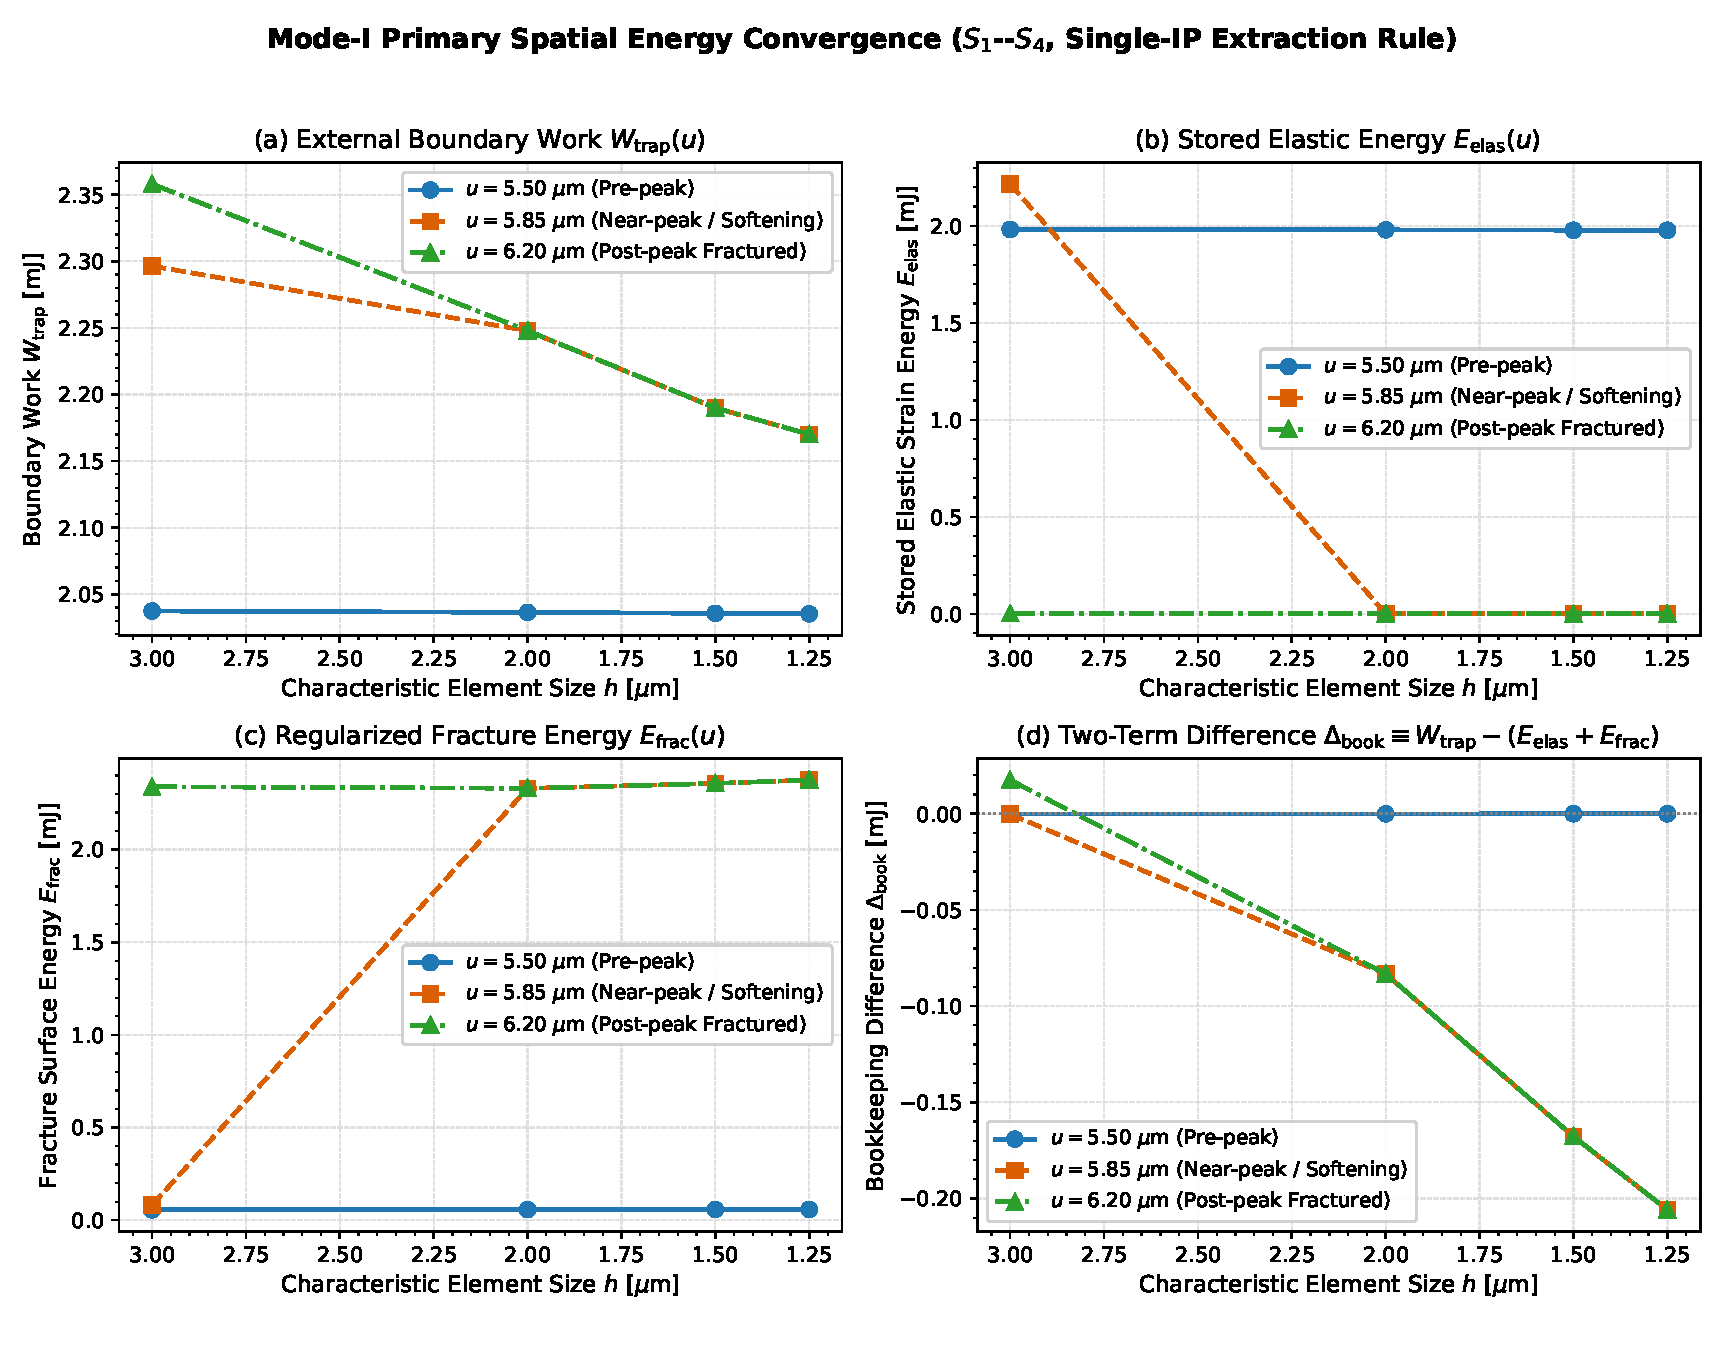
\includegraphics[width=0.92\textwidth]{fig_mode1_spatial_energy_convergence.pdf}
  \caption{Spatial discretization convergence of global energy components across meshes $S_1$--$S_4$ at matched displacements $u = 5.50, 5.85, 6.20\,\mu\mathrm{m}$: (a) boundary work $W_{\mathrm{trap}}$; (b) stored elastic strain energy $E_{\mathrm{elas}}$; (c) regularized fracture surface energy $E_{\mathrm{frac}}$; (d) two-term bookkeeping difference $\Delta_{\mathrm{book}}$. \textbf{\texttt{GLOBAL\_ENERGY\_IDENTITY --- NOT\_YET\_CLOSED}}.}
  \label{fig:spatial_energy_convergence_pack}
  \figureconclusion{At $u=5.50\,\mu\mathrm{m}$, boundary work and elastic energy are spatially stable. After fracture, $E_{\mathrm{frac}}$ is comparatively stable ($S_1\rightarrow S_4$: $+1.56\%$; full spread: $1.94\%$), while $W_{\mathrm{trap}}$ and $\Delta_{\mathrm{book}}$ remain mesh-sensitive. A closed global energy identity has not been demonstrated.}
\end{figure}

\begin{table}[htbp]
\centering
\caption{Spatial energy convergence audit across fixed meshes $S_1$--$S_4$ at matched displacements.}
\label{tab:spatial_energy_convergence}
\fontsize{7.0}{8.5}\selectfont
\setlength{\tabcolsep}{2.5pt}
\begin{tabular*}{\textwidth}{@{\extracolsep{\fill}}lrrrrrrrl@{}}
\toprule
\textbf{Model ($h$)} & \textbf{Elements} & \textbf{$F(u)$ [kN]} & \textbf{$W_{\mathrm{trap}}$ [mJ]} & \textbf{$E_{\mathrm{elas}}$ [mJ]} & \textbf{$E_{\mathrm{frac}}$ [mJ]} & \textbf{$E_{\mathrm{tot}}$ [mJ]} & \textbf{$\Delta_{\mathrm{book}}$ [mJ]} & \textbf{Classification} \\
\midrule
\multicolumn{9}{l}{\textbf{State 1: Pre-peak initiation ($u = 5.50\,\mu\mathrm{m}$)}} \\
$S_1$ ($3.00\,\mu\mathrm{m}$) & $15{,}192$ & $0.72066$ & $2.03739$ & $1.98181$ & $0.05572$ & $2.03753$ & $-0.00014$ & Baseline Qualified \\
$S_2$ ($2.00\,\mu\mathrm{m}$) & $32{,}130$ & $0.71984$ & $2.03635$ & $1.97957$ & $0.05686$ & $2.03643$ & $-0.00008$ & \texttt{STABLE} ($-0.05\%$) \\
$S_3$ ($1.50\,\mu\mathrm{m}$) & $41{,}912$ & $0.71925$ & $2.03565$ & $1.97795$ & $0.05775$ & $2.03570$ & $-0.00005$ & \texttt{STABLE} ($-0.09\%$) \\
$S_4$ ($1.25\,\mu\mathrm{m}$) & $51{,}408$ & $0.71897$ & $2.03528$ & $1.97717$ & $0.05815$ & $2.03532$ & $-0.00004$ & \texttt{STABLE} ($-0.10\%$) \\
\midrule
\multicolumn{9}{l}{\textbf{State 2: Near-peak / softening transition ($u = 5.85\,\mu\mathrm{m}$)}} \\
$S_1$ ($3.00\,\mu\mathrm{m}$) & $15{,}192$ & $0.75756$ & $2.29636$ & $2.21586$ & $0.08068$ & $2.29654$ & $-0.00018$ & Peak State ($u_{\mathrm{peak}}=5.857\,\mu\mathrm{m}$) \\
$S_2$ ($2.00\,\mu\mathrm{m}$) & $32{,}130$ & $0.00031$ & $2.24774$ & $0.00090$ & $2.33015$ & $2.33105$ & $-0.08331$ & Post-softening ($d_{\max}=1.0006$) \\
$S_3$ ($1.50\,\mu\mathrm{m}$) & $41{,}912$ & $0.00023$ & $2.18985$ & $0.00067$ & $2.35696$ & $2.35763$ & $-0.16778$ & Post-softening ($d_{\max}=1.0007$) \\
$S_4$ ($1.25\,\mu\mathrm{m}$) & $51{,}408$ & $0.00020$ & $2.16997$ & $0.00057$ & $2.37528$ & $2.37585$ & $-0.20588$ & Post-softening ($d_{\max}=1.0006$) \\
\midrule
\multicolumn{9}{l}{\textbf{State 3: Post-peak fully fractured state ($u = 6.20\,\mu\mathrm{m}$)}} \\
$S_1$ ($3.00\,\mu\mathrm{m}$) & $15{,}192$ & $0.00052$ & $2.35801$ & $0.00161$ & $2.33886$ & $2.34047$ & $+0.01754$ & Broken Baseline ($d_{\max}=1.0004$) \\
$S_2$ ($2.00\,\mu\mathrm{m}$) & $32{,}130$ & $0.00028$ & $2.24785$ & $0.00087$ & $2.33022$ & $2.33110$ & $-0.08325$ & $E_{\mathrm{frac}}$ \texttt{STABLE} ($-0.37\%$) \\
$S_3$ ($1.50\,\mu\mathrm{m}$) & $41{,}912$ & $0.00021$ & $2.18993$ & $0.00066$ & $2.35701$ & $2.35767$ & $-0.16774$ & $E_{\mathrm{frac}}$ \texttt{STABLE} ($+0.78\%$) \\
$S_4$ ($1.25\,\mu\mathrm{m}$) & $51{,}408$ & $0.00018$ & $2.17004$ & $0.00057$ & $2.37531$ & $2.37589$ & $-0.20585$ & $E_{\mathrm{frac}}$ \texttt{STABLE} ($+1.56\%$) \\
\bottomrule
\end{tabular*}
\end{table}

\subsection{Itemized Energetic Qualification Status Summary}
Table~\ref{tab:energy_qualification_status} provides the definitive itemized status of all energetic expressions, separating verified source terms, derived relations, and unclosed physical questions.

\begin{table}[htbp]
\centering
\caption{Definitive energetic quantity classification and qualification status.}
\label{tab:energy_qualification_status}
\fontsize{7.5}{9.0}\selectfont
\begin{tabularx}{\textwidth}{lXll}
\toprule
\textbf{Quantity} & \textbf{Mathematical Definition / Extraction} & \textbf{Units} & \textbf{Status} \\
\midrule
$K_0$ & $dF/du|_{\text{elastic}}$ (RP 999999 $RF_2$) & $\mathrm{kN/mm}$ & \textbf{\texttt{NUMERICALLY\_VERIFIED}} \\
$F_{\max}, u_{\mathrm{peak}}$ & Peak reaction force and displacement & $\mathrm{kN}, \mathrm{mm}$ & \textbf{\texttt{NUMERICALLY\_VERIFIED}} \\
$W_{\mathrm{trap}}$ & $\sum \frac{1}{2}(F_n+F_{n-1})(u_n-u_{n-1})$ & $\mathrm{kN\cdot mm} \equiv \mathrm{J}$ & \textbf{\texttt{DERIVED\_AND\_CHECKED}} \\
$\psi_e$ & $\frac{1}{2}g(d)\boldsymbol{\varepsilon}:\mathbb{C}_0:\boldsymbol{\varepsilon}$ & $\mathrm{kN/mm^2} = \mathrm{J/mm^3}$ & \textbf{\texttt{VERIFIED\_FROM\_SOURCE}} \\
$E_{\mathrm{elas}}$ & $\int_{\Omega} \psi_e\,\mathrm{d}\Omega \to \texttt{ENERGY(2)} \to \texttt{ALLSE}$ & $\mathrm{kN\cdot mm} \equiv \mathrm{J}$ & \textbf{\texttt{VERIFIED\_FROM\_SOURCE}} \\
$\psi_f$ & $G_c [ d^2/(2l_0) + (l_0/2)|\nabla d|^2 ]$ & $\mathrm{kN/mm^2} = \mathrm{J/mm^3}$ & \textbf{\texttt{VERIFIED\_FROM\_SOURCE}} \\
$E_{\mathrm{frac}}$ & $\int_{\Omega} \psi_f\,\mathrm{d}\Omega \to \mathrm{STATEV}(17), \texttt{CSV}$ & $\mathrm{kN\cdot mm} \equiv \mathrm{J}$ & \textbf{\texttt{VERIFIED\_FROM\_SOURCE}} \\
Pre-peak $\Delta_{\mathrm{book}}$ & $|\Delta_{\mathrm{book}}| / W_{\mathrm{trap}} < 0.007\%$ & Dimensionless & \textbf{\texttt{NUMERICALLY\_VERIFIED}} \\
Post-peak $\Delta_{\mathrm{book}}$ & $W_{\mathrm{trap}} - (E_{\mathrm{elas}}+E_{\mathrm{frac}})$ residual ($-9.49\%$) & $\mathrm{kN\cdot mm} \equiv \mathrm{J}$ & \textbf{\texttt{NUMERICALLY\_VERIFIED (OBSERVED)}} \\
$\mathcal{D}_{\mathrm{frac}}$ & $\int_0^t \int_{\Omega} 2(1-d)\mathcal{H}\dot{d}\,\mathrm{d}\Omega\,\mathrm{d}\tau$ & $\mathrm{kN\cdot mm} \equiv \mathrm{J}$ & \textbf{\texttt{NOT\_YET\_QUALIFIED}} \\
$\mathcal{D}_{\mathrm{frac}} = \dot{E}_{\mathrm{frac}}$ & Rate equality under active damage & $\mathrm{W}$ & \textbf{\texttt{NOT\_YET\_QUALIFIED}} \\
\bottomrule
\end{tabularx}
\end{table}

\clearpage

\section{Epistemological Audit, Claim Ledger, and Supervisory Decisions}
\label{sec:epistemological_audit_and_decisions}

\subsection{Compact Supervisor-Facing Claim Ledger}
Table~\ref{tab:claim_ledger_pack} classifies the standing of all findings into three mutually exclusive categories: THEORY, VERIFIED NUMERICAL EVIDENCE, and UNRESOLVED.

\begin{table}[htbp]
\centering
\caption{Compact Mode-I Claim Ledger across Core Physical and Energetic Metrics.}
\label{tab:claim_ledger_pack}
\scriptsize
\setlength{\tabcolsep}{3pt}
\begin{tabularx}{\textwidth}{p{2.2cm}p{3.8cm}p{4.2cm}X}
\toprule
Metric / Aspect & \textbf{THEORY} (Continuum / Formulation) & \textbf{VERIFIED EVIDENCE} (Audited Artifacts) & \textbf{UNRESOLVED} (Boundaries / Open Scope) \\
\midrule
1. Initial Stiffness $K_0$ & Continuum linear elasticity ($\boldsymbol{\sigma} = \mathbb{C}_0 : \boldsymbol{\varepsilon}$) provides reference stiffness. & $K_0 = 137.84$--$137.95\,\mathrm{kN/mm}$ ($\Delta < 0.08\%$ spatial across $S_1$--$S_4$, $\Delta < 0.001\%$ temporal across $T_1$--$T_3$). Baseline $S_1$: $137.9455\,\mathrm{kN/mm}$. & None for standard Mode-I; \textbf{\texttt{CONVERGED / STABLE}}. \\
\addlinespace
2. Spatial Peak Force $F_{\max}$ & Degradation $g(d) = (1-d)^2 + k_{\mathrm{res}}$ couples strain energy to damage evolution. & Monotonic reduction: $F_{\max} = 0.7578\,\mathrm{kN}$ ($S_1$) $\to 0.7312\,\mathrm{kN}$ ($S_4$) $\to 0.7255\,\mathrm{kN}$ (historical fine mesh), $4.26\%$ drop across $h/l_0 \in [0.133, 0.400]$. & Asymptotic spatial convergence is not established within the tested mesh range; \textbf{\texttt{MESH-SENSITIVE}}. \\
\addlinespace
3. Temporal Peak Force $F_{\max}$ & Temporal invariance of limit load under $\Delta t$ scaling. & Invariant: $F_{\max} = 0.75815\,\mathrm{kN}$ ($T_1$) $\to 0.75763\,\mathrm{kN}$ ($T_3$), spread $\Delta < 0.069\%$. & None across tested time-step range; \textbf{\texttt{CONVERGED / STABLE}}. \\
\addlinespace
4. Pre-Peak Work $W_{\mathrm{trap}}$ & Trapezoidal boundary-work estimate $W_{\mathrm{trap},n} = \sum_{i=1}^{n} \frac{F_i+F_{i-1}}{2}(u_i-u_{i-1})$. & $W_{\mathrm{trap}} \in [2.035, 2.038]\,\mathrm{mJ}$ at $u = 5.50\,\mu\mathrm{m}$ across tested cases ($\Delta < 0.15\%$). & Stable over tested pre-peak range; \textbf{\texttt{CONVERGED / STABLE}}. \\
\addlinespace
5. Terminal Work $W_{\mathrm{trap}}$ & Endpoint integral along displacement path. & Full runs: $W_{\mathrm{trap}} = 2.4101\,\mathrm{mJ}$ ($T_1$) $\to 2.3319\,\mathrm{mJ}$ ($T_3$) ($3.24\%$ variation); cutback runs truncated at $u=6.8$--$9.6\,\mu\mathrm{m}$. & Cross-mesh terminal comparison at unequal cutback endpoints is not qualified; \textbf{\texttt{TEMPORALLY SENSITIVE}}. \\
\addlinespace
6. Length-Scale ($l_0$) Sensitivity & Characteristic width of regularized damage band. & 3-point fixed-$S_3$ study: $l_0 \in \{7.5, 11.25, 15.0\}\,\mu\mathrm{m}$ yields $K_0$ spread $0.13\%$ (\textbf{\texttt{STABLE}}), $F_{\max}$ drop $5.83\%$ ($0.732 \to 0.690\,\mathrm{kN}$) and $u_{\mathrm{peak}}$ shift ($5.633 \to 5.579\,\mu\mathrm{m}$). & Terminal energy across unequal endpoints: \textbf{\texttt{NOT\_YET\_QUALIFIED\_UNEQUAL\_ENDPOINTS}}. \\
\addlinespace
7. UEL Energy Terms & Implemented integrals of $E_{\mathrm{elas}}$ and $E_{\mathrm{frac}}$ in \nolinkurl{f42_mixed_uel.for}. & Unit-105 CSV and ODB IP1: $E_{\mathrm{elas}} = 1.1608\times 10^{-3}\,\mathrm{mJ}$, $E_{\mathrm{frac}} = 2.34021\,\mathrm{mJ}$; matched-displacement spatial energy convergence is quantified for $S_1$--$S_4$. & Terminal cross-mesh energy comparison at unequal cutback endpoints is not qualified. \\
\addlinespace
8. Bookkeeping Difference & Algebraic difference $W_{\mathrm{trap}} - (E_{\mathrm{elas}} + E_{\mathrm{frac}})$. & Baseline $S_1$: $+0.7607\%$ ($+1.795\times 10^{-2}\,\mathrm{mJ}$); $T_1 \to T_3$: $+0.378\% \to +3.541\%$. & Exact decomposition requires within-increment path; \textbf{\texttt{TEMPORALLY SENSITIVE}}. \\
\addlinespace
9. Global Energy Identity & Staggered solution scheme lacks joint discrete scalar potential. & Non-commutativity $\partial^2 \Pi / \partial \mathbf{u} \partial d \ne \partial^2 \Pi / \partial d \partial \mathbf{u}$; ODB does not record within-increment paths. & \textbf{\texttt{GLOBAL\_ENERGY\_IDENTITY --- NOT\_YET\_CLOSED}}. \\
\addlinespace
10. Damage-Weighted Crack-Centroid Trajectory & Symmetric Mode-I crack extension along centerline $y = 0.500\,\mathrm{mm}$. & Centroid offset $|y_c - 0.5\,\mathrm{mm}| \le 3.10\,\mu\mathrm{m}$ across all meshes; bounded within single element dimension. & Pure Mode-I symmetry preserved; \textbf{\texttt{CONVERGED / STABLE}}. \\
\bottomrule
\end{tabularx}
\end{table}

\subsection{Decisions and Direction Requested for 08 October Meeting}
\begin{enumerate}
  \item \textbf{Mode-I Foundations Approval:} Review and formal acceptance of the updated Mode-I thesis chapters (Chapters 1--3, 7--8) incorporating all verified mechanical, adaptive, and energetic findings.
  \item \textbf{Supervisor Decision on Gate 6B Closure:} Supervisory ruling on accepting the endpoint energetic qualification and acknowledging the formal epistemic boundary \textbf{\texttt{GLOBAL\_ENERGY\_IDENTITY --- NOT\_YET\_CLOSED}} as the closed state of Gate~6B.
  \item \textbf{Authorization to Proceed to Gate 6C:} Transition to Gate~6C (State Transfer Energy Preservation) upon formal closure of Gate~6B.
  \item \textbf{Maintenance of Scope Holds:} Confirmation that Mode-II, multi-crack configurations, and Gate~7 visualization remain paused until Gate~6C state transfer is completed.
\end{enumerate}

\clearpage

\section{Job Ledger, Artifact Provenance, and References}
\label{sec:provenance_and_references}

\subsection{Authoritative Job Ledger}
Table~\ref{tab:job_ledger_pack} lists the key Abaqus simulations constituting the Mode-I evidence base, executed on the TU Bergakademie Freiberg HPC cluster (\texttt{mmaster02}, queue \texttt{normal\_imfdfkmq}).

\begin{table}[htbp]
\centering
\caption{Authoritative HPC Job Ledger for the Mode-I Benchmark Series.}
\label{tab:job_ledger_pack}
\scriptsize
\setlength{\tabcolsep}{3pt}
\begin{tabularx}{\textwidth}{llYlrl}
\toprule
Job ID & Model Name & Description & Input Deck Hash & Elements & Exit Status \\
\midrule
\texttt{1406015.mmaster02} & \texttt{PK\_M1\_S1\_H0030} & Canonical spatial baseline $S_1$ ($h=3.0\,\mu\mathrm{m}$) & \texttt{bc000e0c579...} & $15{,}192$ & \texttt{Exit\_status=0} \\
\texttt{1398090.mmaster02} & \texttt{PK\_M1\_FIX\_REF} & Historical reference anchor & \texttt{a845ef1a37c...} & $15{,}192$ & \texttt{Exit\_status=0} \\
\texttt{1404933.mmaster02} & \texttt{PK\_M1\_NOM1\_1404933} & Corrected 71k full fracture & \texttt{72674e2ba05...} & $71{,}320$ & \texttt{Exit\_status=0} \\
\texttt{1405044.mmaster02} & \texttt{PK\_M1\_FROZEN\_71K} & Frozen elastic requalification & \texttt{3bbdfb9a528...} & $71{,}320$ & \texttt{Exit\_status=0} \\
\texttt{1406016.mmaster02} & \texttt{PK\_M1\_S2\_H0020} & Spatial fine $S_2$ ($h=2.0\,\mu\mathrm{m}$) & \texttt{34ec7f0b5d0...} & $32{,}130$ & \texttt{Exit\_status=0} (Cutback) \\
\texttt{1406017.mmaster02} & \texttt{PK\_M1\_S3\_H0015} & Spatial fine $S_3$ ($h=1.5\,\mu\mathrm{m}, l_0=7.5\,\mu\mathrm{m}$) & \texttt{eb009f188a2...} & $41{,}912$ & \texttt{Exit\_status=0} (Cutback) \\
\texttt{1406018.mmaster02} & \texttt{PK\_M1\_S4\_H00125} & Spatial fine $S_4$ ($h=1.25\,\mu\mathrm{m}$) & \texttt{cc88dfd1b08...} & $51{,}408$ & \texttt{Exit\_status=0} (Cutback) \\
\texttt{1406019.mmaster02} & \texttt{PK\_M1\_S5\_H00100} & Historical fine ($h=1.0\,\mu\mathrm{m}$; legacy model name; not governed $S_5$) & \texttt{634b3d758f8...} & $69{,}384$ & \texttt{Exit\_status=0} (Cutback) \\
\texttt{1406020.mmaster02} & \texttt{PK\_M1\_T1\_DT2X} & Temporal coarse $T_1$ ($2.0\times\Delta t$) & \texttt{ad9dfa6d899...} & $15{,}192$ & \texttt{Exit\_status=0} \\
\texttt{1406021.mmaster02} & \texttt{PK\_M1\_T2\_DT1X} & Temporal nominal $T_2$ ($1.0\times\Delta t$) & \texttt{fa88301c272...} & $15{,}192$ & \texttt{Exit\_status=0} \\
\texttt{1406317.mmaster02} & \texttt{PK\_M1\_T3\_DT05X\_R2} & Temporal fine $T_3$ ($0.5\times\Delta t$) & \texttt{92562479633...} & $15{,}192$ & \texttt{Exit\_status=0} (Full) \\
\texttt{1406278.mmaster02} & \texttt{PK\_M1\_A2\_2PCT} & Adaptive $A_2$ (2\% errorTarget) & \texttt{d4ec8aa9ebf...} & $15{,}396$ & \texttt{Exit\_status=0} \\
\texttt{1406273.mmaster02} & \texttt{PK\_M1\_A3\_3PCT} & Adaptive $A_3$ (3\% errorTarget) & \texttt{bb185fca481...} & $7{,}633$ & \texttt{Exit\_status=0} \\
\texttt{1406311.mmaster02} & \texttt{PK\_M1\_A3\_FINE\_DT} & Adaptive $A_3$ fine $\Delta t$ ($0.5\times$) & \texttt{8c14cf29b4e...} & $7{,}633$ & \texttt{Exit\_status=0} \\
\texttt{1406279.mmaster02} & \texttt{PK\_M1\_A4\_5PCT} & Adaptive $A_4$ (5\% errorTarget) & \texttt{82bcf2ff1c5...} & $4{,}194$ & \texttt{Exit\_status=0} \\
\texttt{1406839.mmaster02} & \texttt{PK\_M1\_S1\_DIAG\_R2} & Historical diagnostic energy-output run; non-authoritative for canonical $S_1$ provenance & \texttt{fa88301c272...} & $15{,}192$ & \texttt{Exit\_status=0} \\
\texttt{1406895.mmaster02} & \texttt{PK\_M1\_S3\_L01125} & $l_0 = 11.25\,\mu\mathrm{m}$ on fixed $S_3$ mesh & \texttt{77df64d10d0...} & $41{,}912$ & \texttt{Exit\_status=0} (Full) \\
\texttt{1406896.mmaster02} & \texttt{PK\_M1\_S3\_L01500} & $l_0 = 15.00\,\mu\mathrm{m}$ on fixed $S_3$ mesh & \texttt{ff13ba60800...} & $41{,}912$ & \texttt{Exit\_status=0} (Full) \\
\bottomrule
\end{tabularx}
\end{table}

\subsection{Subroutine Integrity}
The authoritative user subroutine \nolinkurl{f42_mixed_uel.for} governing all production calculations has the immutable cryptographic hash:
\begin{center}
  \texttt{SHA256: 5cd0d2c015c9ead91c99d7a744156cc86f5b5ea26473bbed7d6e5515fe30fa46}
\end{center}

\bibliographystyle{abbrvnat}
\bibliography{literature}


\end{document}
